% GUIDA VELOCE:
% --------------------------------------------------------------------
% X INIZIA UN UNOVO CAPITOLO:
% \chapter{??? NOME CAPITOLO}}
% \section{ ?? }
% \subsection{ ?? }
%
% --------------------------------------------------------------------
% PAROLA CONTENUTA NEL GLOSSARIO:
% scrivere la parola seguita da $^g$
% esempio: User$^g$
%
% --------------------------------------------------------------------
% PER ANDARE A CAPO SENZA RIENTRO INSERIRE:
% \\
%
% --------------------------------------------------------------------

% GRASSETO:
% \textbf{parola}
%
% --------------------------------------------------------------------
% CORSIVO:
% \emph{parola}
% --------------------------------------------------------------------
% PER SCRIVERE IN ROSSO:
% \red{parola}
%
% --------------------------------------------------------------------
% PER SCRIVERE TRA VIRGOLETTE
% ''parola''
%
% --------------------------------------------------------------------
% PER EVITARE IL RIENTRO AUTOMATICO DI UN CAPOVERSO:
% \noindent testo....
%
% --------------------------------------------------------------------

% PER SCRIVERE CARATTERI PARTICOLARI COME: { } _ ecc.. SCRIVERLI PRECEDUTI DA \
% ES: \{ \_
%
% --------------------------------------------------------------------
% X INSERIRE UN LINK:
% \url{http://www.math.unipd.it/~tullio/IS-1/2011/Progetto/C3.pdf}
%
% --------------------------------------------------------------------
% PER COMMENTARE INTERE PARTI:
% \comment{ comment }
%
% --------------------------------------------------------------------
% PER SCRIVERE NOTE DURANTE IL TESTO:
% parola \footnote{ note riguardanti la parola }
%
% --------------------------------------------------------------------
% PER SCRIVERE CODICE SORGENTE:
%
% \lstset{language=c++,
% stringstyle=\color{blue}\textrm,
% commentstyle=\rmfamily, numbers= none}

% \begin{lstlisting}
% CODICE
% \end{lstlisting}
%
% --------------------------------------------------------------------
% !!!!!!!! PER COSE + COMPLESSE VEDI: !!!!!!!!!!!!!!!!!!!!!!!
% !!!!!!!! PMAC/latex/GUIDA LATEX!!!.tex !!!!!!!!!!!!!!!!!!!!!!!

% per tutto il resto chiedi a lory prima di fare/scrivere cazzate !!!!!!!!!!



\documentclass[10pt,a4paper]{book}

\usepackage[italian]{babel}
\usepackage[T1]{fontenc}
\usepackage[utf8x]{inputenc} % uso utf8x xk x linux, mentre latin1 è per windows
\usepackage{lmodern} %insieme di font molto completo consigliato da LatexFacile pg13 in basso
\usepackage{microtype} %migliora riempimento delle righe. vedi LatexImpaziente pg41
%attiva il rientro di ogni prima riga di ogni sezione: capitolo,paragrafo ecc. vd LatexImpaziente pg41
\usepackage{indentfirst}
\usepackage{graphicx} % per inseire immagini
\usepackage[usenames,dvipsnames]{color}
\usepackage{lastpage} %serve per poter scrivere page 1 of N
% setta i bordi della pagina: dx e sx 3.2cm di rientro + nel lato di rilagatura rientra di altri 0mm
\usepackage[a4paper,top=3cm,bottom=3cm,left=3.2cm,right=3.2cm, bindingoffset=0mm]{geometry}
\usepackage{listings} % per inserire codice sorgente
\usepackage{float} % per gestire oggetti flottanti ( es immagini tabelle posizionebili con "H" che forza il posizionamento nel punto specifico )

% serve per creare tabelle lunghe + di una pagina con \begin{longtable} (vd Tabelle.pdf pg11-12)
\usepackage{longtable}

\usepackage{fancyhdr} % per impostare lo stile della pagina più personalizzato, + fancyhdr ( per regolare testatina e piè di pagina ) vedi itfancyhrd


\pagestyle{fancy}
% settaggi di pagestyle(fancy)
\lhead{
\includegraphics[scale=0.20]{images/SevenFold_small}}
%\chead{}
\rhead{\textbf{{%
\NomeDocumento - \VersioneAttuale \\ Data versione attuale: \DataRilascio \\ e-mail: \mail{sevenfold@palomino.it}}}}
\lfoot{\NomeDocumento}
\cfoot{}
\rfoot{ \textbf \thepage\ di \pageref{LastPage}}
\renewcommand{\footrulewidth}{0.4pt}

%ridefinisco il plain per cosare l'indice (a questo punto si potrebbe lasciare tutto il documento in plain
\fancypagestyle{plain}{
\lhead{
\includegraphics[scale=0.20]{images/SevenFold_small}}
%\chead{}
\rhead{\textbf{{%
\NomeDocumento - \VersioneAttuale \\ Data versione attuale: \DataRilascio \\ e-mail: \mail{sevenfold@palomino.it}}}}
\lfoot{\NomeDocumento}
\cfoot{}
\rfoot{ \textbf \thepage\ di \pageref{LastPage}}
\renewcommand{\footrulewidth}{0.4pt}
}

% da ultimo:
\usepackage{hyperref} %x l'interpretazione di indirizzi o link ipertestuali (vd LatexImpaziente pg47 )
\hypersetup{backref, colorlinks=true, linkcolor=black, urlcolor=black}

\usepackage{url} % x l'interpretazioni di internet o link ipertestuali (vd LatexImpaziente pg47 )
%\UrlFont{color =blue}
%\urlstyle{helvetic}

% Define a new 'leo' style for the package that will use a smaller font.
\makeatletter
\def\url@leostyle{%
  \@ifundefined{selectfont}{\def\UrlFont{\sf}}{\def\UrlFont{\small\ttfamily}}}
\makeatother
%% Now actually use the newly defined style.
\urlstyle{leo}


\newcommand{\mail}[1]{\textcolor{Black}{ \texttt{#1}}} %per interpretare mail (vd LatexImpaziente pg47 )
\newcommand{\cambiaFont}[2]{{\fontencoding{T1}\fontfamily{#1}\selectfont#2}}
\newcommand{\red}[1]{ \textcolor{red}{#1} } % per scrivere testo in rosso
\newcommand{\comment}[1]{} % per inserire commenti

\newcommand{\attribute}[2]{ \item[\textcolor{PineGreen}{ \texttt{#1}}] \textcolor{PineGreen}{\texttt{#2\\}}\ \ \ }
\newcommand{\method}[2]{ \item[\textcolor{MidnightBlue}{ \texttt{#1}}] \textcolor{MidnightBlue}{ \texttt{#2\\}}\ \ \ }

\newcommand{ \class}[1]{ \item[-] \texttt{#1} }




% INSERIRE QUI IL NOME DEL DOCUMENTO SEGUITO DA UNO SPAZIO
% ( così il nome si imposta in automatico nelle varie ricorrenze standard)
\newcommand{\NomeDocumento}{Woty}

% INSERIRE QUI LA DATA DEL RILASCIO DELLA VERSIONE ATTUALE
\newcommand{\DataRilascio}{2012/04/02}

% INSERIRE LA VERSIONE ATTUALE
%\newcommand{\VersioneAttuale}{v2.0.0}

% INSERIRE QUI L'ACRONIMO DEL DOCUMENTO. ESEMPIO: Analisi Dei Requisiti = AR
% Quando inserite l'acronimo qui, dovete rinominare i file presenti nella cartella
% del tipo '??-cap1-NomeCapitolo.tex' sostituendo i '??' con l'acronimo scelto!!
\newcommand{\AcronimoDocumento}{DP}

\begin{document}


% --------------------------------------------------------------------

% TITOLO ( 1° pagina)

\vspace*{2.5cm}
\begin{center}

%\cambiaFont{Cyklop}{Sevenfold}
%\cambiaFont{fve}{\Huge{Sevenfold}}

\includegraphics[scale=0.35]{images/SevenFold_big}

\vspace{2cm}

\cambiaFont{fve}{\Huge{\NomeDocumento}}\\
\vspace*{1cm}


\end{center}


% --------------------------------------------------------------------

% INFORMAZIONI DEL DOCUMENTO ( 1° pagina)

\vspace*{2cm}
\begin{center}

\begin{tabular}{ r | l }
\multicolumn{2}{c}{\textbf{\huge{Informazioni sul documento}} }\\
\hline
\rule[-1.5mm]{0mm}{0.7cm}
\textbf{Titolo documento} & \NomeDocumento\\
\rule[-1.5mm]{0mm}{0.5cm}
\textbf{Versione attuale}& \VersioneAttuale\\
\rule[-1.5mm]{0mm}{0.5cm}
\textbf{Data versione attuale}& \DataRilascio\\
\rule[-1.5mm]{0mm}{0.5cm}
\textbf{Data creazione}& 2012/02/15\\
\rule[-1.5mm]{0mm}{0.5cm}
\textbf{Redazione}& Stefano Faoro\\
\rule[-1.5mm]{0mm}{0.5cm}
\ & Giacomo Lorigiola \\
\rule[-1.5mm]{0mm}{0.5cm}
\ & Luca Guerra \\
\rule[-1.5mm]{0mm}{0.5cm}
\textbf{Revisione}& Umberto Dall'Est[v2.0.0]\\
& Antonio Pretto[v1.0.0]\\
\rule[-1.5mm]{0mm}{0.5cm}
\textbf{Approvazione}& Giacomo Lorigiola \\
\rule[-1.5mm]{0mm}{0.5cm}
\textbf{Stato documento}& Formale\\
\rule[-1.5mm]{0mm}{0.5cm}
\textbf{Uso}& Esterno\\
\rule[-1.5mm]{0mm}{0.5cm}
\textbf{Distribuito da}& SevenFold\\
\rule[-1.5mm]{0mm}{0.5cm}
\textbf{Destinato a}&Prof. Tullio Vardanega\\
\rule[-1.5mm]{0mm}{0.5mm}
\ & Dott. Amir Baldissera referente Mentis s.r.l.\\
\rule[-1.5mm]{0mm}{0.5mm}
& Dott.ssa Elisa Sartore referente Mentis s.r.l.\\
\end{tabular}

\end{center}

% --------------------------------------------------------------------

% SOMMARIO ( 2° pagina)

\newpage

\vspace*{0.5cm} % il vertical space va preceduto da una riga vuota!!!
\begin{center}

\textbf{{\huge{Sommario}}}

Questo documento contiene la struttura del sistema Woty, analizzando nel dettaglio i suoi componenti.

\vspace*{0.2cm} % il vertical space va preceduto da una riga vuota!!!

\end{center}


% --------------------------------------------------------------------



% --------------------------------------------------------------------
% INDICI:

\newpage

% INDICE CAPITOLI
\tableofcontents % genera l'indice di tutto il documento

\let\cleardoublepage\clearpage % toglie la pagina bianca dopo l'indice

% INDICE TABELLE
\listoftables

% INDICE FIGURE
\listoffigures


% --------------------------------------------------------------------


\newpage
%####################################################
%   cap Luca Guerrra
%####################################################
\chapter{Introduzione}

\section{Descrizione del Sistema}

Descriveremo ora le funzionalità pratiche del sistema, dagli attori coinvolti ai vari ambiti di utilizzo, al fine di rendere chiaro a un soggetto esterno l'effettiva utilità del prodotto.

\subsection{Scopo del documento}
Il presente documento rappresenta un Business Plan per il sistema denominato \textbf{Woty},  sviluppato dal teamwork Sevenfold in corrispondenza del corso di Ingegneria del Software [2012].\\

\subsection{Cos'è Woty}

Il sistema software Woty si pone come obiettivo la realizzazione di una piattaforma innovativa per l’apprendimento comportamentale nell’ambito della sicurezza del lavoro, che utilizzi le tecniche della gamification per incentivare il coinvolgimento e la partecipazione degli utenti e per scardinare l’instaurarsi di abitudini errate.\\
Woty è orientato alla ”quest ”, che consiste in un compito/sfida che l’utente dovrà compiere.\\
Questo permetterà al sistema di assegnare un punteggio, che concorrerà alla creazione di classifiche personali o di gruppo.\\
Woty vuole poter essere utilizzato sia in ambito aziendale su postazioni fisse (indipendentemente dall’OS utilizzato), sia in ambito mobile, attraverso l’utilizzo di smartphone.\\

\subsection{Collocazione del prodotto}

Il sistema software Woty può essere adottato da qualsiasi realtà lavorativa dove l’uso del computer rientra nella normale routine dei dipendenti. \\
I clienti che decidono di usare Woty offrono ai loro impiegati la possibilità di sostituire un eventuale corso frontale sulla sicurezza con l’utilizzo del nostro sistema.\\
In ambito aziendale la formazione del personale riguardo conoscenze critiche, come può essere ad esempio la gestione delle norme sulla sicurezza sul lavoro, è normalmente erogata secondo procedure statiche scollegate dall’ambiente lavorativo come l’insegnamento in aula, che poco motivano e stimolano all’apprendimento i partecipanti.\\
Un apprendimento diverso, di forma continua e interattiva, può essere erogato ai lavoratori come parte integrante delle attività lavorative standard, per fare in modo che il coinvolgimento dell’utente sia elevato, grazie a compiti e sfide a cui verrà sottoposto.\\
Un aumento dell’interesse e della partecipazione del lavoratore può essere creato attraverso elementi di gamification ,con i quali verrà innestata una forma di competizione tra le diverse squadre di lavoro, oltre che nel singolo.

\subsection{Funzionalità del prodotto}

Di seguito sono descritte in generale le funzionalità che il sistema fornisce ai suoi utenti.\\

\subsubsection{Ambiente aziendale}
Nell’ambiente aziendale, Woty permette agli User di portare a termine le quest direttamente all’interno di un browser. Un sistema di notifica nel terminale dello User lo informa della presenza di nuove quest disponibili. Il sistema di notifica gestirà anche l’autenticazione al sistema.\\ 
È prevista in ogni azienda la presenza di un Super-userg per l’amministrazione delle utenze.\\


\subsubsection{Ambiente mobile}
Gli User in mobilità denominati Mobile-user , tramite l’applicazione dedicata, si autenticano, svolgono le quest loro assegnate e visualizzano statistiche e punteggi esattamente come farebbero con la normale interfaccia desktop.

\subsection{Ambiente di esecuzione}

Il software è sviluppato sul modello client-server. I client si dividono in desktop e mobile. La parte server è ospitata unicamente presso le macchine del fornitore.\\
L’inserimento di un nuovo cliente comporta un intervento sull’interfaccia web da parte del Woty Administrator, che fissa inoltre il numero di account istanziabili dal nuovo cliente.\\
Viene designato un Super-user presso il cliente che tramite un’interfaccia web avrà le responsabilità di:
\begin{itemize}
\item{ Assegnare i singoli account utente al personale. }
\item{ Associare ad ogni account un workgroup che ne identifica il dipartimento (e.g. impiegato, operaio, etc.) scelta da un pool di workgroup assegnato all’azienda dal Woty Administrator. }
\end{itemize}

A questo punto la normale amministrazione del sistema è in mano al Super-user, che non dovrebbe avere bisogno del fornitore a meno di guasti.

\subsubsection{Server}
Il software va installato, inizializzato e testato presso i server scelti dal 	fornitore del servizio.\\
L’uso è ridotto alla gestione amministrativa tramite interfaccia web, che deve poter essere portata a termine anche da personale qualificato ma non necessariamente tecnico.\\

\newpage

\subsection{Client Desktop}
Dopo l’assegnazione di un account da parte del Super-user, il primo contatto dello User con il sistema è la visita alla homepage del software che aiuta, tramite un wizard , l’installazione del demone per la gestione dell’autenticazione e delle notifiche.\\
Come riportiamo nei dati a seguire, vista la larga diffusione e uso della rete internet nel nostro paese, si presuppone che un utente medio sia in grado di svolgere senza difficoltà tutte le operazioni richieste, quindi non dovrebbe essere necessario l’aiuto di personale specifico per i passi precedentemente descritti.\\
Da questo punto per l’utente può cominciare la partecipazione attiva.\\


\begin{figure}[H]
\centering
\caption{Statistiche ufficiali Api}
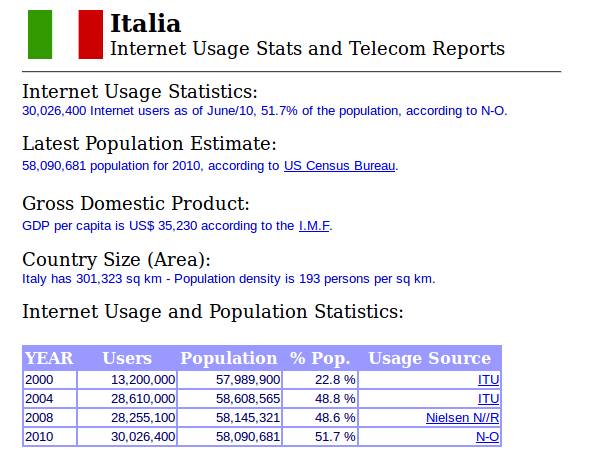
\includegraphics[scale=0.55]{images/cap1/statItaly} 
\end{figure}

Inoltre, l'interfaccia web sarà sviluppata tale da rimanere inalterata se visualizzata con diversi browser, anche con differenti versioni.\\
Riportiamo di seguito le statistiche percentuali sull'utilizzo dei browser aggiornate a giugno 2012.

\begin{figure}[H]
\centering
\caption{Statistiche ufficiali Api}
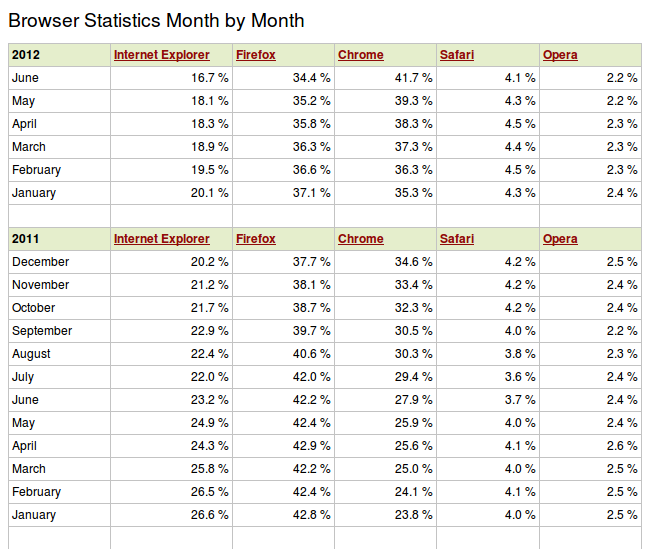
\includegraphics[scale=0.55]{images/cap1/internetStat} 
\end{figure}


\subsubsection{Client Mobile}
Per ogni dispositivo è disponibile un client distribuito a seconda della piattaforma in uso.\\
Dopo la canonica inizializzazione e assegnazione di un account da parte del Super-user, lo User può direttamente autenticarsi e cominciare a operare tramite l’interfaccia dell’applicazione.\\ 
Un Mobile-user ha inoltre la facoltà di agire esattamente come un Desktop-user tramite l’interfaccia web.\\
Dopo un'attenta valutazione e in base ai criteri di seguito esposti, abbiamo deciso di sviluppare l'applicazione solo su dispositivi Android, data la limitazione derivante dalle risorse concesse.\\
Nulla vieta, in futuro, di poter sviluppare l'applicazione anche per diversi sistemi.

\begin{figure}[H]
\centering
\caption{Statistiche d'uso dispositivi Android}
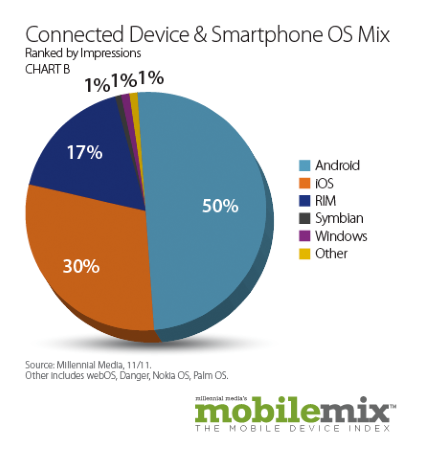
\includegraphics[scale=0.50]{images/cap1/statAndroid} 
\end{figure}

Per quanto riguarda la scelta della versione da utilizzare abbiamo seguite le seguenti statistiche; gli aspetti tecnici tuttavia verranno trattati più dettagliatamente nei prossimi capitoli.\\

\begin{figure}[H]
\centering
\caption{Statistiche ufficiali Api}
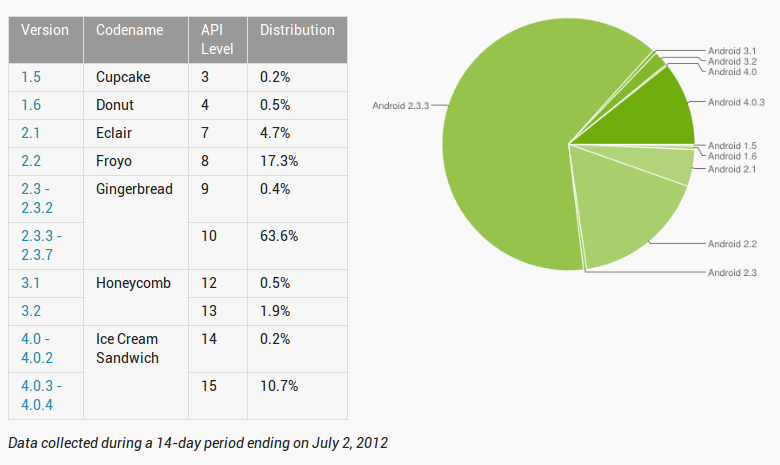
\includegraphics[scale=0.55]{images/cap1/api} 
\end{figure}

\newpage

\subsection{Caratteristiche degli utenti}
Gli attori chiamati in causa si suddivideranno nelle seguenti categorie:

\begin{enumerate}

\item Woty Administrator\\
L'attività assegnata al Woty Administrator è quella di illustrare il funzionamento del software presso il cliente ed eventualmente aiutare ad installare le applicazioni mobile.\\
E' incaricato dell'inserimento delle quest. Conoscenze pratiche richieste: gestione di sistemi e reti informatiche.\\

\item Desktop-user, a loro volta divisi in:

\begin{enumerate}

\item Desktop-user senza dispositivo mobile\\
Questo tipo di attore dovrà svolgere le varie quest assegnategli da postazione fissa;

\item Desktop-user con dispositivo mobile\\
Questo tipo di attore dovrà svolgere le varie quest assegnategli, inoltre potrà averne a disposizione altre specifiche in cui si richiede l'uso di un dispositivo mobile (e.g. rilevamento di QR-Code).

\end{enumerate}

\item Mobile-user\\
Questa tipologia di utenti potrà svolgere le proprie quest direttamente dal dispositivo mobile, quindi senza essere fisicamente nell'azienda.

\paragraph{}
Per entrambi gli attori Desktop-user e Mobile-user non sono richieste particolari conoscenze informatiche.

\item Super-user\\
Il Super-user sarà colui che all'interno dell'azienda dovrà occuparsi di visionare i risultati delle varie quest ed eventualmente illustrarne il funzionamento agli User. Si occupa inoltre dell'assegnazione di workgroup agli User del sistema.

\end{enumerate}

\newpage

\subsection{Descrizione quest}

Le tipologie di quest che un User può sostenere sono varie, caratterizzate da un input che Woty darà all'utente e da una risposta che l'utente darà al sistema, in base alle richieste.\\
SevenFold si riserva di ampliare e/o modificare le tipologie di quest offerte durante lo sviluppo di Woty, a seguito di decisioni prese in sinergia con la ditta proponente.\\

\subsubsection{Caratterizzazione in base all'input Woty -> User}
\begin{itemize}
\item Testo: l'User visualizzerà un semplice testo.
\item Foto: l'User visualizzerà a video un'immagine.
\item Video: l'User visualizzerà un filmato.
\end{itemize}

\subsubsection{Caratterizzazione in base alla risposta dell'User}
\begin{itemize}
\item Risposta secca (si/no, vero/falso)
\item Risposta chiusa tra un certo numero alternative
\item Risposta multipla tra un certo numero di opzioni
\item In caso di quest basata su testi, possibilità di riordinare testi disordinati
\item In caso di quest basata su foto, possibilità di riordinare foto spezzettata e disordinata (puzzle)
\item Scansione di un QR-Code$^g$ (Mobile-user)
\end{itemize}

\subsubsection{Caratterizzazione in base al tempo di risoluzione}
\begin{itemize}
\item Standard: quest senza un limite di tempo di risoluzione.
\item Temporizzata: quest con un limite di tempo di risoluzione.
\end{itemize}


\comment{
\section{Use Case e descrizioni}

\thispagestyle{fancy}

Di seguito sono riportati gli Use Case (UC$^g$) relativi ai requisiti funzionali su cui si basa il sistema. Ogni diagramma UC sarà integrato con una spiegazione nella quale ne verranno indicati gli attori e i rispettivi scenari nei quali si possono trovare.\\
Gli use case vengono organizzati in forma gerarchica secondo la seguente classificazione:\\
La notazione utilizzata è la seguente:\\

Uc X<.Y<.Z> >\\

dove le seguenti sigle indicano:
\begin{itemize}
\item[\textbf{X:}] use case di primo livello
\item[\textbf{Y:}] use case di secondo livello
\item[\textbf{Z:}] use case di terzo livello\\
\end{itemize}
I campi Y e Z possono essere assenti.

\subsection{Gerarchia attori}
% inserire una figura
\begin{figure}[h]
\centering
\caption{Gerarchia attori}
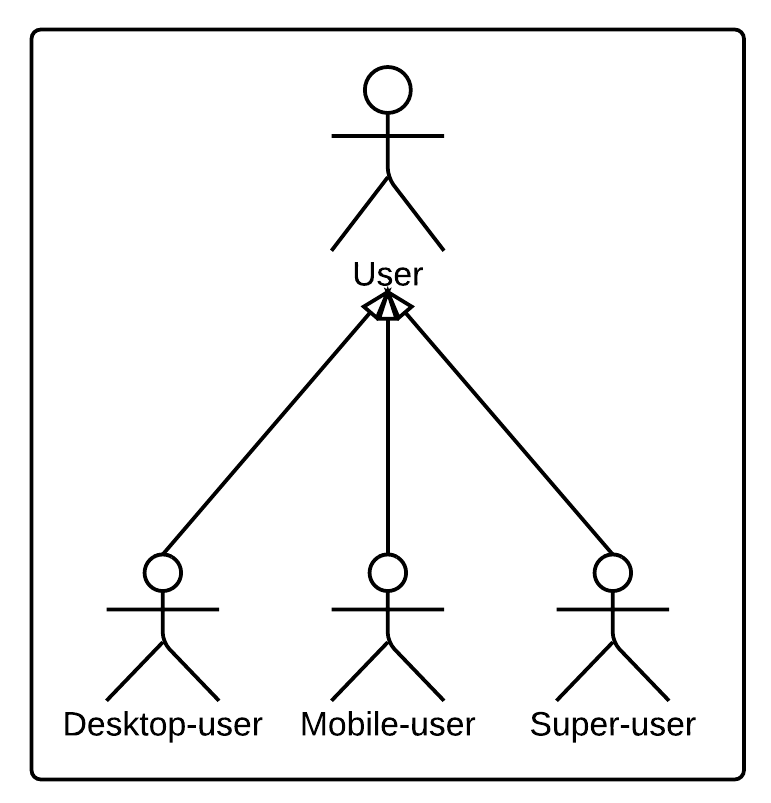
\includegraphics[scale=0.87]{images/cap1/UseCase/UcUser} % vedi Lateximpazienye pg67
\end{figure}

\begin{itemize}

\item \textbf{Attori coinvolti}:
\emph{- User}: utente generico del sistema.\\
\emph{- Desktop-user}: è uno User che interagisce con il sistema tramite con un computer fisso.\\
\emph{- Mobile-user}: è uno User che interagisce con il sistema tramite smartphone.\\
\emph{- Super-user}: è uno User con privilegi di amministrazione.\\
\emph{- PMAC Administrator}: amministratore PMAC.
\end{itemize}

\newpage

\subsection{Uc: PMAC}
% inserire una figura
\begin{figure}[ht]
\centering
\caption{Uc: PMAC}
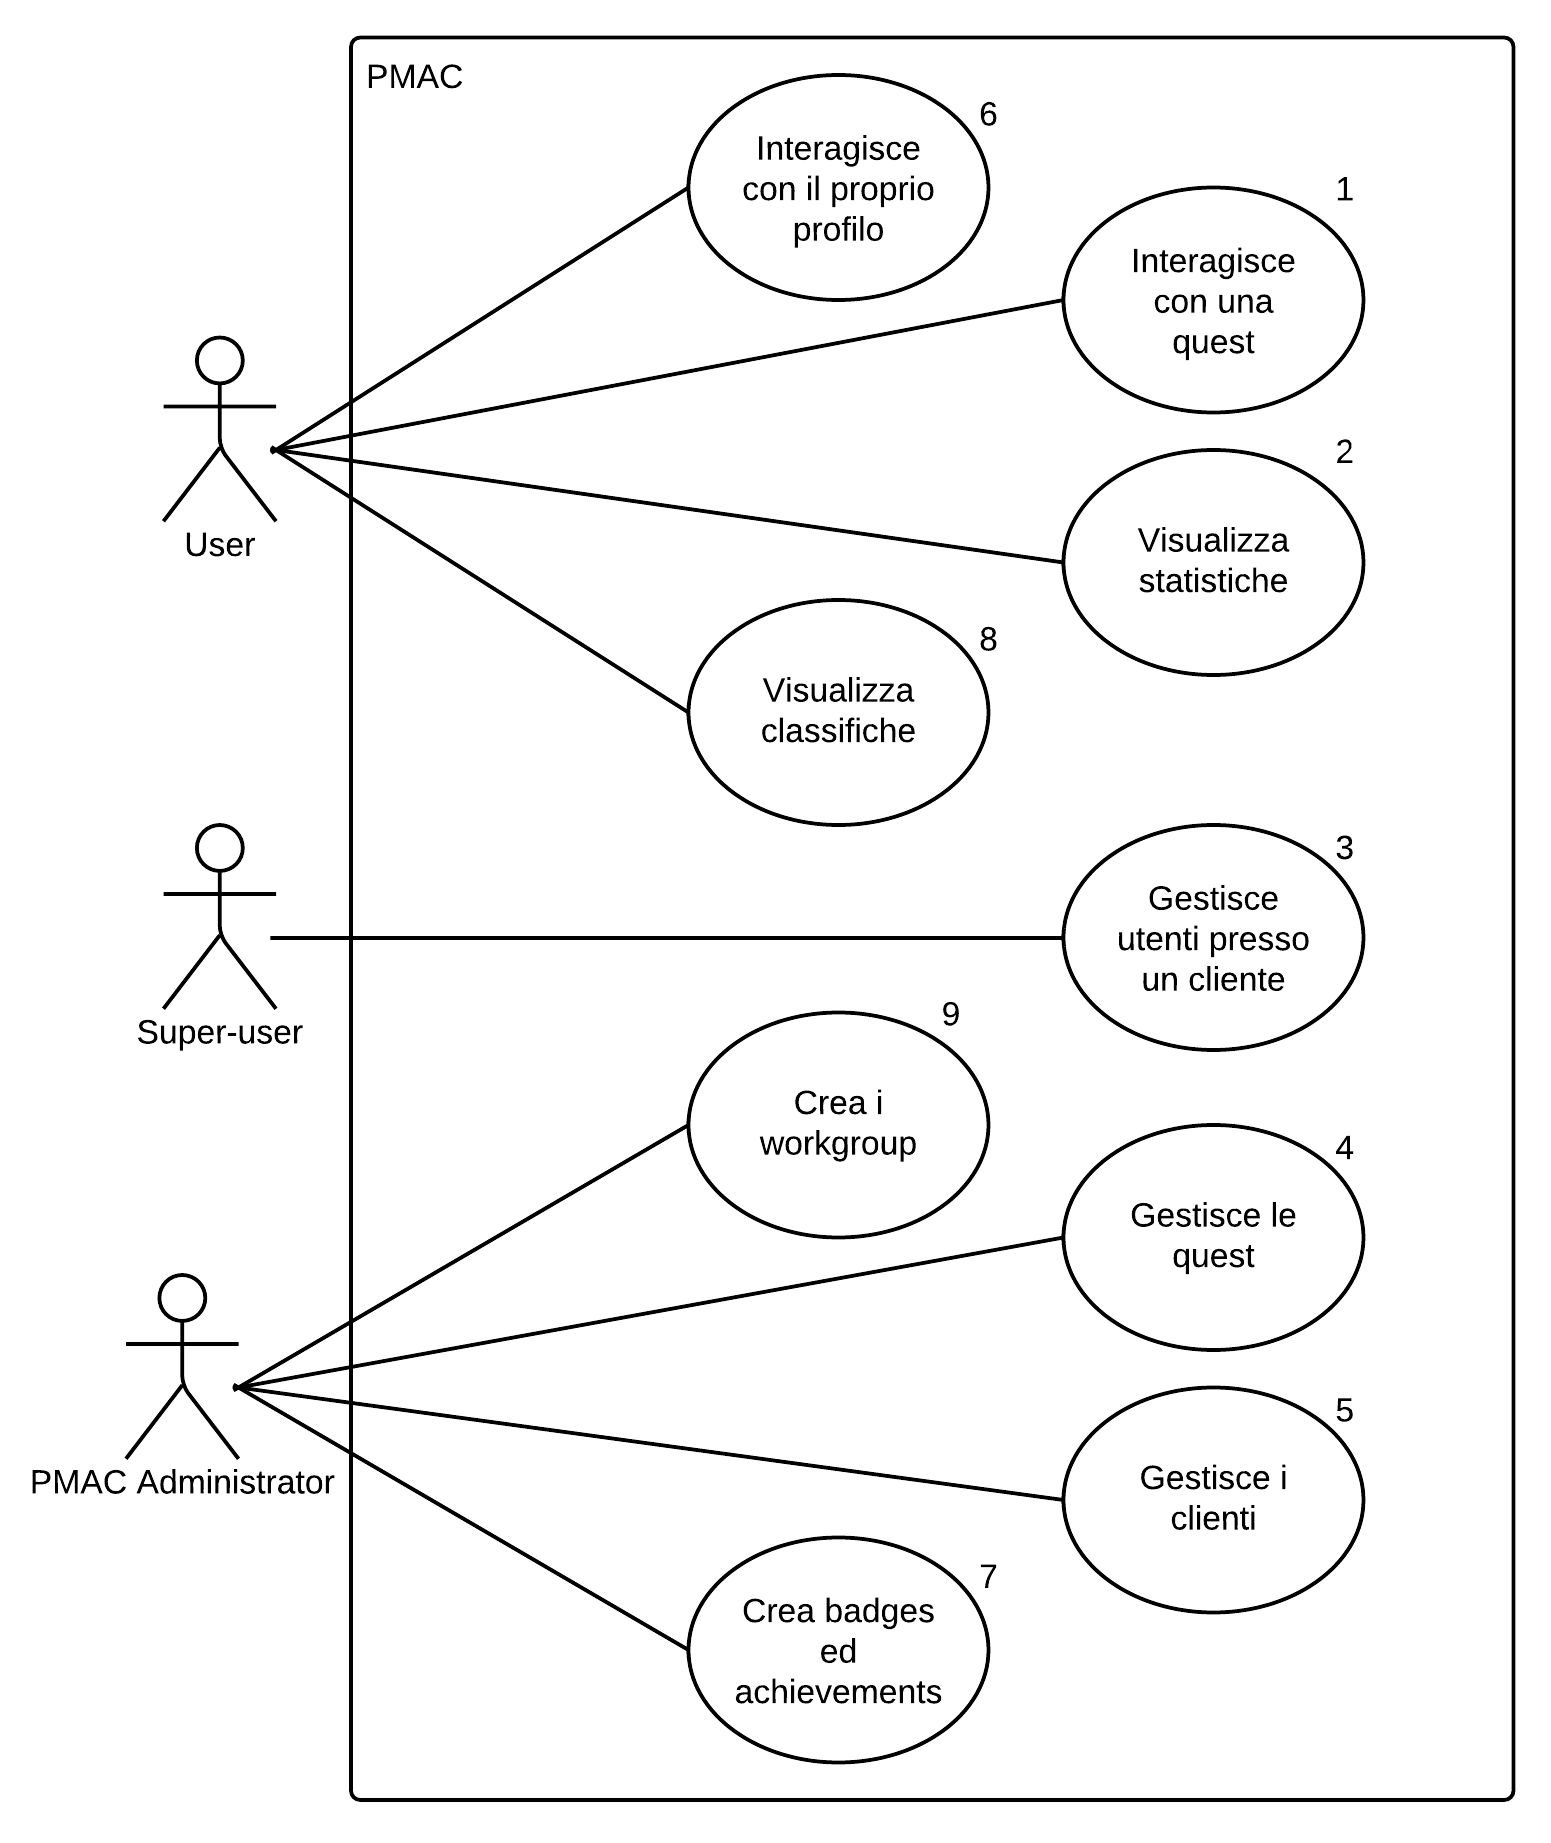
\includegraphics[scale=0.69]{images/cap1/UseCase/UcPMAC} % vedi Lateximpazienye pg67
\end{figure}

\begin{itemize}
\item \textbf{Attori coinvolti}:\\
\emph{- User}: utente generico del sistema.\\
\emph{- Desktop-user}: è uno User che interagisce con il sistema tramite con un computer fisso.\\
\emph{- Mobile-user}: è uno User che interagisce con il sistema tramite smartphone.\\
\emph{- Super-user}: è uno User con privilegi di amministrazione.\\
\emph{- PMAC Administrator}: amministratore PMAC.

\item \textbf{Precondizioni}:\\
L'attore che interagisce con il sistema deve possedere un account e deve aver effettuato l'accesso.

\item \textbf{Postcondizione}:\\
Interazione conclusa, sistema PMAC in stato stabile e pronto per una nuova interazione.

\item \textbf{Scenario principale}:\\
- User può interagire con una quest, quindi richiedere, ricevere, affrontare o rifiutare una quest inviatagli dal sistema. [Uc 1]\\
- User può visualizzare le proprie statistiche riguardo il completamento delle quest. [Uc 2]\\
- User può visualizzare le classifiche della gamification. [Uc 8]\\
- User può interagire con il proprio profilo, modificando e aggiornando i dati personali. [Uc 6]\\
- Super-user può gestire gli account degli utenti della sua azienda. [Uc 3]\\
- PMAC Administrator può creare nuovi workgroup, inserendo nuovi dipartimenti non ancora presenti alle quali assegnare determinate quest. [Uc 9]\\
- PMAC Administrator può gestire i clienti del sistema. [Uc 5]\\\\
- PMAC Administrator può gestire le quest con modifiche quali rimuovi, assegna e crea. [Uc 4]\\
- PMAC Administrator può creare i badge$^g$ e gli achievement$^g$. Eventuali informazioni sulla composizione di questi elementi della gamification saranno specificate nei requisiti relativi. [Uc 7]
\end{itemize}


\subsection{Uc 1: Interagisce con una quest}
% inserire una figura
\begin{figure}[ht]
\centering
\caption{Uc 1: Interagisce con una quest}
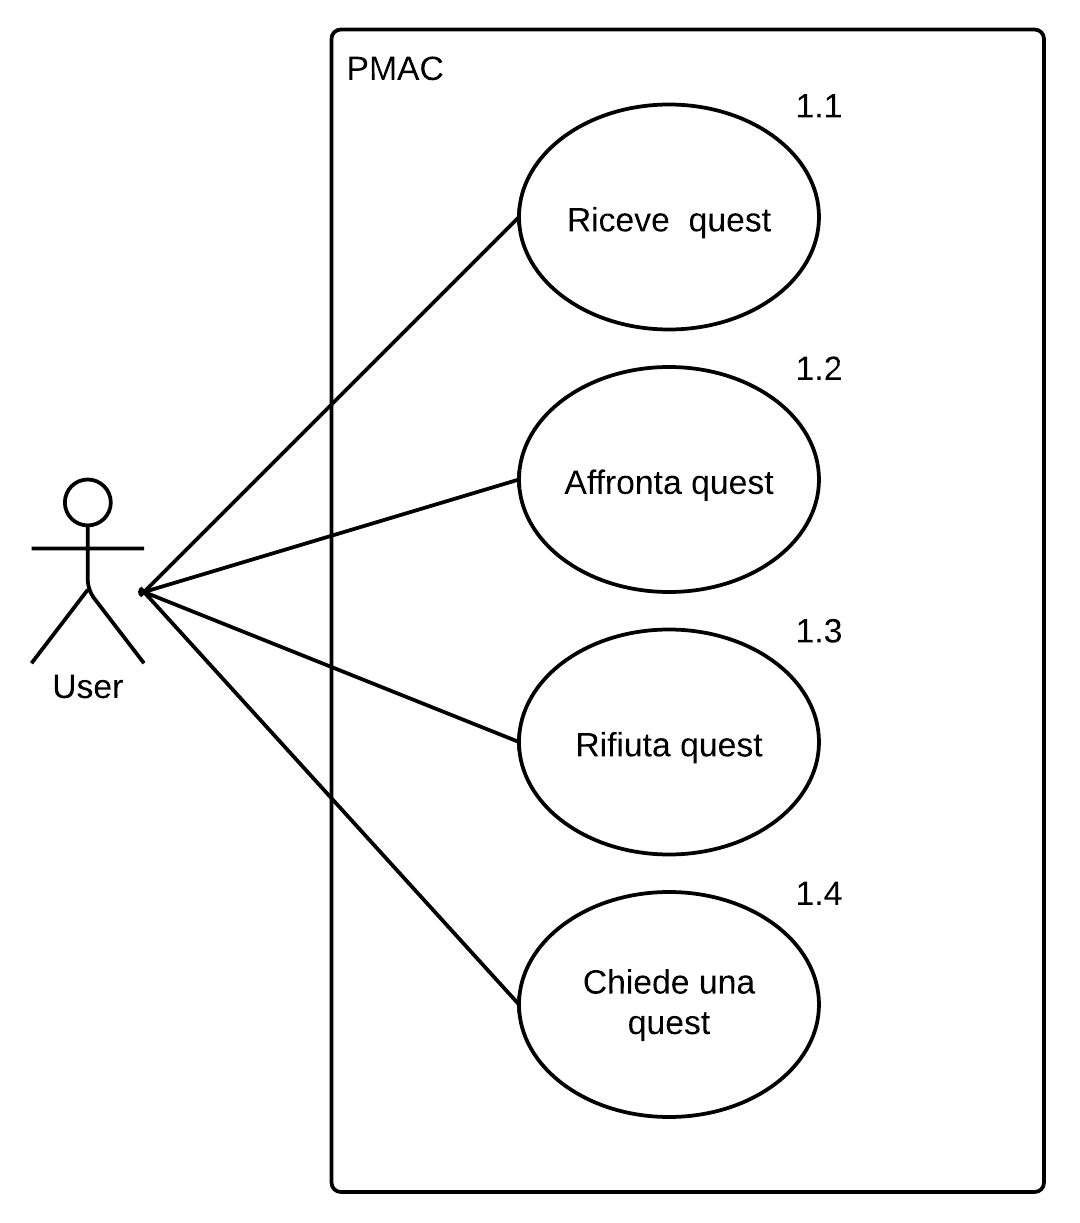
\includegraphics[scale=0.8]{images/cap1/UseCase/Uc1} % vedi Lateximpazienye pg67
\end{figure}

\begin{itemize}
\item \textbf{Attori coinvolti}:\\
\emph{- User: utente generico del sistema.}

\item \textbf{Precondizione:}\\
L'utente che interagisce con il sistema deve possedere un account e deve aver effettuato l'accesso.

\item \textbf{Postcondizione:}\\
L'utente ha interagito con una quest ed il sistema è pronto per una nuova interazione.

\item \textbf{Scenario principale:}\\
User può ricevere una quest inviatagli dal sistema e affrontarla tramite l'utilizzo del browser, oppure può ignorarla per svolgere regolarmente il suo lavoro. User può anche richiedere al sistema una nuova quest tramite l'utilizzo dell'apposita funzione nell'interfaccia grafica. [Uc 1.1, Uc 1.2, Uc 1.3 e Uc 1.4]
\end{itemize}
\newpage

\subsection{Uc 1.2: Affronta Quest}
% inserire una figura
\begin{figure}[ht]
\centering
\caption{Uc 1.2: Affronta quest}
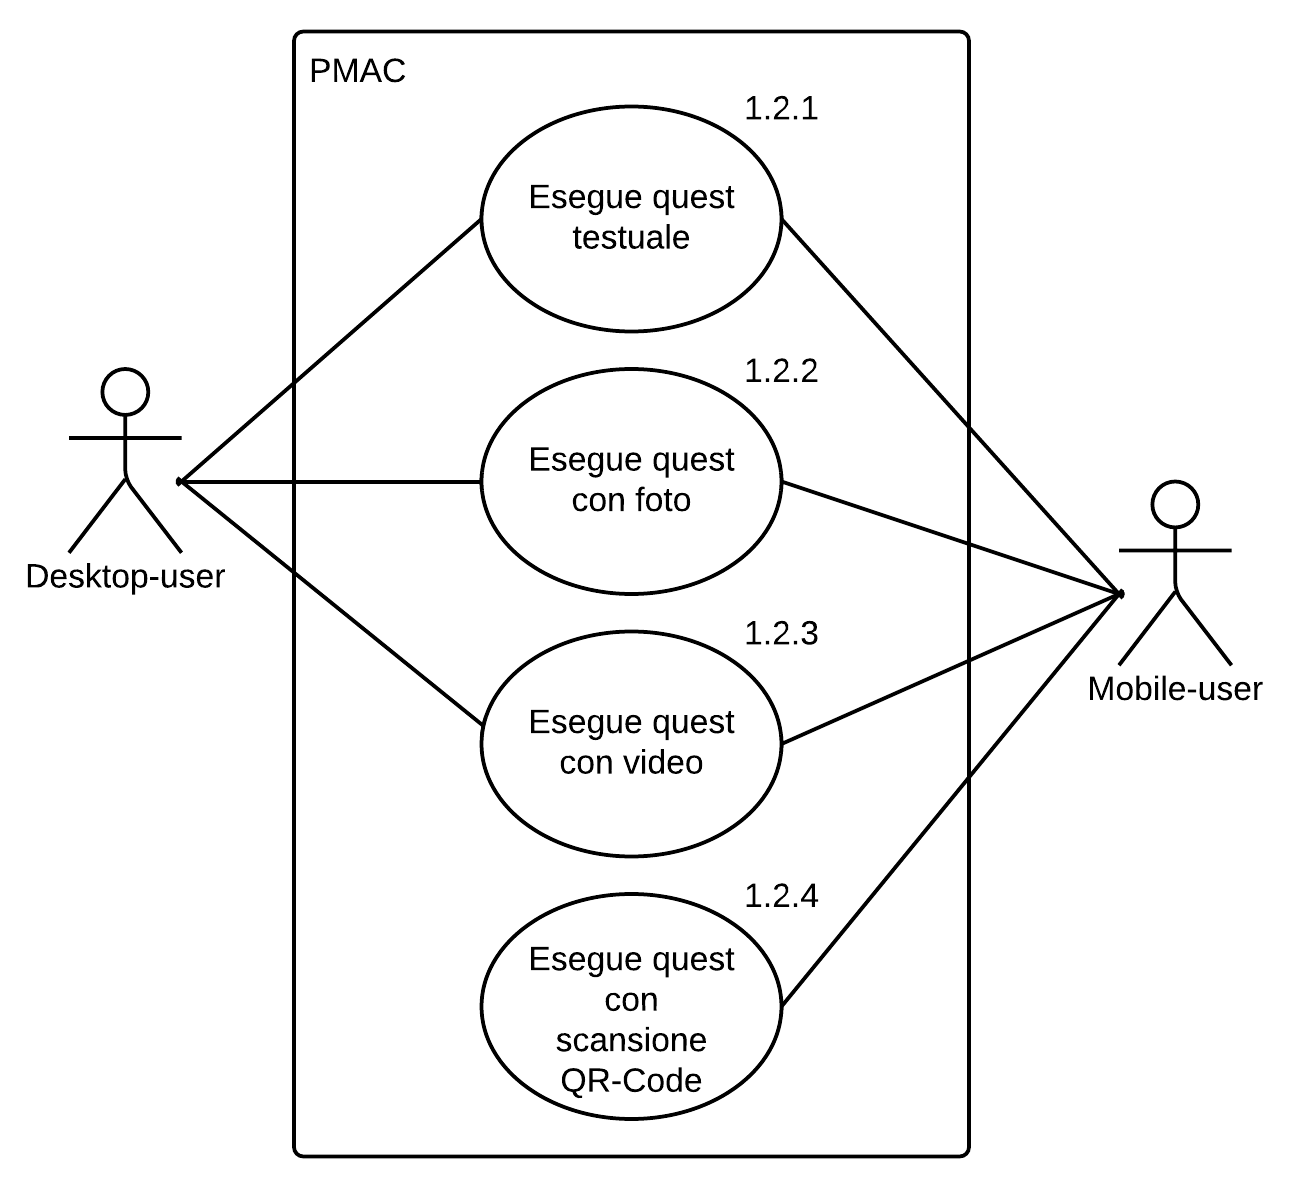
\includegraphics[scale=0.87]{images/cap1/UseCase/Uc1_2} % vedi Lateximpazienye pg67
\end{figure}

\begin{itemize}

\item \textbf{Attori coinvolti:}\\
\emph{- Desktop-user}: è uno User che interagisce con il sistema tramite con un computer fisso.\\
\emph{- Mobile-user}: è uno User che interagisce con il sistema tramite smartphone.

\item \textbf{Precondizione}:\\
L'attore che interagisce con il sistema deve possedere un account e deve aver effettuato l'accesso. Il sistema PMAC si trova nella pagina dedicata alla scelta della quest da svolgere.

\item \textbf{Postcondizione}:\\
L'utente ha eseguito la quest e il sistema PMAC è pronto per una nuova interazione e si trova alla pagina dedicata alla selezione della quest da svolgere dall'utente.

\item \textbf{Scenario principale}:\\
- Desktop-User può eseguire quest di tipo testuale, con foto e con video. [Uc 1.2.1 + Uc 1.2.2 + Uc 1.2.3]\\
- Mobile-user può eseguire tutte le tipologie di quest, comprese le quest con scansione di QR-Code. [Uc 1.2.1 + Uc 1.2.2 + Uc 1.2.3 + Uc 1.2.4]

\item \textbf{Scenario alternativo}:\\
L'utente decide di non rispondere alla quest avviata e il sistema torna alla pagina di selezione delle quest da svolgere. Questo scenario non è possibile per le quest temporizzate, le quali verranno segnalate all'utente nella pagine di selezione delle quest.

\end{itemize}

\newpage

\subsection{Uc 2: Visualizza statistiche}
% inserire una figura
\begin{figure}[ht]
\centering
\caption{Uc 2: Visualizza statistiche}
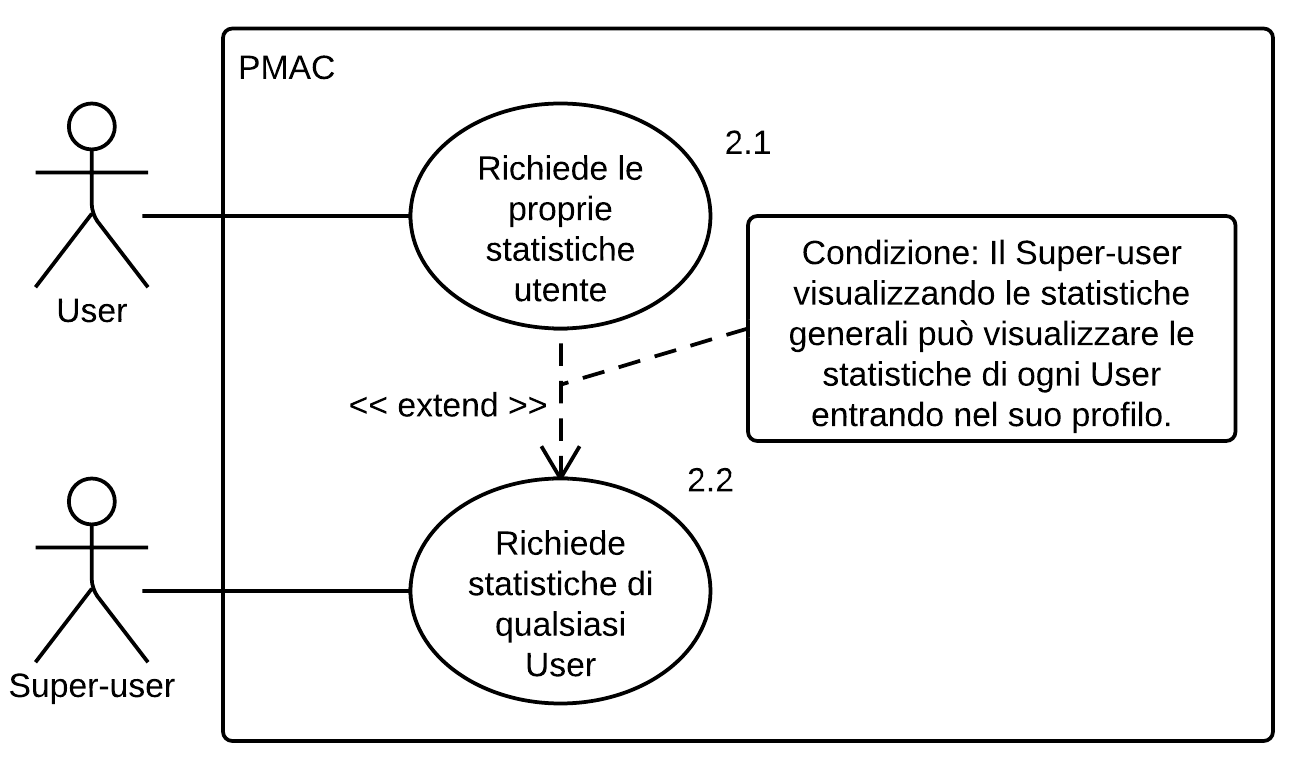
\includegraphics[scale=0.87]{images/cap1/UseCase/Uc2} % vedi Lateximpazienye pg67
\end{figure}

\begin{itemize}

\item \textbf{Attori coinvolti:}\\
\emph{- User}: utente generico del sistema.\\
\emph{- Super-user}: figura presso il cliente con privilegi di amministrazione.

\item \textbf{Precondizione}:\\
L'attore che interagisce con il sistema deve possedere un account e deve aver effettuato l'accesso.

\item \textbf{Postcondizione}:\\
Il sistema PMAC si trova nella pagina dedicata alla visualizzazione delle statistiche personali di uno User.

\item \textbf{Scenario principale}:\\
- User può visualizzare le proprie statistiche (punteggi, badge ed achievement). [Uc 2.1]\\
- Super-user può vedere tutte le classifiche ed entrando nel profilo di un utente può visualizzare i punteggi i badge e gli achievement di quell'utente. [Uc 2.2]
\end{itemize}

\newpage

\subsection{Uc 2.1: Richiede le proprie statistiche utente}
% inserire una figura
\begin{figure}[ht]
\centering
\caption{Uc 2.1: Richiede le proprie statistiche utente}
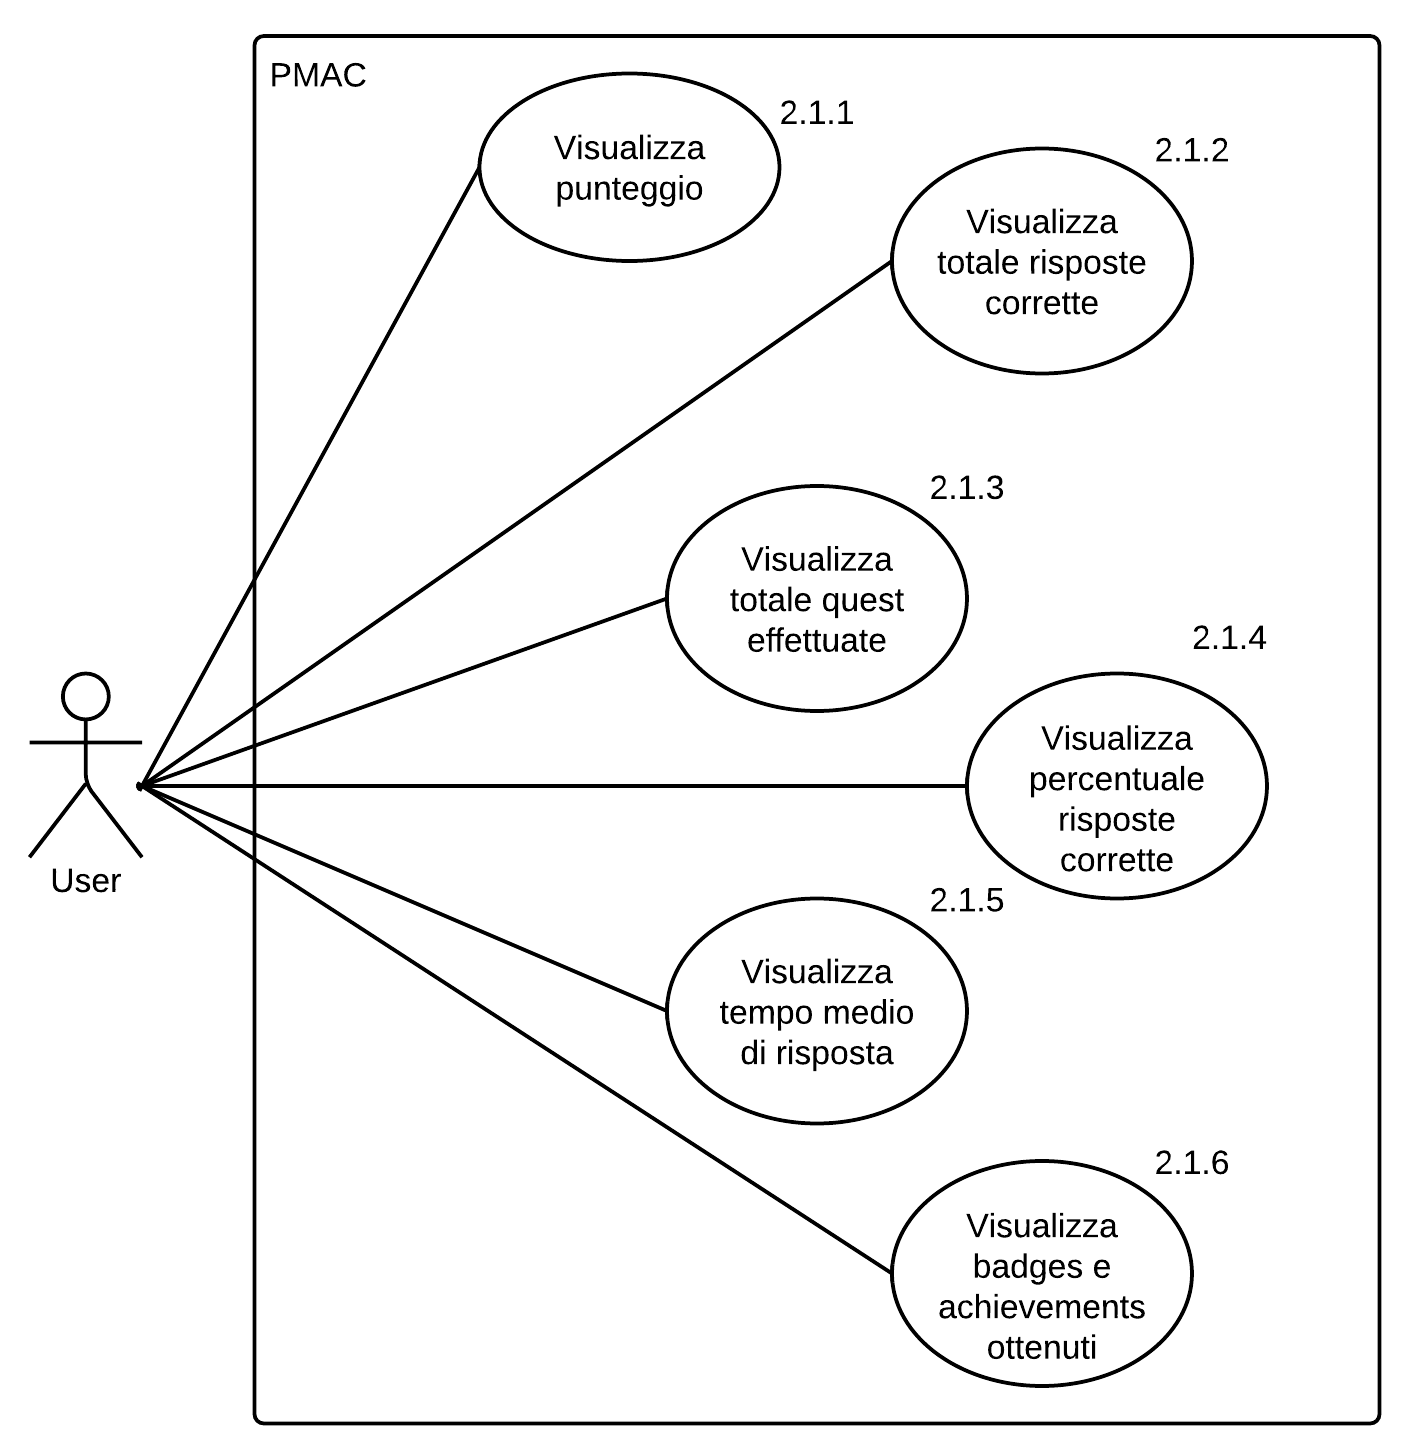
\includegraphics[scale=0.87]{images/cap1/UseCase/Uc2_1} % vedi Lateximpazienye pg67
\end{figure}

\begin{itemize}

\item \textbf{Attori coinvolti:}\\
\emph{- User}: utente generico del sistema.

\item \textbf{Precondizione}:\\
L'attore che interagisce con il sistema deve possedere un account e deve aver effettuato l'accesso. Il sistema PMAC si trova nella pagina dedicata alla visualizzazione delle statistiche personali dell'utente.

\item \textbf{Postcondizione}:\\
Le statistiche sono state visualizzate correttamente e il sistema rimane in attesa di una nuova interazione da parte dell'utente.

\item \textbf{Scenario principale}:\\
- User può visualizzare il proprio punteggio totale ricavato dalle risposte alle quest. [Uc 2.1.1]\\
- User può visualizzare il numero totale di risposte corrette effettuate.[Uc 2.1.2]\\
- User può visualizzare il numero totale di quest effettuate.[Uc 2.1.3]\\
- User può visualizzare la percentuale di risposte corrette rispetto al totale di quest effettuate.[Uc 2.1.4]\\
- User può visualizzare il proprio tempo medio di risposta alle quest. [Uc 2.1.5]\\
- User può visualizzare i propri badges e achievements.[Uc 2.1.6]
\end{itemize}

\newpage

\subsection{Uc 3: Gestisce utenti}
% inserire una figura
\begin{figure}[ht]
\centering
\caption{Uc 3: Gestisce utenti}
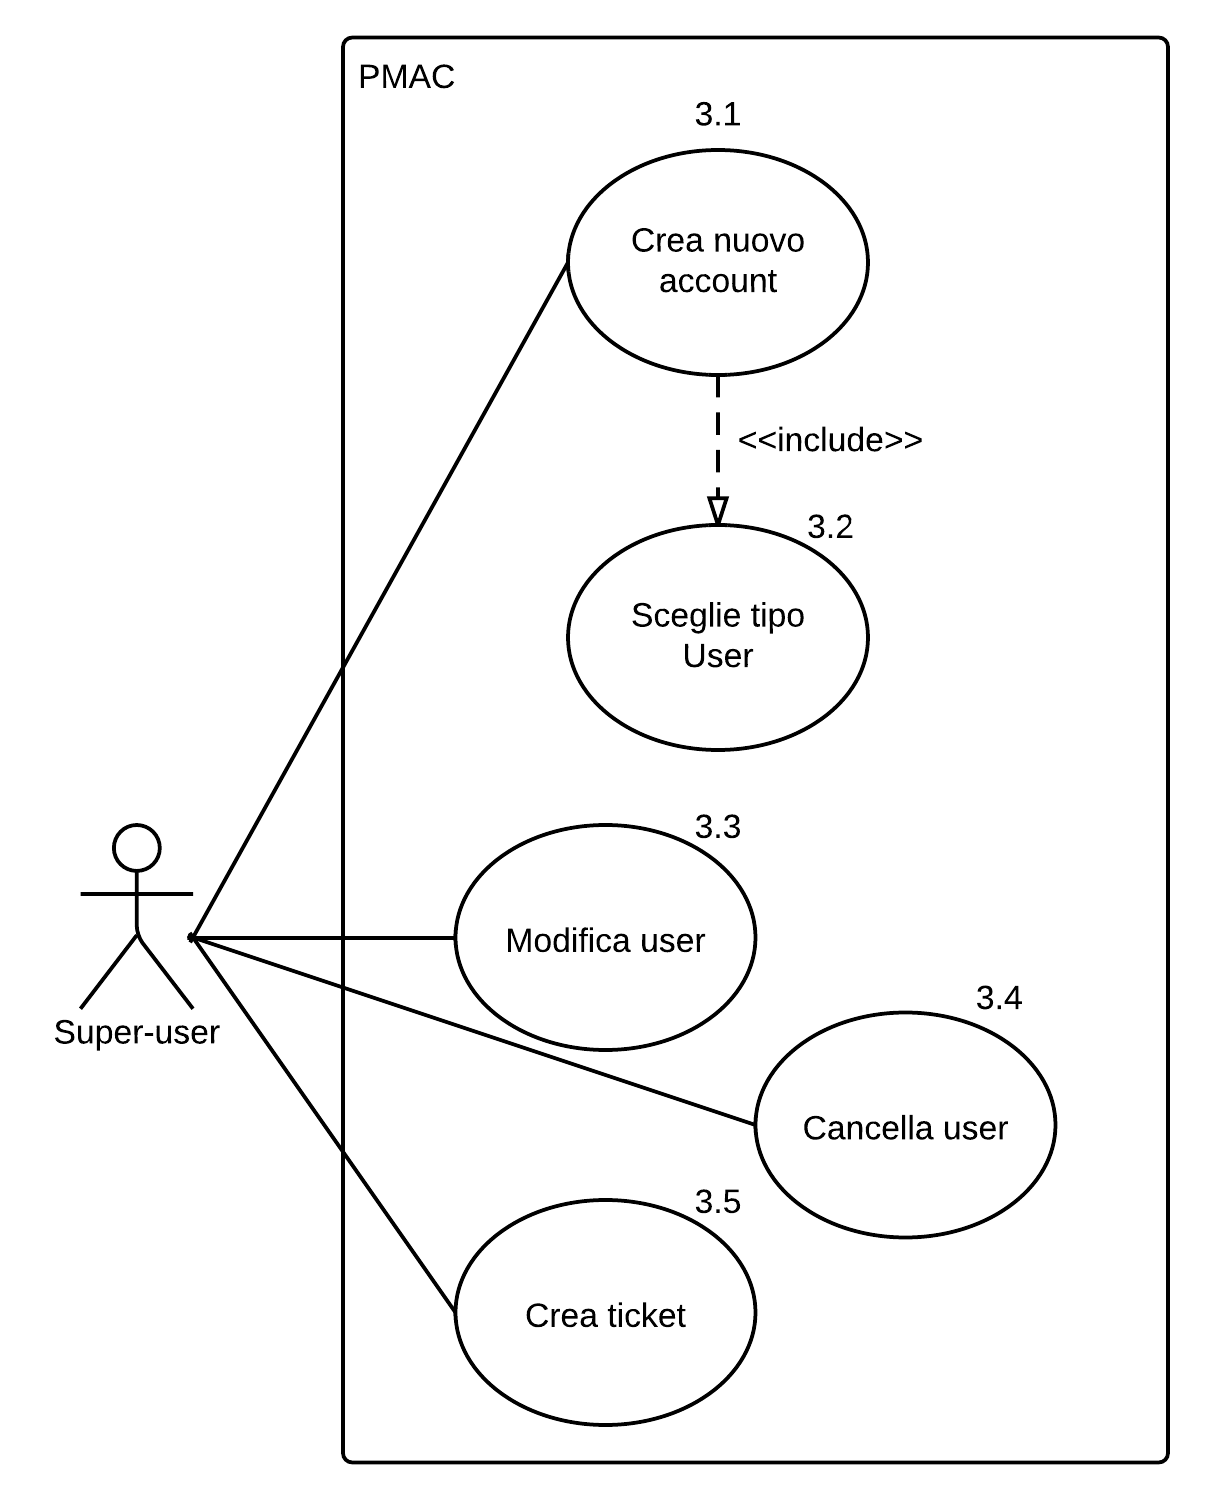
\includegraphics[scale=0.9]{images/cap1/UseCase/Uc3} % vedi Lateximpazienye pg67
\end{figure}

\begin{itemize}

\item \textbf{Attori coinvolti}:\\
\emph{- Super-user}: figura presso il cliente con privilegi di amministrazione.

\item \textbf{Precondizione}:\\
Il Super-user deve possedere un account e deve aver effettuato l'accesso al sistema. Il sistema si trova nella pagina principale dedicata al Super-user.

\item \textbf{Postcondizione}:\\
Le azioni effettuate sugli User sono state salvate correttamente dal sistema e i ticket creati sono stati inoltrati.

\item \textbf{Scenario principale}:\\
- Super-user può creare un nuovo account inserendo i suoi campi dati, specificando il tipo di User tra Desktop-user e Mobile-user. [Uc 3.1 + Uc 3.2]\\
- Super-user può modificare l'account di uno User cambiando i suoi dati personali e il tipo di account che possiede. [Uc 3.3]\\
- Super-user può cancellare uno User dal sistema. [Uc 3.4]\\
- Super-user può fare una richiesta testuale di modifica del contratto o di gestione degli account tramite la creazione di un ticket grazie all'interfaccia grafica. [Uc 3.5]
\end{itemize}

\newpage

\subsection{Uc 3.1: Crea un nuovo User account}
% inserire una figura
\begin{figure}[ht]
\centering
\caption{Uc 3.1: Crea un nuovo User account}
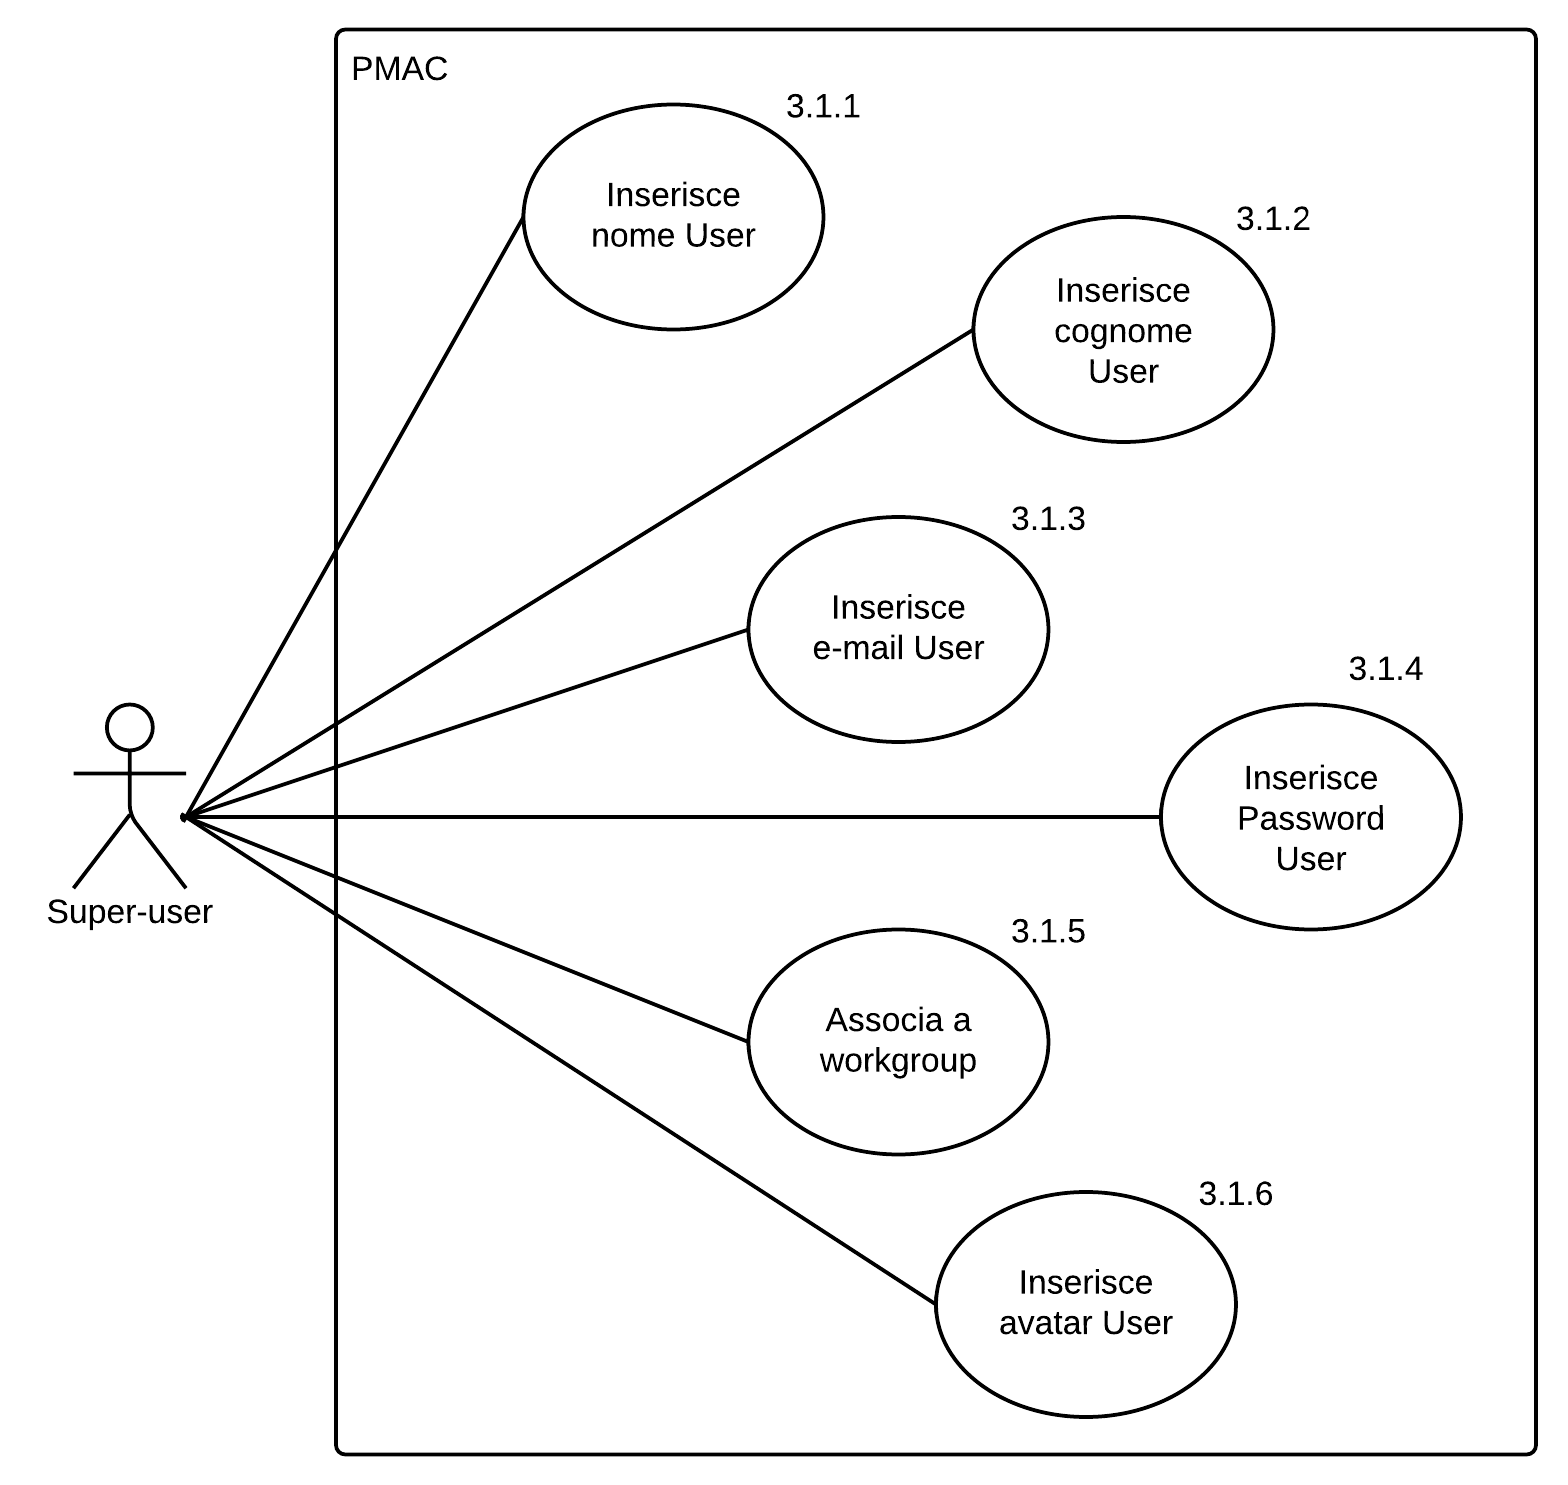
\includegraphics[scale=0.9]{images/cap1/UseCase/Uc3_1} % vedi Lateximpazienye pg67
\end{figure}

\begin{itemize}
\item \textbf{Attori coinvolti}:\\
\emph{- Super-user}: figura presso il cliente con privilegi di amministrazione.

\item \textbf{Precondizione}:\\
Il Super-user deve possedere un account e deve aver effettuato l'accesso al sistema. Il sistema si trova nella pagina dedicata all'inserimento di un nuovo User.

\item \textbf{Postcondizione}:\\
Il nuovo User è stato creato e inserito correttamente nel sistema. Il sistema si trova nella pagina principale dedicata al Super-user.

\item \textbf{Scenario principale}:\\
- Super-user può inserire il nome e il cognome del nuovo User. [Uc 3.1.1 + Uc 3.1.2]\\
- Super-user può inserire l'indirizzo e-mail del nuovo User, che verrà poi utilizzato dallo stesso come username nel login. [Uc 3.1.3]\\
- Super-user può inserire una password per il nuovo User. [Uc 3.1.4]\\
- Super-user può associare il nuovo User ad uno dei workgroup assegnati all'azienda. [Uc 3.1.5]\\
- Super-user può inserire un'immagine che fungerà da avatar per il nuovo User. [Uc 3.1.6]

\item \textbf{Scenario alternativo}:\\
Il Super-user inserisce un nuovo User con indirizzo email già occupato o non valido. Il sistema segnala l'errore e ripropone la schermata dedicata all'inserimento di un nuovo User.

\end{itemize}

\newpage

\subsection{Uc 3.3: Modifica uno User}
% inserire una figura
\begin{figure}[ht]
\centering
\caption{Uc 3.3: Modifica uno User}
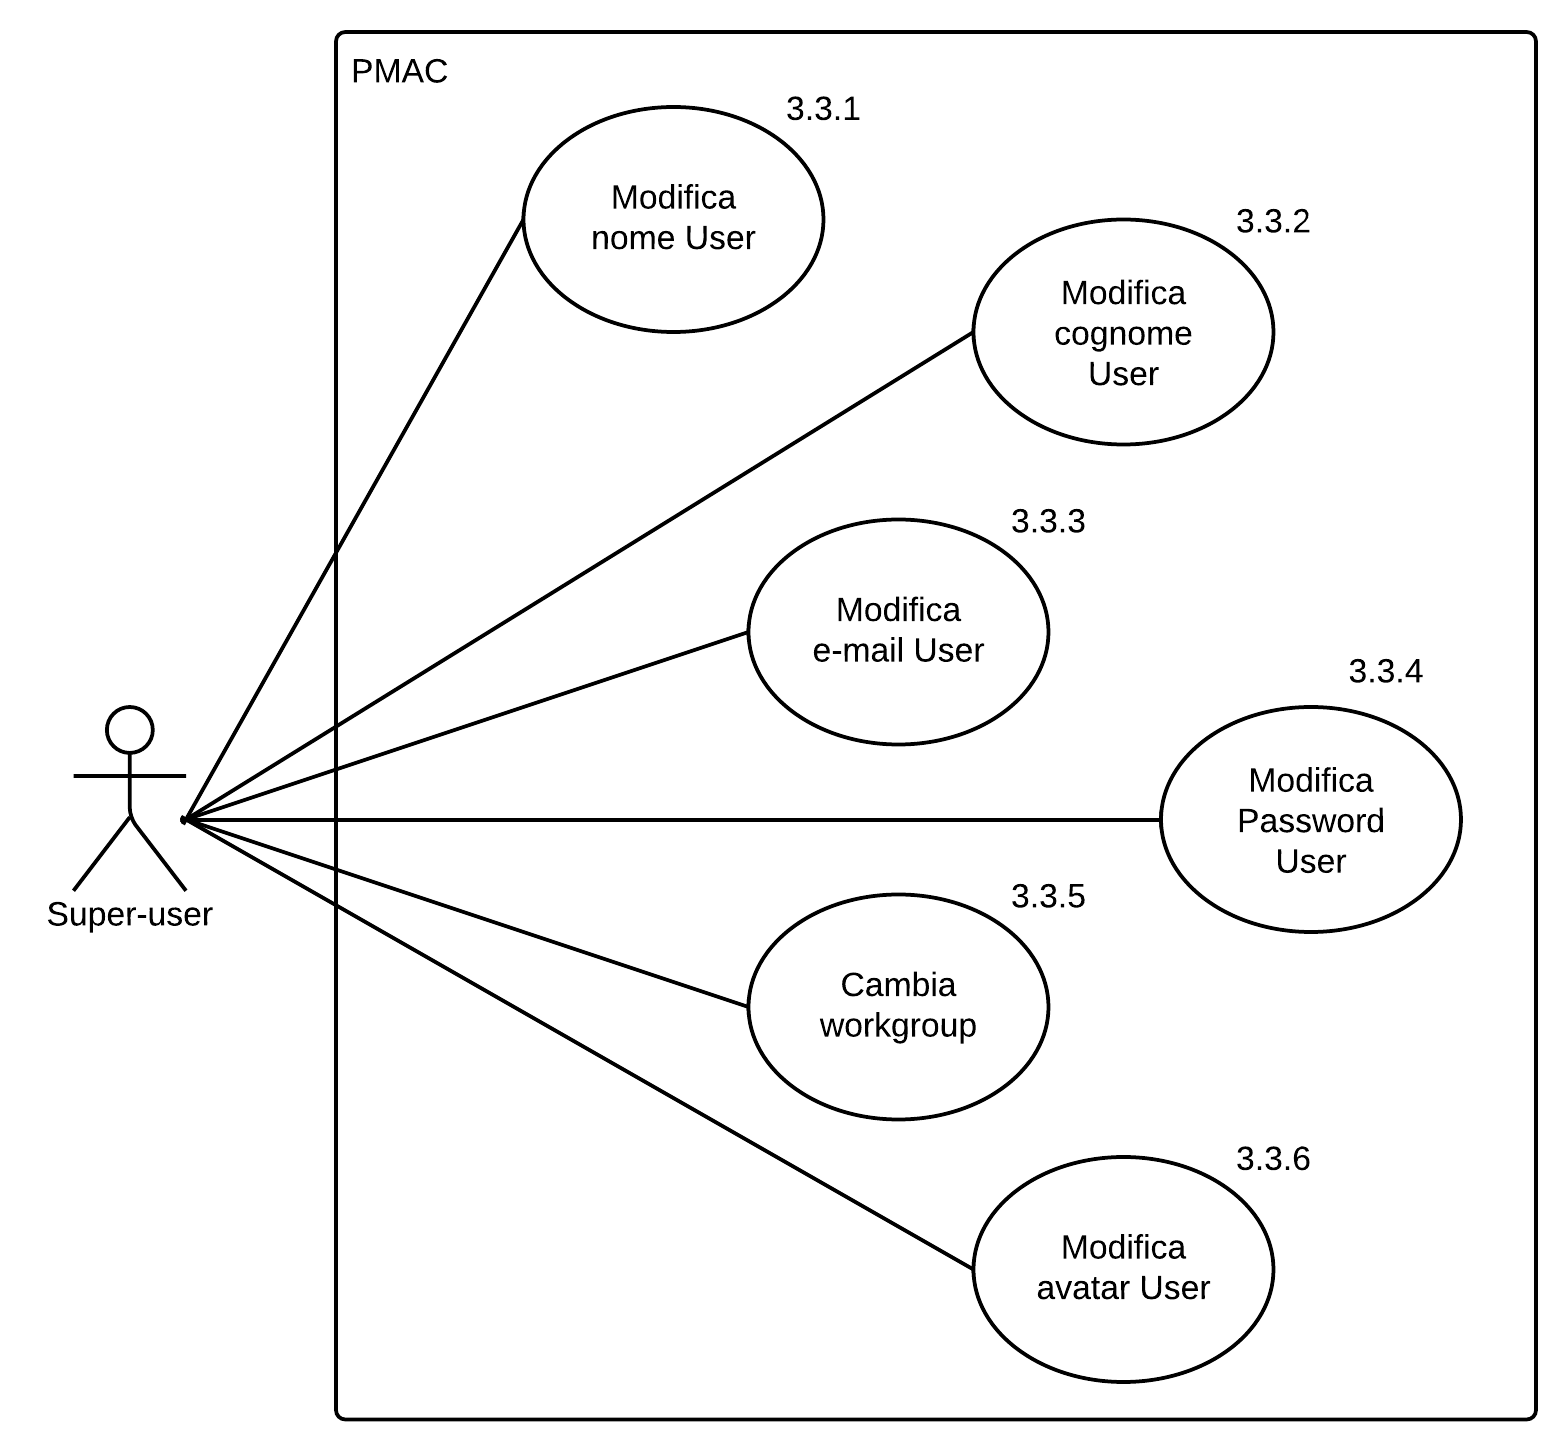
\includegraphics[scale=0.9]{images/cap1/UseCase/Uc3_3} % vedi Lateximpazienye pg67
\end{figure}

\begin{itemize}
\item \textbf{Attori coinvolti}:\\
\emph{- Super-user}: figura presso il cliente con privilegi di amministrazione.

\item \textbf{Precondizione}:\\
Il Super-user deve possedere un account e deve aver effettuato l'accesso al sistema. Il sistema si trova nella pagina dedicata alla modifica di uno User.

\item \textbf{Postcondizione}:\\
Lo User è stato modificato e le modifiche sono state salvate correttamente nel sistema. Il sistema si trova nella pagina principale dedicata al Super-user.

\item \textbf{Scenario principale}:\\
- Super-user può modificare il nome o il cognome dello User. [Uc 3.3.1 + Uc 3.3.2]\\
- Super-user può modificare l'indirizzo e-mail dello User, che verrà poi utilizzato dallo stesso come nuovo username nel login. [Uc 3.3.3]\\
- Super-user può modificare la password dello User. [Uc 3.3.4]\\
- Super-user può modificare il workgroup associato allo User. [Uc 3.3.5]\\
- Super-user può modificare l'avatar dello User. [Uc 3.3.6]\\
- Super-user può assegnare dei badges allo User. [Uc 3.3.7]

\item \textbf{Scenario alternativo}:\\
Il Super-user sostituisce l'indirizzo email di uno User con uno già occupato o non valido. Il sistema segnala l'errore e ripropone la schermata dedicata alla modifica dello User.

\end{itemize}

\newpage

\subsection{Uc 4: Gestisce le quest}
% inserire una figura
\begin{figure}[ht]
\centering
\caption{Uc 4: Gestisce le quest}
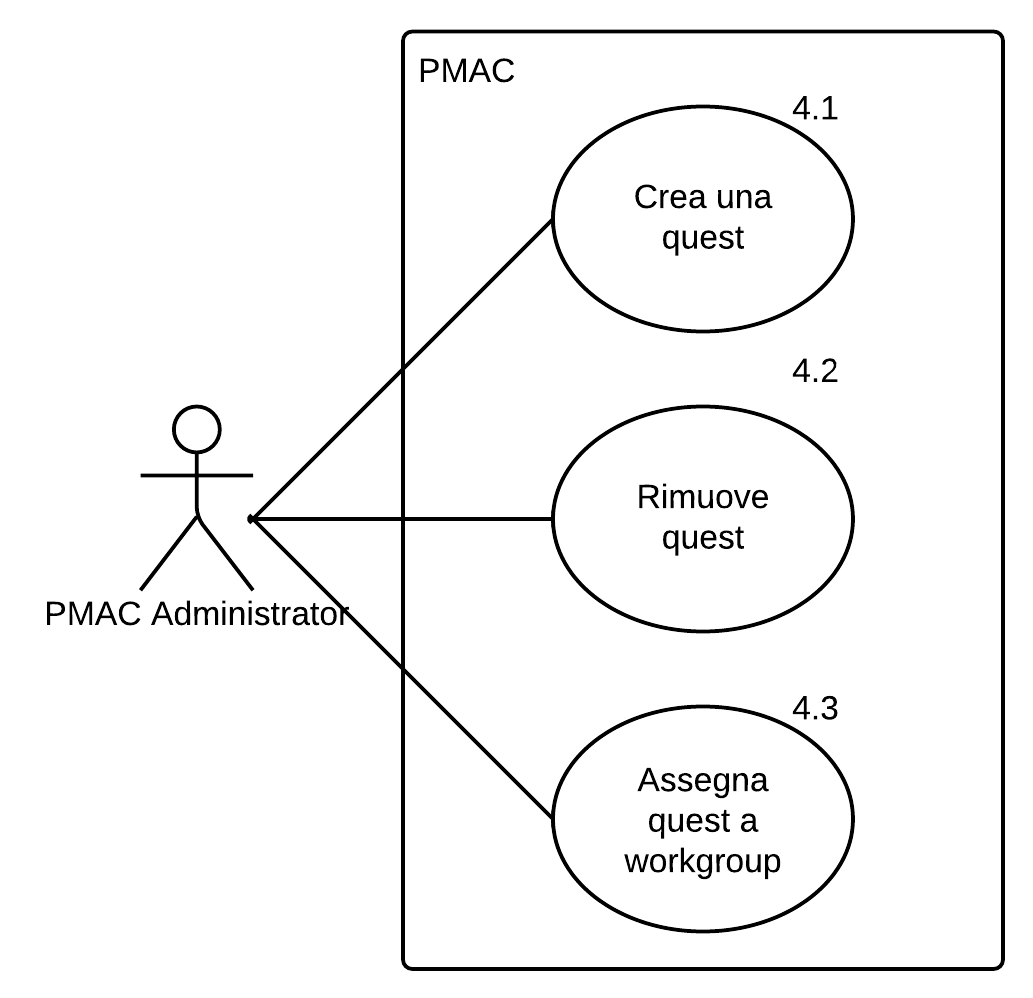
\includegraphics[scale=0.9]{images/cap1/UseCase/Uc4} % vedi Lateximpazienye pg67
\end{figure}

\begin{itemize}
\item \textbf{Attori coinvolti}:\\
\emph{- PMAC Administrator}: amministratore PMAC.

\item \textbf{Precondizione}:\\
PMAC Administrator deve possedere un account e deve aver effettuato l'accesso al sistema. Il sistema si trova nella pagina dedicata alla gestione delle quest.

\item \textbf{Postcondizione}:\\
Le quest sono state cancellate o caricate nel sistema PMAC e assegnate correttamente ai workgroup. Il sistema si trova nella pagina dedicata alla gestione delle quest.

\item \textbf{Scenario principale}:\\
- PMAC Administrator può creare una nuova quest per ampliare il database$^g$ usato per la gamification. [Uc 4.1]\\
- PMAC Administrator può rimuovere una quest dal sistema. [Uc 4.2]\\
- PMAC Administrator può assegnare una quest ad un workgroup. [Uc 4.3]
\end{itemize}

\newpage

\subsection{Uc 4.1: Crea una quest}
% inserire una figura
\begin{figure}[ht]
\centering
\caption{Uc 4.1: Crea una quest}
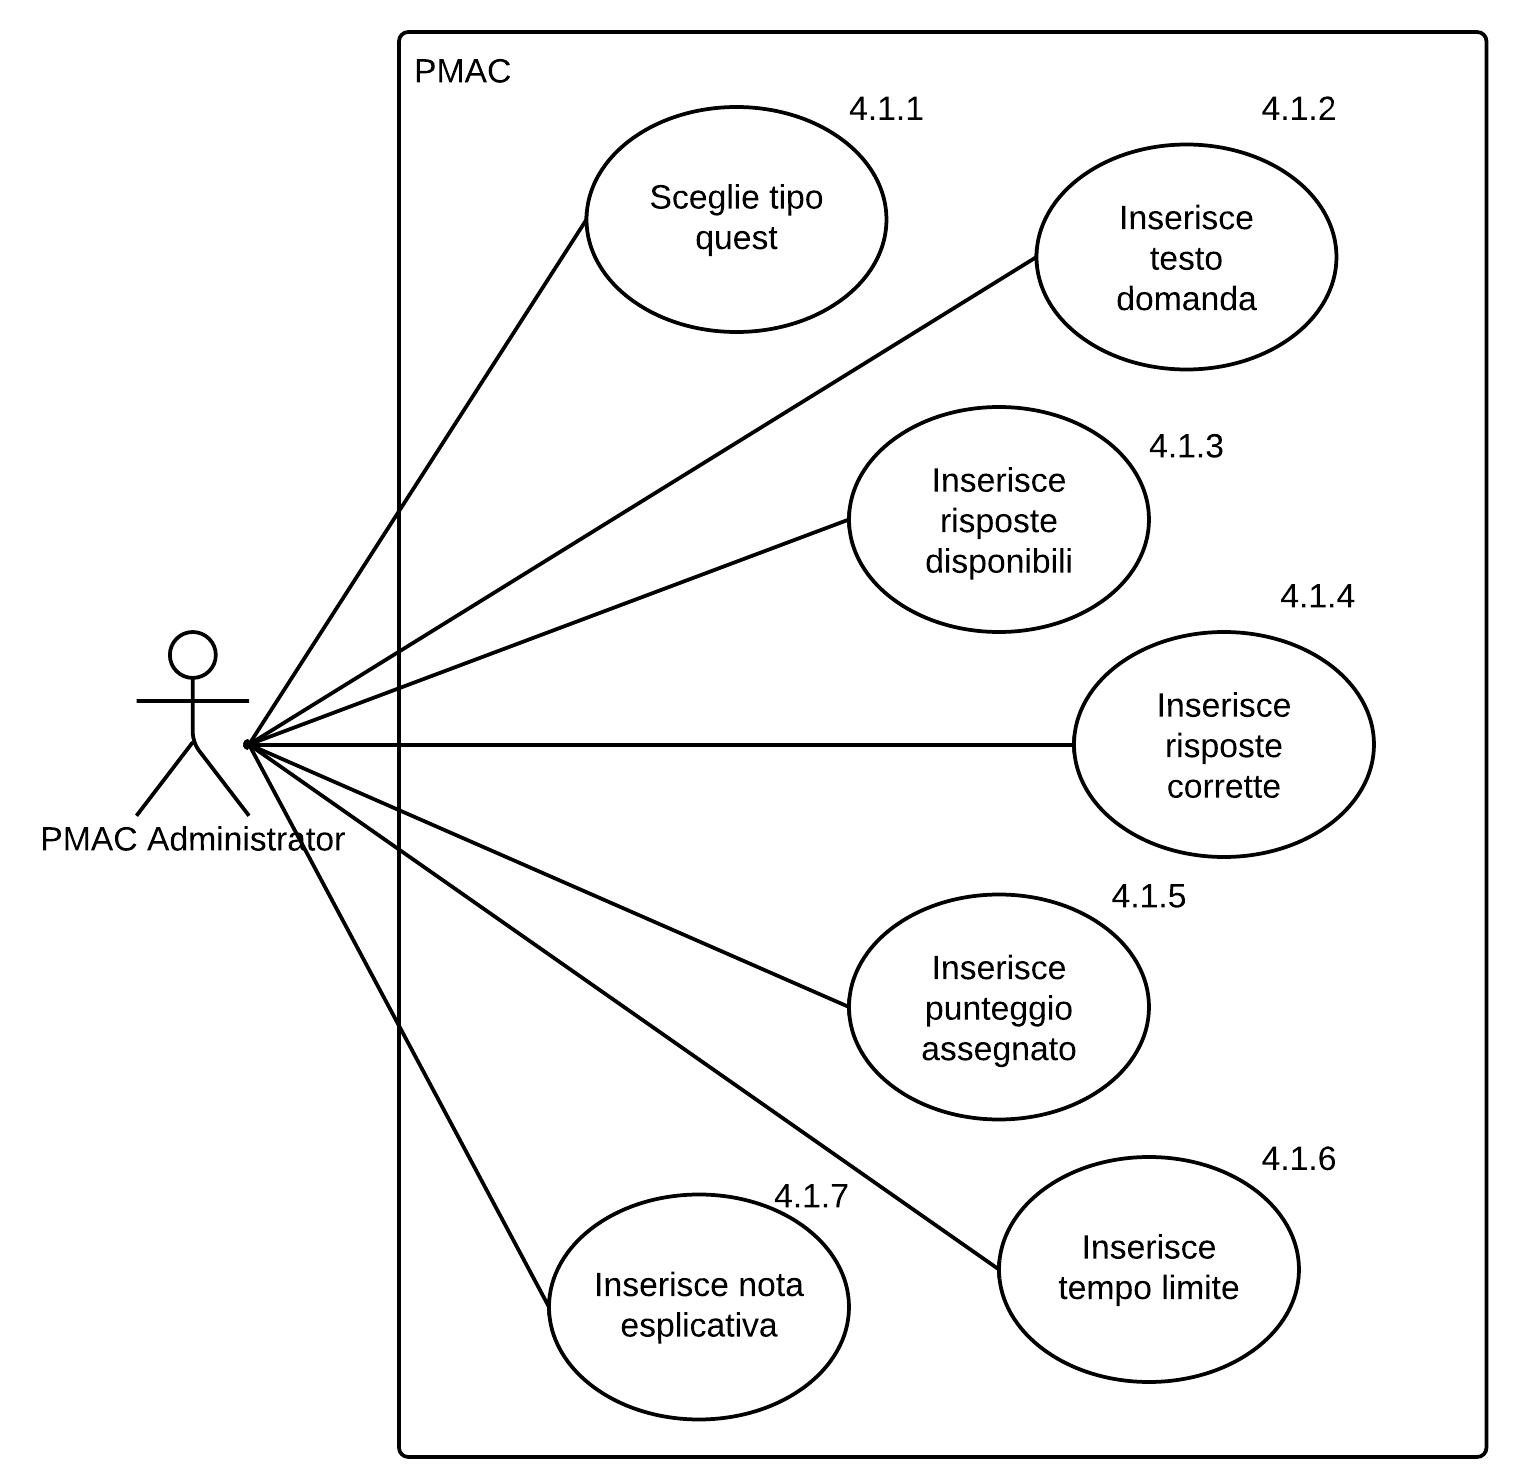
\includegraphics[scale=0.9]{images/cap1/UseCase/Uc4_1} % vedi Lateximpazienye pg67
\end{figure}

\begin{itemize}
\item \textbf{Attori coinvolti}:\\
\emph{- PMAC Administrator}: amministratore PMAC.

\item \textbf{Precondizione}:\\
L'attore che interagisce con il sistema deve possedere un account e deve aver effettuato l'accesso. Il sistema si trova nella pagina dedicata alla creazione di una quest. 

\item \textbf{Postcondizione}:\\
La nuova quest è stata creata e salvata correttamente nel sistema. Il sistema si trova nella pagina dedicata alla gestione delle quest.

\item \textbf{Scenario principale}:\\
- PMAC Administrator può scegliere il tipo della quest che sta creando tra le seguenti tipologie di quest: quest composte da solo testo, quest testuali con foto, quest testuali con video o quest con QR code. Il PMAC Administrator deve poter inserire ogni elemento che specifica le tipologie di quest. [Uc 4.1.1]\\
- PMAC Administrator può inserire il testo principale della quest che può contenere la domanda o una spiegazione del compito cognitivo da svolgere, le risposte disponibili per la quest specificando quali sono quelle corrette.[Uc 4.1.2 + Uc 4.1.3 + Uc 4.1.4]\\
- PMAC Administrator può inserire il numero di punti che saranno assegnati allo User che risponderà correttamente alla quest. [Uc 4.1.5]\\
- PMAC Administrator può inserire il tempo limite, in caso di risposta temporizzata, entro il quale lo User dovrà rispondere alla quest. [Uc 4.1.6]\\
- PMAC Administrator può inserire una nota esplicativa che potrà essere visualizzata in caso di risposta errata da parte di uno User. [Uc 4.1.7]

\item \textbf{Scenario alternativo}:\\
PMAC Administrator non conferma la creazione della nuova quest ed esce dalla pagina dedicata alla creazione di una quest. Il sistema ritorna nella pagina dedicata alla gestione delle quest.
\end{itemize}


\subsection{Uc 5: Gestisce i clienti}
% inserire una figura
\begin{figure}[ht]
\centering
\caption{Uc 5: Gestisce i clienti}
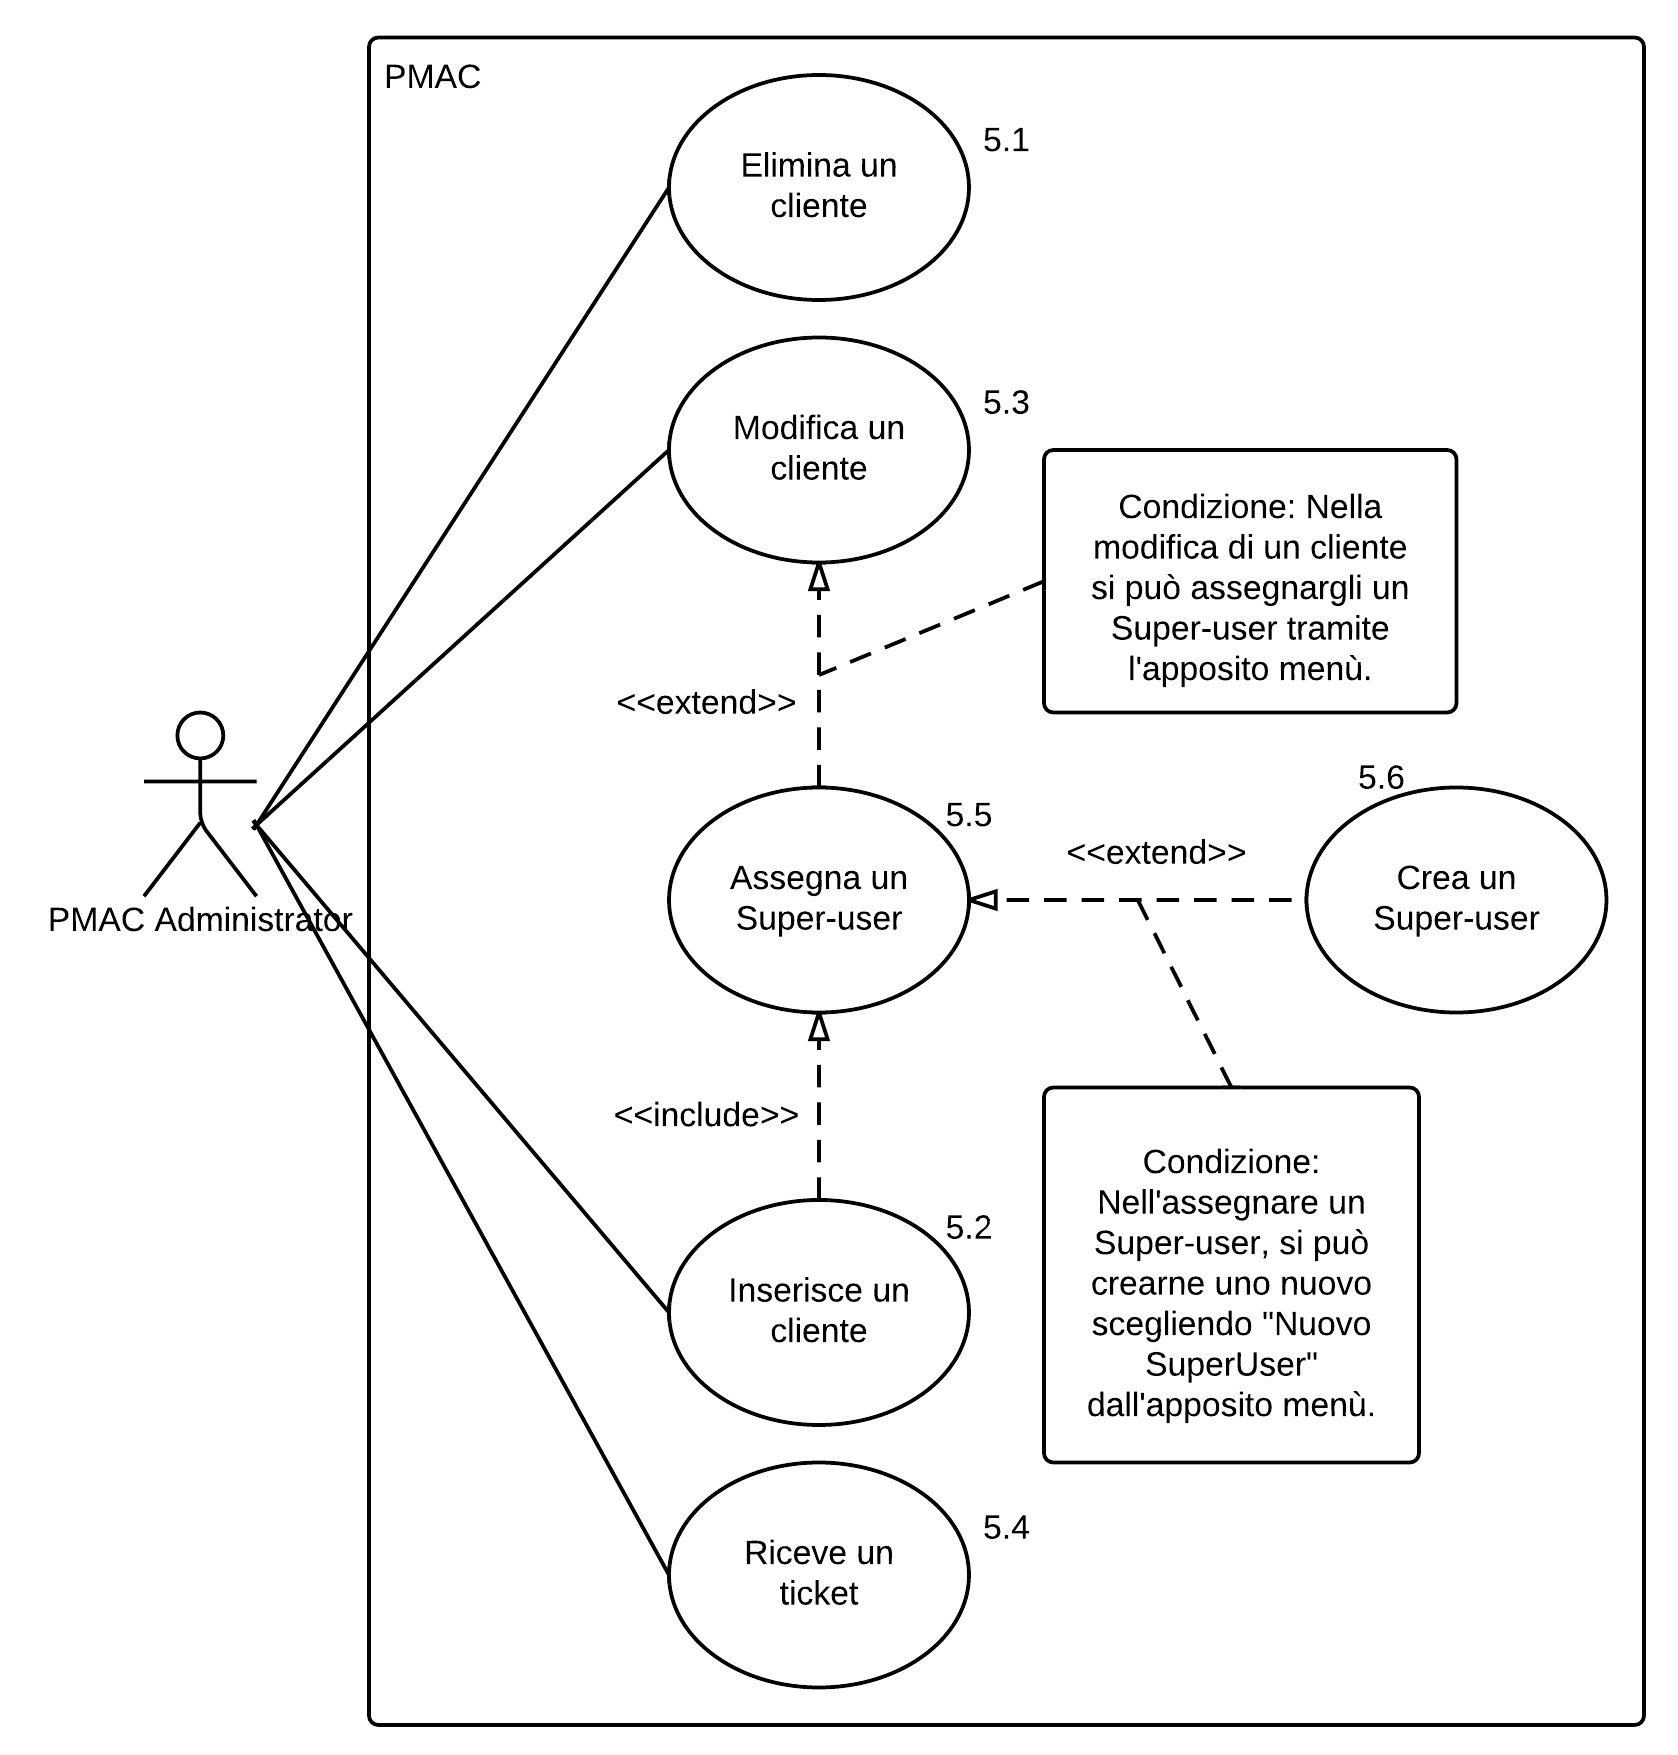
\includegraphics[scale=0.9]{images/cap1/UseCase/Uc5} % vedi Lateximpazienye pg67
\end{figure}

\begin{itemize}
\item \textbf{Attori coinvolti}:\\
PMAC Administrator: amministratore PMAC.

\item \textbf{Precondizione}:\\
PMAC Administrator deve possedere un account e deve aver effettuato l'accesso al sistema. Il sistema si trova nella pagina dedicata alla gestione degli account aziendali.

\item \textbf{Postcondizione}:\\
Le modifiche al cliente, la sua creazione o l'eliminazione sono state eseguite correttamente. Il sistema si trova nella pagina dedicata alla gestione degli account aziendali.

\item \textbf{Scenario principale}:\\
- PMAC Administrator può eliminare un cliente dal sistema. [Uc 5.1]\\
- PMAC Administrator può inserire o modificare un cliente. [Uc 5.2 + Uc 5.3]\\
- PMAC Administrator può assegnare un Super-user al cliente ed eventualmente crearne uno. [Uc 5.5 + Uc 5.6]\\
- PMAC Administrator può ricevere un ticket del sistema mandatogli da un Super-user e risolvere le problematiche descritte. [Uc 5.4]
\end{itemize}

%\newpage

\subsection{Uc 5.2: Inserisce un cliente}
% inserire una figura
\begin{figure}[ht]
\centering
\caption{Uc 5.2: Inserisce un cliente}
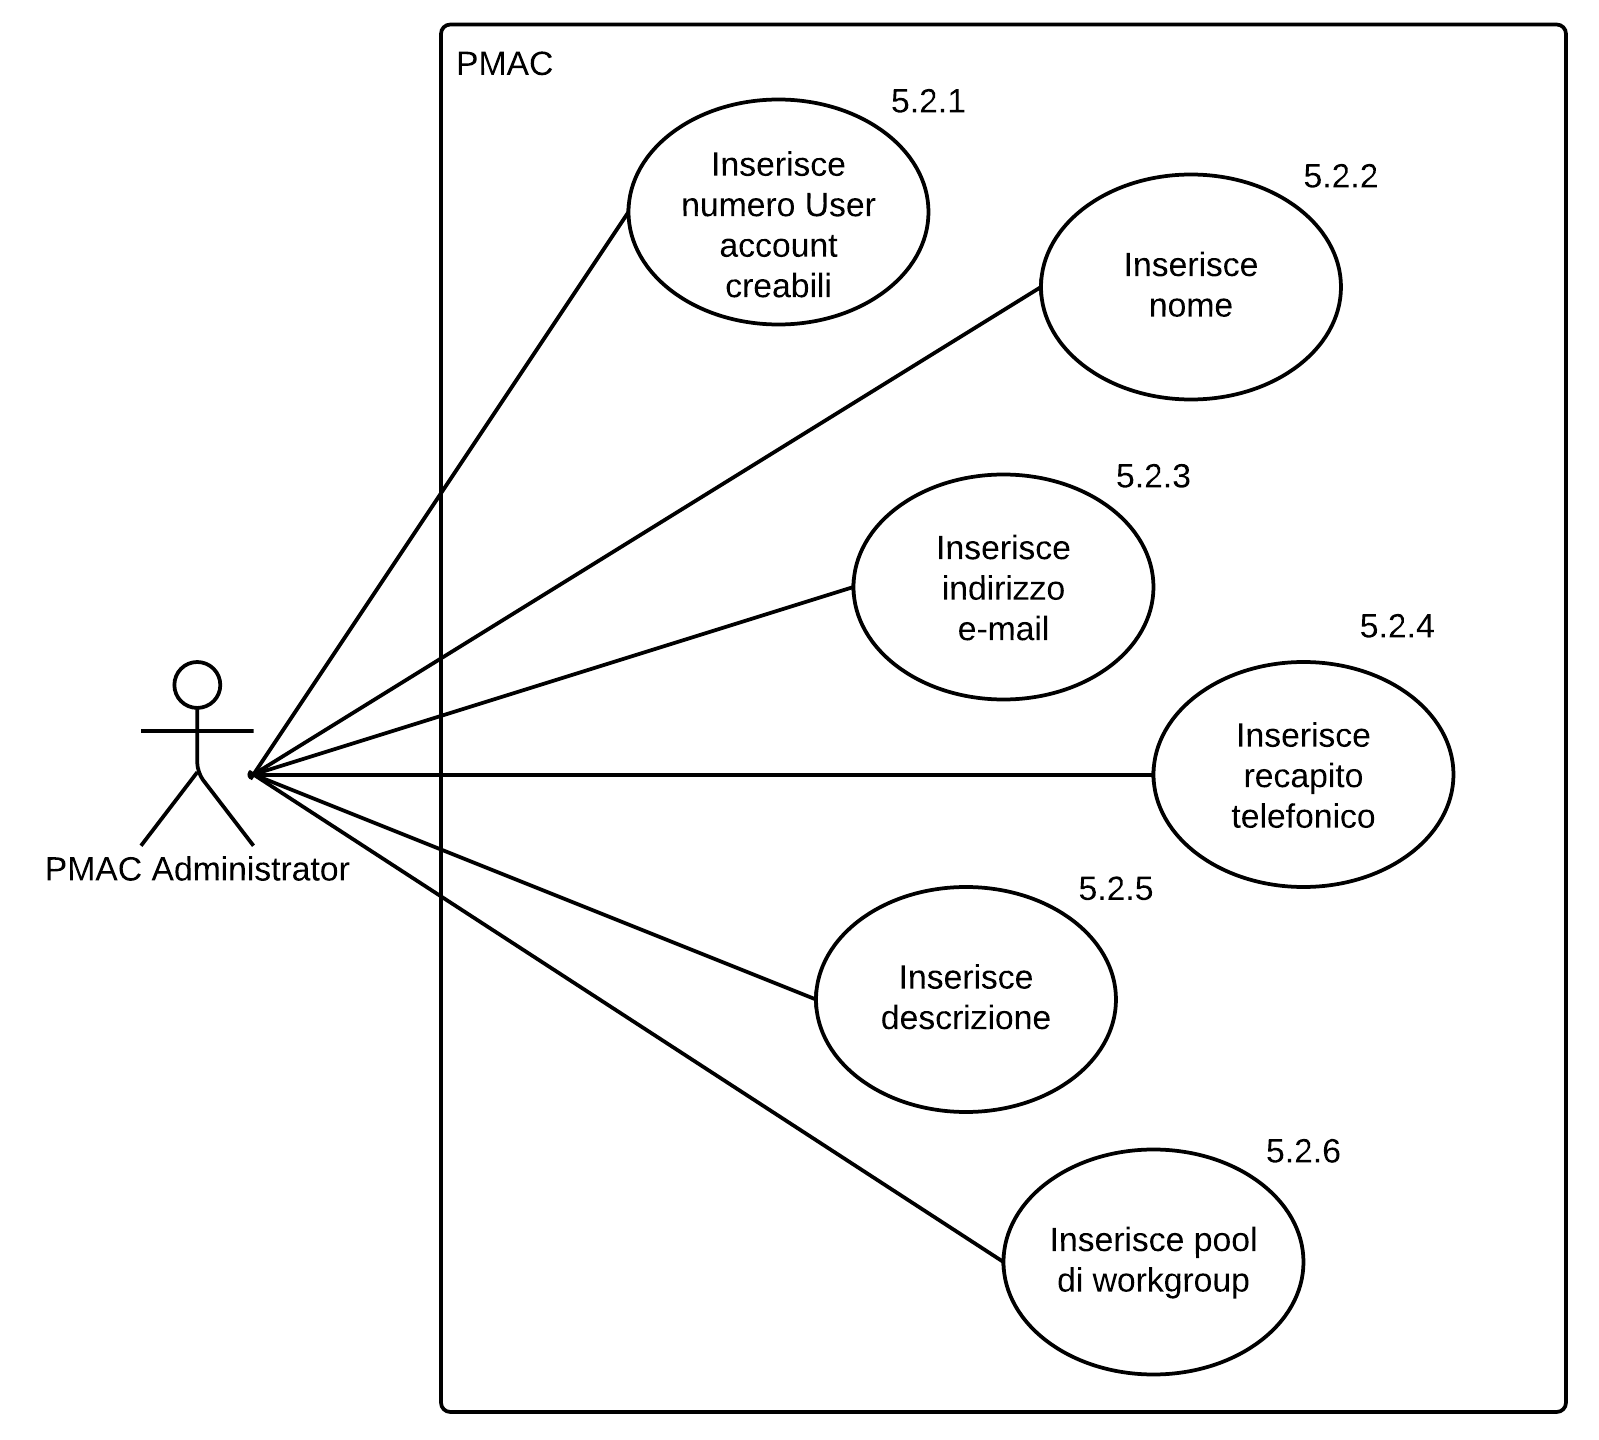
\includegraphics[scale=0.9]{images/cap1/UseCase/Uc5_2} % vedi Lateximpazienye pg67
\end{figure}

\begin{itemize}
\item \textbf{Attori coinvolti}:\\
PMAC Administrator: amministratore PMAC.

\item \textbf{Precondizione}:\\
PMAC Administrator deve possedere un account e deve aver effettuato l'accesso al sistema. Il sistema si trova nella pagina dedicata all'inserimento di un nuovo account cliente.

\item \textbf{Postcondizione}:\\
L'inserimento del cliente è stato eseguito correttamente. Il sistema si trova nella pagina dedicata alla gestione degli account aziendali.

\item \textbf{Scenario principale}:\\
- PMAC Administrator può specificare il numero totale di account creabili dal cliente a seconda della licenza acquistata. [Uc 5.2.1]\\
- PMAC Administrator può inserire il nome del cliente. [Uc 5.2.2]\\
- PMAC Administrator può inserire l'indirizzo e-mail del cliente. [Uc 5.2.3]\\
- PMAC Administrator può inserire un recapito telefonico del cliente. [Uc 5.2.4]\\
- PMAC Administrator può inserire una descrizione del cliente. [Uc 5.2.5]\\
- PMAC Administrator può specificare il pool di workgroup dedicati al cliente. [Uc 5.2.6]

\item \textbf{Scenario alternativo}:\\
PMAC Administrator non conferma l'inserimento del nuovo cliente. Il sistema ritorna alla pagina dedicata alla gestione degli account aziendali.

\end{itemize}

%\newpage

\subsection{Uc 5.3: Modifica un cliente}
% inserire una figura
\begin{figure}[ht]
\centering
\caption{Uc 5.3: Modifica un cliente}
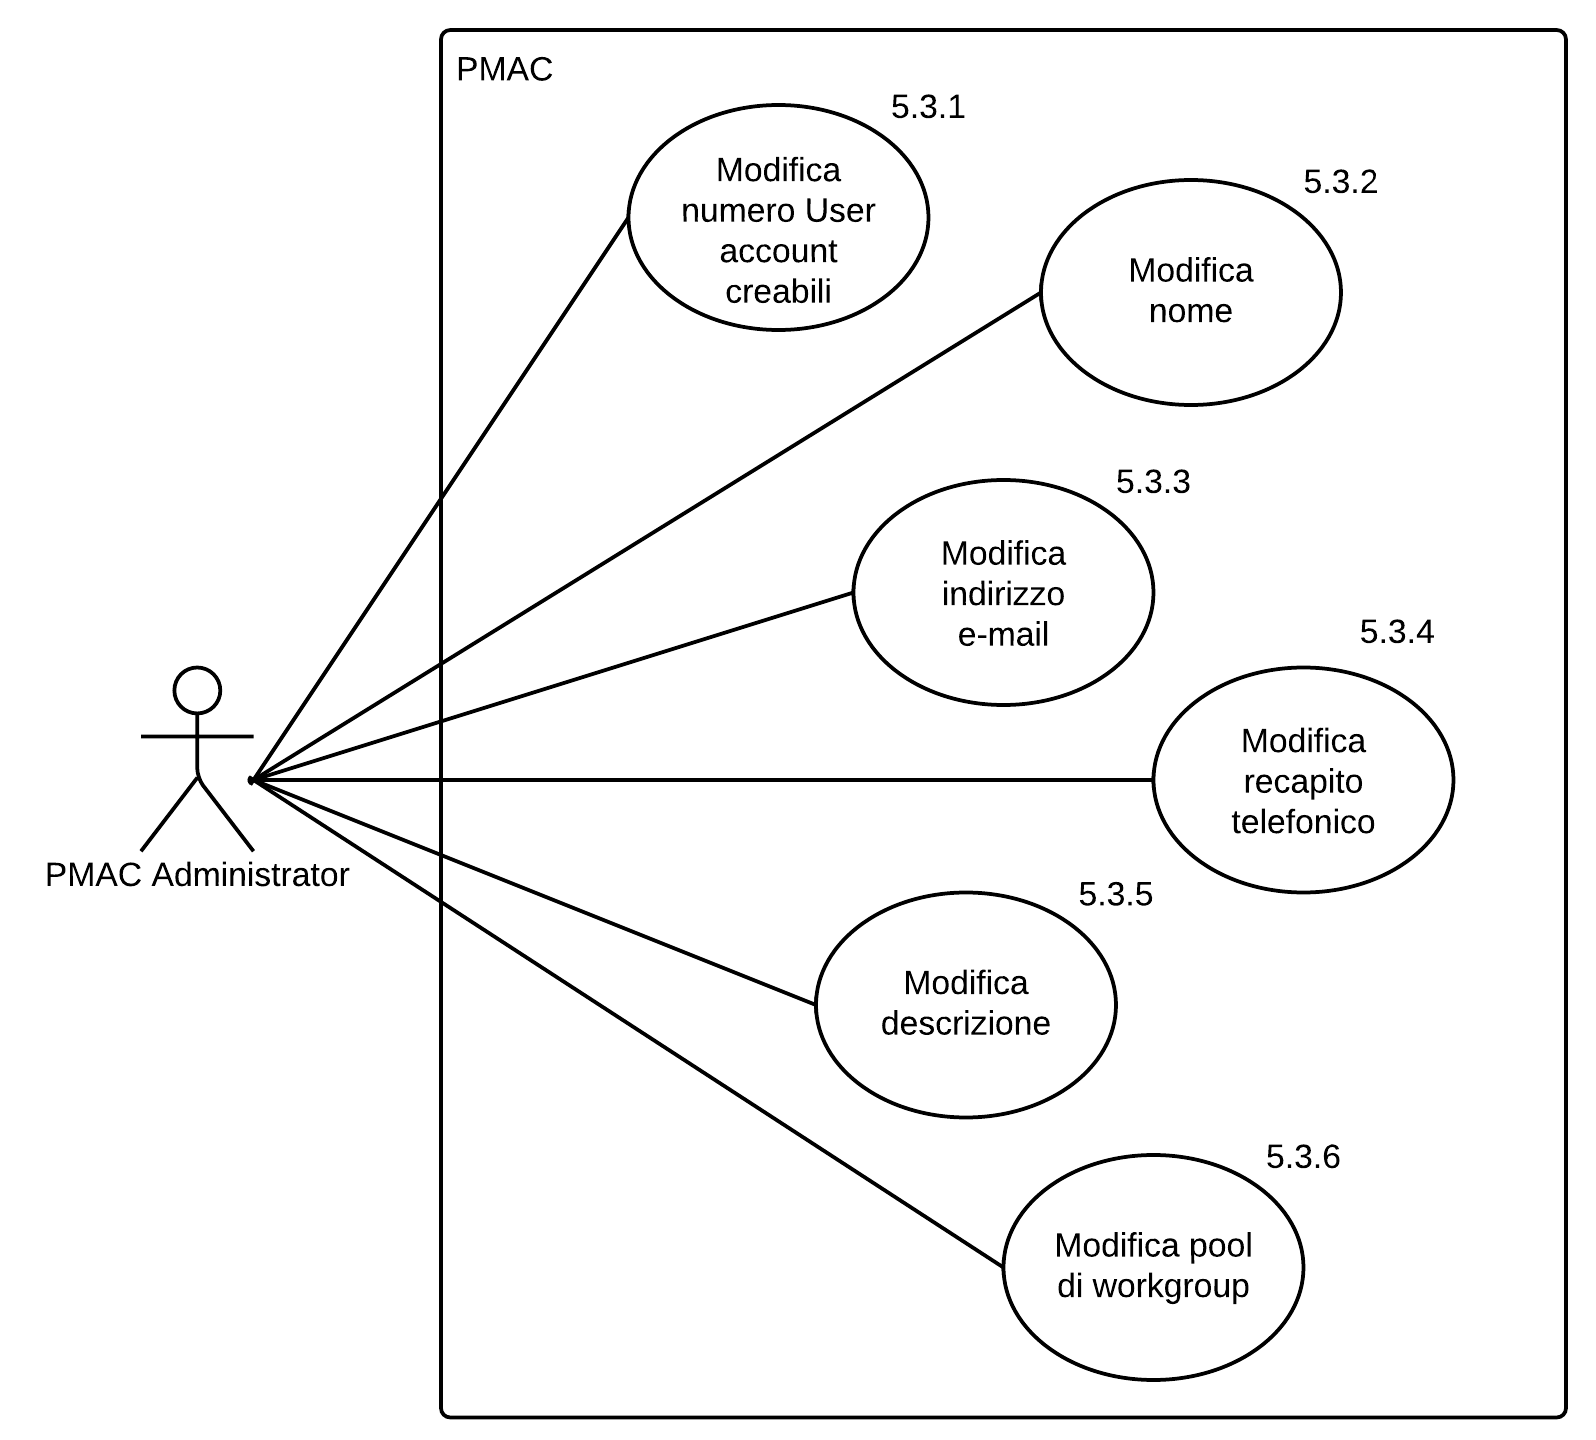
\includegraphics[scale=0.9]{images/cap1/UseCase/Uc5_3} % vedi Lateximpazienye pg67
\end{figure}

\begin{itemize}
\item \textbf{Attori coinvolti}:\\
PMAC Administrator: amministratore PMAC.

\item \textbf{Precondizione}:\\
PMAC Administrator deve possedere un account e deve aver effettuato l'accesso al sistema. Il sistema si trova nella pagina dedicata alla modifica di un account aziendale.

\item \textbf{Postcondizione}:\\
Le modifiche apportate al cliente sono state salvate correttamente. Il sistema si trova nella pagina dedicata alla gestione degli account aziendali.

\item \textbf{Scenario principale}:\\
- PMAC Administrator può modificare il numero totale di account creabili dal cliente. [Uc 5.3.1]\\
- PMAC Administrator può modificare il nome del cliente. [Uc 5.3.2]\\
- PMAC Administrator può modificare l'indirizzo e-mail del cliente. [Uc 5.3.3]\\
- PMAC Administrator può modificare un recapito telefonico del cliente. [Uc 5.3.4]\\
- PMAC Administrator può modificare una descrizione del cliente. [Uc 5.3.5]\\
- PMAC Administrator può modificare, aggiungendo o eliminando più workgroup, il pool dedicato al cliente. [Uc 5.3.6]

\item \textbf{Scenario alternativo}:\\
PMAC Administrator non conferma le modifiche ai dati del cliente. Il sistema ritorna alla pagina dedicata alla gestione degli account aziendali.

\end{itemize}


\subsection{Uc 6: Interagisce con il proprio profilo}
% inserire una figura
\begin{figure}[ht]
\centering
\caption{Uc 6: Interagisce con il proprio profilo}
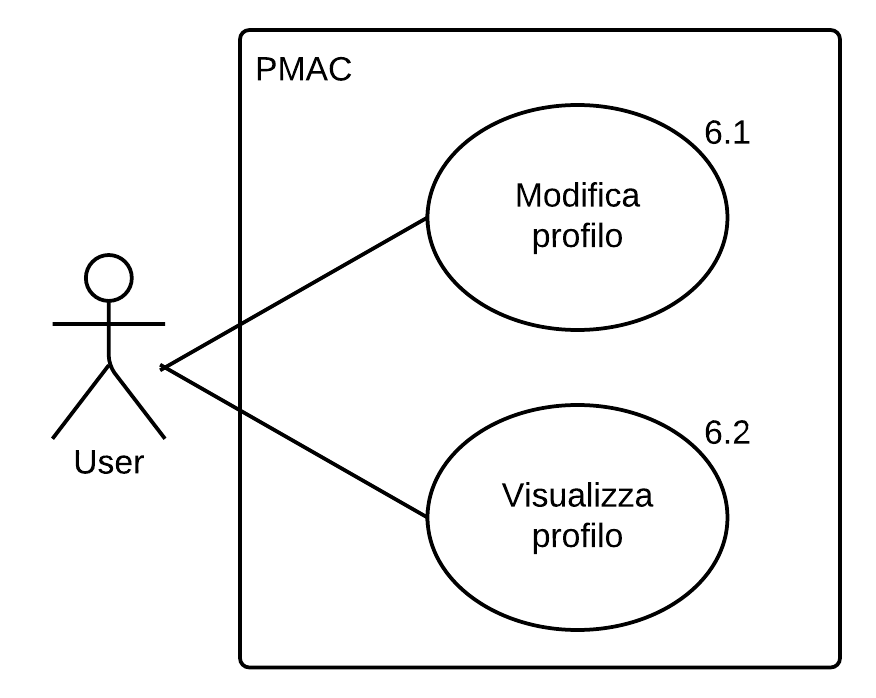
\includegraphics[scale=0.9]{images/cap1/UseCase/Uc6} % vedi Lateximpazienye pg67
\end{figure}

\begin{itemize}
\item \textbf{Attori coinvolti}:\\
- User: utente generico del sistema.

\item \textbf{Precondizione}:\\
L'utente che interagisce con il sistema deve possedere un account e deve aver effettuato l'accesso. Il sistema si trova nella pagina principale dedicata allo User.

\item \textbf{Postcondizione}:\\
Le visualizzazioni/modifiche al profilo sono state eseguite correttamente. 

\item \textbf{Scenario principale}:\\
- User può modificare il proprio profilo, portando cambiamenti ai suoi dati personali. [Uc 6.1]\\
- User può visualizzare il proprio profilo. [Uc 6.2]
\end{itemize}

\newpage

\subsection{Uc 6.1: Modifica profilo}
% inserire una figura
\begin{figure}[ht]
\centering
\caption{Uc 6.1: Modifica profilo}
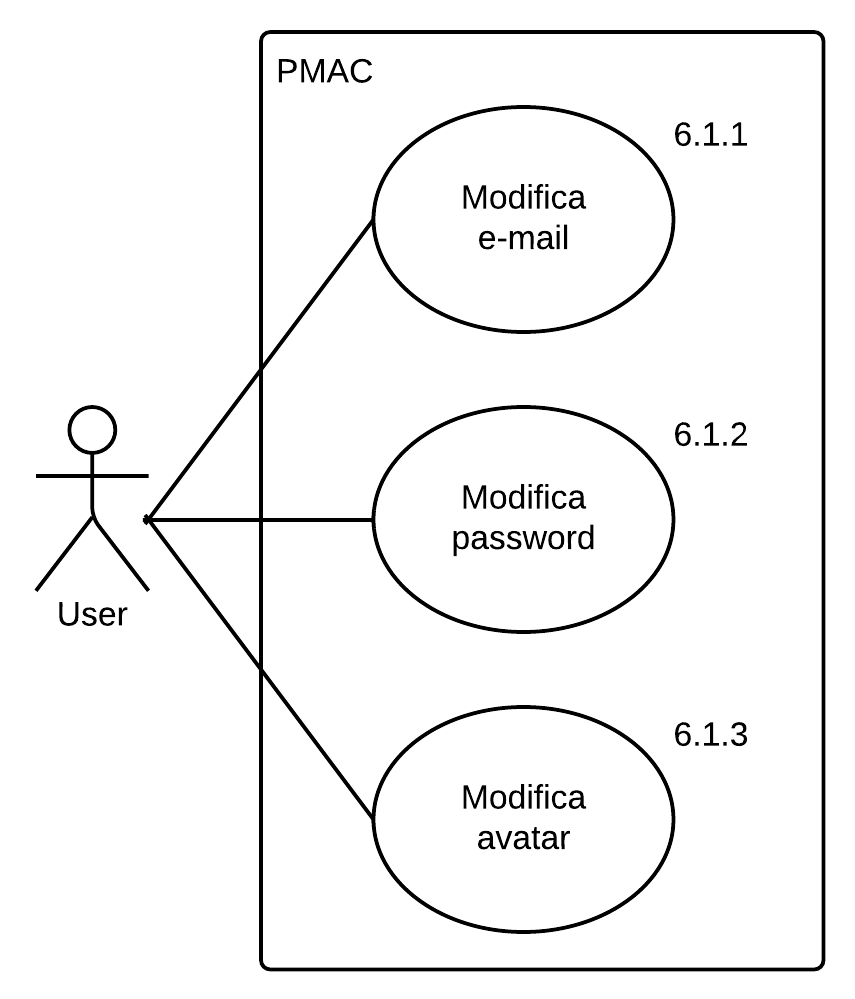
\includegraphics[scale=0.9]{images/cap1/UseCase/Uc6_1} % vedi Lateximpazienye pg67
\end{figure}

\begin{itemize}
\item \textbf{Attori coinvolti}:\\
- User: utente generico del sistema.

\item \textbf{Precondizione}:\\
L'utente che interagisce con il sistema deve possedere un account e deve aver effettuato l'accesso. Il sistema si trova nella pagina dedicata alla modifica del profilo utente.

\item \textbf{Postcondizione}:\\
Le modifiche al profilo sono state eseguite correttamente. Il sistema si trova nella pagina principale dedicata allo User.

\item \textbf{Scenario principale}:\\
- User può modificare il proprio indirizzo e-mail. [Uc 6.1.1]\\
- User può modificare la propria password. [Uc 6.1.2]\\
- User può modificare il proprio avatar. [Uc 6.1.3]

\item \textbf{Scenario alternativo}:\\
Lo User non conferma le modifiche effettuate al proprio profilo, il sistema ritorna alla pagina principale dedicata allo User mantenendo correttamente salvati i dati dello stesso.

\end{itemize}


% --------------------------------------------------------------------

% ANALISI DEI REQUISITI ( 4° CAPITOLO) 

\newpage
\comment{
\section{Analisi dei requisiti}

\thispagestyle{fancy}

\subsection{Classificazione dei requisiti}
Di seguito viene riportato l'elenco dei requisiti del sistema PMAC.
I requisiti vengono organizzati in forma gerarchica. Ogni requisito può quindi avere più sotto-requisiti.\\
Quando ognuno di questi sotto-requisiti viene soddisfatto allora il requisito di livello superiore viene soddisfatto.\\
\\
La notazione utilizzata è la seguente:\\
	
<F|P|Q|V|I><o|d|z>-X<.Y<.Z> >\\

dove le seguenti sigle indicano:
\begin{itemize}
\item[\textbf{F:}] requisito funzionale
\item[\textbf{P:}] requisito prestazionale
\item[\textbf{Q:}] requisito di qualità
\item[\textbf{V:}] requisito di vincolo
\item[\textbf{I:}] requisito di interfacciamento\\
\end{itemize}
\begin{itemize}
\item[\textbf{o:}] obbligatorio
\item[\textbf{d:}] desiderabile
\item[\textbf{z:}] opzionale\\
\end{itemize}
\begin{itemize}
\item[\textbf{X:}] requisito di primo livello
\item[\textbf{Y:}] sotto-requisito
\item[\textbf{Z:}] sotto-requisito di un sotto-requisito\\
\end{itemize}
I campi Y e Z possono essere assenti.

\newpage

\subsection{Requisiti funzionali}

\subsubsection{Requisiti funzionali obbligatori}

\begin{longtable}{|p{1,4cm}|p{10,0cm}|p{1,6cm}|}
\caption{Requisiti funzionali obbligatori}\\
\hline
\endfirsthead
\multicolumn{3}{r}{\textit{(Continua alla pagina successiva)}}
\endfoot
\multicolumn{3}{l}{\textit{(Continua dalla pagina precedente)}}
\endhead
\hline
\endlastfoot
\textbf{Codice}& \textbf{Descrizione}& \textbf{Fonte}\\
\hline
Fo-1 & Il sistema deve permettere al PMAC Administrator la creazione di workgroup che rappresentano il dipartimento di appartenenza di uno User & Interno\\
\hline
Fo-1.1 & Uno User può appartenere ad un solo workgroup & Interno\\
\hline
Fo-2 & Il sistema deve permettere al PMAC Administrator la gestione dei profili delle aziende clienti & Proponente\\
\hline
Fo-2.1 & Il sistema deve permettere al PMAC Administrator l'assegnazione/abilitazione delle metriche per la gamification alle varie aziende & Proponente\\
\hline
Fo-2.1.1 & Il sistema deve permettere la creazione di achievement che consistono in un tipo che specifica come verrà ottenuto un achievement(per tempo di risposta, punteggio, numero o percentuale di risposte corrette), un nome, una descrizione, un'immagine e un campo dati che indica a che valore viene sbloccato l'achievement & Capitolato\\
\hline
Fo-2.1.2 & Il sistema deve permettere la creazione di badge che consistono in un nome, una descrizione e un'immagine & Capitolato\\
\hline
Fo-2.2 & Il sistema deve permettere al PMAC Administrator l'aggiunta del profilo di un'azienda & Proponente\\
\hline
Fo-2.2.1 & Il sistema deve permettere l'inserimento del numero di User account creabili dall'azienda & Proponente\\
\hline
Fo-2.2.2 & Il sistema deve permettere l'inserimento del nome & Interno\\
\hline
Fo-2.2.3 & Il sistema deve permettere l'inserimento di un recapito telefonico & Interno\\
\hline
Fo-2.2.4 & Il sistema deve permettere l'inserimento di un indirizzo email & Interno\\
\hline
Fo-2.2.5 & Il sistema deve permettere l'inserimento di una descrizione dell'azienda & Interno\\
\hline
Fo-2.2.6 & Il sistema deve permettere l'assegnazione di un pool di workgroup all'azienda & Interno\\
\hline
Fo-2.2.7 & Il sistema deve permettere la creazione di un Super-User associato all'azienda che consta delle stesse informazioni di uno User & Interno\\
\hline
Fo-2.3 & Il sistema deve permettere al PMAC Administrator la modifica del profilo di un'azienda & Interno\\
\hline
Fo-2.3.1 & Il sistema deve permettere la modifica del numero di User account creabili dall'azienda & Interno\\
\hline
Fo-2.3.2 & Il sistema deve permettere la modifica del nome & Interno\\
\hline
Fo-2.3.3 & Il sistema deve permettere la modifica del recapito telefonico & Interno\\
\hline
Fo-2.3.4 & Il sistema deve permettere la modifica dell'indirizzo email & Interno\\
\hline
Fo-2.3.5 & Il sistema deve permettere la modifica della descrizione dell'azienda & Interno\\
\hline
Fo-2.3.6 & Il sistema deve permettere la modifica del pool di workgroup assegnato ad una azienda & Interno\\
\hline
Fo-2.3.7 & Il sistema deve permettere la modifica dei Super-User associati all'azienda & Interno\\
\hline
Fo-2.4 & Il sistema deve permettere al PMAC Administrator l'eliminazione del profilo di un'azienda & Interno\\
\hline
Fo-2.5 & Il sistema deve permettere al PMAC Administrator la ricezione di ticket inviati dalle aziende & Proponente\\
\hline
Fo-3 & Il sistema deve permettere al PMAC Administrator la gestione delle quest & Capitolato\\
\hline
Fo-3.1 & Il sistema deve permettere al PMAC Administrator la creazione di quest & Capitolato\\
\hline
Fo-3.1.1 & Il sistema deve permettere l'inserimento del tipo di quest che consiste in Vero/Falso, a risposta multipla, con immagini, con video o scansione QR & Capitolato\\
\hline
Fo-3.1.2 & Il sistema deve permettere l'inserimento del testo della quest & Capitolato\\
\hline
Fo-3.1.3 & Il sistema deve permettere l'inserimento delle risposte disponibili & Interno\\
\hline
Fo-3.1.4 & Il sistema deve permettere l'inserimento delle risposte corrette & Interno\\
\hline
Fo-3.1.5 & Il sistema deve permettere l'inserimento del punteggio assegnato alla risoluzione della quest & Interno\\
\hline
Fo-3.1.6 & Il sistema deve permettere l'inserimento di un tempo limite per la risoluzione della quest & Capitolato\\
\hline
Fo-3.1.7 & Il sistema deve permettere l'inserimento di una nota esplicativa da visualizzarsi nel caso di risposta errata & Interno\\
\hline
Fo-3.2 & Il sistema deve permettere al PMAC Administrator l'associazione di una quest ai diversi workgroup & Interno\\
\hline
Fo-3.3 & Il sistema deve permettere al PMAC Administrator la rimozione di quest & Interno\\
\hline
Fo-4 & Il sistema deve permettere al Super-user la gestione degli User & Proponente\\
\hline
Fo-4.1 & Il sistema deve permettere al Super-user di registrare nuovi User entro il limite imposto dal PMAC Administrator & Proponente\\
\hline
Fo-4.1.1 & Il sistema deve permettere di specificare il tipo di User (Desktop-User o un Mobile-User) & Capitolato\\
\hline
Fo-4.1.2 & Il sistema deve permettere l'inserimento del nome & Interno\\
\hline
Fo-4.1.3 & Il sistema deve permettere l'inserimento del cognome & Interno\\
\hline
Fo-4.1.4 & Il sistema deve permettere l'inserimento dell'indirizzo email & Interno\\
\hline
Fo-4.1.5 & Il sistema deve permettere l'inserimento della password & Interno\\
\hline
Fo-4.1.6 & Il sistema deve permettere l'inserimento di un avatar & Interno\\
\hline
Fo-4.1.7 & Il sistema deve permettere l'associazione dello User ad uno dei workgroup disponibili all'azienda & Proponente\\
\hline
Fo-4.2 & Il sistema deve permettere al Super-user di modificare il profilo di uno User & Interno\\
\hline
Fo-4.2.1 & Il sistema deve permettere la modifica della tipologia di User (Desktop-User o un Mobile-User) & Capitolato\\
\hline
Fo-4.2.2 & Il sistema deve permettere la modifica del nome & Interno\\
\hline
Fo-4.2.3 & Il sistema deve permettere la modifica del cognome & Interno\\
\hline
Fo-4.2.4 & Il sistema deve permettere la modifica dell'indirizzo email & Interno\\
\hline
Fo-4.2.5 & Il sistema deve permettere la modifica della password & Interno\\
\hline
Fo-4.2.6 & Il sistema deve permettere la modifica dell'avatar & Interno\\
\hline
Fo-4.2.7 & Il sistema deve permettere la modifica del workgroup associato allo User & Proponente\\
\hline
Fo-4.3 & Il sistema deve permettere al Super-user di eliminare uno User & Interno\\
\hline
Fo-4.4 & Il sistema deve permettere al Super-user la visualizzazione dei profili e delle statistiche di tutti gli User & Proponente\\
\hline
Fo-4.5 & Il Super-user deve poter svolgere tutte le attività disponibili a uno User & Proponente\\
\hline
Fo-4.6 & Il Super-user deve poter aprire ticket di richiesta/assistenza destinati al PMAC Administrator che consistono di un titolo, una data e una descrizione del problema riscontrato & Proponente\\
\hline
Fo-5 & Gli Desktop-User potranno risolvere tutte le tipologie di quest, escluse le quest che richiedono la scansione di codici QR & Capitolato\\
\hline
Fo-5.1 & I Desktop-User possono eseguire quest testuali che si dividono in domande vero/falso, risposta chiusa tra un certo numero alternative e risposta multipla & Capitolato\\
\hline
Fo-5.2 & I Desktop-User possono eseguire quest con immagini & Capitolato\\
\hline
Fo-5.3 & I Desktop-User possono eseguire quest con video & Capitolato\\
\hline
Fo-6 & I Mobile-User potranno risolvere tutte le tipologie di quest & Capitolato\\
\hline
Fo-6.1 & I Mobile-User possono eseguire quest testuali che si dividono in domande vero/falso, risposta chiusa tra un certo numero alternative e risposta multipla & Capitolato\\
\hline
Fo-6.2 & I Mobile-User possono eseguire quest con immagini & Capitolato\\
\hline
Fo-6.3 & I Mobile-User possono eseguire quest con video & Capitolato\\
\hline
Fo-6.4 & I Mobile-User possono eseguire quest che richiedono la  scansione di QR-Code & Capitolato\\
\hline
Fo-7 & Il sistema deve permettere l'autenticazione degli User tramite email e password & Interno\\
\hline
Fo-8 & Il sistema deve notificare allo User la presenza di quest assegnategli & Capitolato\\
\hline
Fo-8.1 & Il sistema deve permettere allo User la visualizzazione e la risoluzione delle quest notificate & Capitolato\\
\hline
Fo-8.2 & Lo User può rifiutare di sottoporsi alle quest in seguito alla ricezione delle notifiche & Capitolato\\
\hline
Fo-8.3 & Lo User può disattivare la ricezione delle notifiche per un dato intervallo di tempo & Capitolato\\
\hline
Fo-8.4 & Lo User può richiedere quest aggiuntive & Capitolato\\
\hline
Fo-9 & Il sistema deve permettere allo User la visualizzazione delle classifiche stilate sulla base delle statistiche degli User & Capitolato\\
\hline
Fo-10 & Il sistema deve permettere allo User la gestione del proprio profilo & Interno\\
\hline
Fo-10.1 & Il sistema deve permettere allo User la modifica del proprio profilo & Interno\\
\hline
Fo-10.1.1 & Il sistema deve permettere la modifica dell'indirizzo email & Interno\\
\hline
Fo-10.1.2 & Il sistema deve permettere la modifica della password & Interno\\
\hline
Fo-10.1.3 & Il sistema deve permettere la modifica dell'avatar & Interno\\
\hline
Fo-10.2 & Il sistema deve permettere allo User la visualizzazione del proprio profilo & Interno\\
\hline
Fo-10.3 & Il sistema deve permettere allo User la visualizzazione delle statistiche personali & Interno\\
\hline
Fo-10.3.1 & Il sistema deve permettere la visualizzazione del punteggio totale & Interno\\
\hline
Fo-10.3.2 & Il sistema deve permettere la visualizzazione del numero totale di quest effettuate & Interno\\
\hline
Fo-10.3.3 & Il sistema deve permettere la visualizzazione del numero totale di risposte corrette date & Interno\\
\hline
Fo-10.3.4 & Il sistema deve permettere la visualizzazione della percentuale di risposte corrette date a fronte dei tentativi di risoluzione effettuati & Interno\\
\hline
Fo-10.3.5 & Il sistema deve permettere la visualizzazione del tempo medio di risposta & Interno\\
\hline
Fo-10.4 & Il sistema deve permettere allo User la visualizzazione dei badge e degli achievement ottenuti & Interno\\
%\hline

\end{longtable}

\newpage

\subsection{Requisiti funzionali desiderabili}
\begin{longtable}{|p{1,4cm}|p{10,0cm}|p{1,6cm}|}
\caption{Requisiti funzionali desiderabili}\\
\hline
\endfirsthead
\multicolumn{3}{r}{\textit{(Continua alla pagina successiva)}}
\endfoot
\multicolumn{3}{l}{\textit{(Continua dalla pagina precedente)}}
\endhead
\hline
\endlastfoot
\textbf{Codice}& \textbf{Descrizione}& \textbf{Fonte}\\
\hline
Fd-1 & Il sistema deve permettere allo User la visualizzazione dei profili degli altri User & Proponente\\
\hline
Fd-2 & Il sistema, al completamento di una quest, deve permettere allo user la visualizzazione della soluzione o di una breve nota esplicativa & Proponente\\
\end{longtable}

\subsubsection{Requisiti funzionali opzionali}
\begin{longtable}{|p{1,4cm}|p{10,0cm}|p{1,6cm}|}
\caption{Requisiti funzionali opzionali}\\
\hline
\endfirsthead
\multicolumn{3}{r}{\textit{(Continua alla pagina successiva)}}
\endfoot
\multicolumn{3}{l}{\textit{(Continua dalla pagina precedente)}}
\endhead
\hline
\endlastfoot
\textbf{Codice}& \textbf{Descrizione}& \textbf{Fonte}\\
\hline
Fz-1 & Il sistema deve prevedere una tipologia di quest risolvibile da postazione fissa con l'ausilio di un dispositivo mobile che consiste nella scansione di un Qr-Code & Capitolato\\
\hline
Fz-2 & Le funzionalità del sistema sono studiate per invogliare l'utente alla partecipazione & Proponente\\
\hline
Fz-2.1 & Gli User possono formare delle squadre con altri User, le quali avranno un nome e un punteggio proprio derivato dal successo dei componenti del gruppo all'interno del sistema & Interno\\
\hline
Fz-2.2 & Agli User verrà associato un grado all'interno della propria squadra che muterà secondo l'apporto di punti alla squadra & Interno\\
\hline
Fz-2.3 & Ad ogni User è assegnato un livello che aumenta con il conseguimento di successi all'interno del "gioco" & Interno\\
\hline
Fz-2.4 & Gli User possono spedire messaggi testuali ad altri User & Interno\\
\hline
Fz-2.4.1 & Gli User possono spedire messaggi pubblici ad altri User che verranno visualizzati sul profilo dello User destinatario & Interno\\
\hline
Fz-2.4.2 & Gli User possono spedire messaggi privati ad altri User che verranno visualizzati solo dallo User destinatario & Interno\\
\hline
Fz-2.5 & Gli User possono visualizzare le azioni recenti compiute da altri User o squadre all'interno del sistema & Interno\\
\hline
Fz-2.5.1 & Gli User possono un feedback di apprezzamento su un'azione compiuta da altri User & Interno\\
\hline
Fz-2.5.2 & Gli User possono lasciare un commento testuale su di una delle azioni visualizzate & Interno\\
\hline
Fz-2.5.3 & I Super-user possono moderare i commenti degli User & Interno\\
\hline
Fz-3 & Il sistema deve prevedere un'interfaccia verso sensori di macchinari o altre strumentazioni & Capitolato\\

\end{longtable}

\newpage

\subsection{Requisiti di qualità}

\subsubsection{Requisiti di qualità obbligatori}

\begin{longtable}{|p{1,4cm}|p{10,0cm}|p{1,6cm}|}
\caption{Requisiti di qualità obbligatori}\\
\hline
\endfirsthead
\multicolumn{3}{r}{\textit{(Continua alla pagina successiva)}}
\endfoot
\multicolumn{3}{l}{\textit{(Continua dalla pagina precedente)}}
\endhead
\hline
\endlastfoot
\textbf{Codice}& \textbf{Descrizione}& \textbf{Fonte}\\
\hline
Qo-1 & Il sistema deve essere multiutente & Capitolato\\
\hline
Qo-2 & Il sistema deve essere robusto impedendo la perdita o corruzione dei dati dell'utente o di utilizzo del software nell'eventualità di problemi di rete & Interno\\
\hline
Qo-3 & Il sistema deve essere accompagnato dalla documentazione sui test eseguiti & Interno\\
\end{longtable}



\subsubsection{Requisiti di qualità desiderabili}

\begin{longtable}{|p{1,4cm}|p{10,0cm}|p{1,6cm}|}
\caption{Requisiti di qualità desiderabili}\\
\hline
\endfirsthead
\multicolumn{3}{r}{\textit{(Continua alla pagina successiva)}}
\endfoot
\multicolumn{3}{l}{\textit{(Continua dalla pagina precedente)}}
\endhead
\hline
\endlastfoot
\textbf{Codice}& \textbf{Descrizione}& \textbf{Fonte}\\

\hline
Qd-1 & Il sistema deve prevedere un pacchetto di installazione che installa e configura il suddetto e tutti i software da esso richiesti & Proponente\\
\hline
Qd-2 & La gestione tecnica deve essere minima e totalmente a carico del PMAC Administrator & Interno\\
\end{longtable}



\subsubsection{Requisiti di qualità opzionali}

\begin{longtable}{|p{1,4cm}|p{10,0cm}|p{1,6cm}|}
\caption{Requisiti di qualità opzionali}\\
\hline
\endfirsthead
\multicolumn{3}{r}{\textit{(Continua alla pagina successiva)}}
\endfoot
\multicolumn{3}{l}{\textit{(Continua dalla pagina precedente)}}
\endhead
\hline
\endlastfoot
\textbf{Codice}& \textbf{Descrizione}& \textbf{Fonte}\\
\hline
Qz-1 & Il sistema deve fornire un help contestuale & Interno\\
\hline
Qz-2 & Si prevede la realizzazione di un manuale di sviluppo destinato a coloro vorranno estendere il sistema & Interno\\
\end{longtable}
\vspace{0.7cm}
\newpage


\subsection{Requisiti di vincolo}
\subsubsection{Requisiti di vincolo obbligatori}

\begin{longtable}{|p{1,4cm}|p{10,0cm}|p{1,6cm}|}
\caption{Requisiti di vincolo obbligatori}\\
\hline
\endfirsthead
\multicolumn{3}{r}{\textit{(Continua alla pagina successiva)}}
\endfoot
\multicolumn{3}{l}{\textit{(Continua dalla pagina precedente)}}
\endhead
\hline
\endlastfoot
\textbf{Codice}& \textbf{Descrizione}& \textbf{Fonte}\\
\hline
Vo-1 & Il sistema deve essere permanentemente connesso ad internet & Capitolato\\
\hline
Vo-2 & Le notifiche del sistema non devono essere invasive per non interferire con il normale svolgimento delle attività lavorative & Interno\\
\end{longtable}
\vspace{0.7cm}



\subsection{Requisiti di interfacciamento}

\subsubsection{Requisiti di interfacciamento obbligatori}

\begin{longtable}{|p{1,4cm}|p{10,0cm}|p{1,6cm}|}
\caption{Requisiti di interfacciamento obbligatori}\\
\hline
\endfirsthead
\multicolumn{3}{r}{\textit{(Continua alla pagina successiva)}}
\endfoot
\multicolumn{3}{l}{\textit{(Continua dalla pagina precedente)}}
\endhead
\hline
\endlastfoot
\textbf{Codice}& \textbf{Descrizione}& \textbf{Fonte}\\
\hline
Io-1 & Il sistema deve prevedere un'interfaccia destinata al PMAC Administrator & Capitolato\\
\hline
Io-2 & Il sistema deve prevedere un'interfaccia per l'amministrazione destinata a un Super-user & Capitolato\\
\hline
Io-3 & Il sistema deve prevedere un'interfaccia User per postazione fissa & Capitolato\\
\hline
Io-4 & Il sistema deve prevedere un'interfaccia User per piattaforma mobile & Capitolato\\
\hline
Io-5 & Il sistema deve prevedere una visualizzazione a video delle notifiche ricevute anche a browser chiuso & Capitolato\\
\end{longtable}
% --------------------------------------------------------------------

% TRACCIAMENTO ( 5° CAPITOLO) 

\newpage

\section{Tracciamento}

\thispagestyle{fancy}

Di seguito sono riportate le tabelle di tracciamento tra Use Case - requisito e viceversa.\\
Requisiti di vincolo, qualitativi o di interfacciamento non sono stati tracciati da alcun Use Case in quanto non sono rappresentabili da nessuno di essi, ma derivano dalle richieste del capitolato o del proponente o da decisioni interne al gruppo in seguito allo studio del caso.\\

\subsection{Tracciamento Use Case - Requisiti}

\begin{longtable}{|p{3.5cm}|p{6.5cm}|p{3cm}|}
\caption{Tracciamento Use Case - Requisiti}\\
\hline
\endfirsthead
\multicolumn{3}{r}{\textit{(Continua alla pagina successiva)}}
\endfoot
\multicolumn{3}{l}{\textit{(Continua dalla pagina precedente)}}
\endhead
\hline
\endlastfoot
\textbf{Codice Use Case}& \textbf{Nome Use Case}& \textbf{Requisito}\\
\hline
Uc 1 & Interagisce con una quest & Fo-5 \newline Fo-6\\
\hline
\ \ \ \ Uc 1.1 & Riceve quest & Fo-8 \newline\\
\hline
\ \ \ \ Uc 1.2 & Affronta quest & Fo-8.1 \newline Fo-5 \newline Fo-5.1 \newline Fo-5.2 \newline Fo-5.3 \newline Fo-6 \newline Fo-6.1 \newline Fo-6.2 \newline Fo-6.3 \newline Fo-6.4\\
\hline
\ \ \ \ Uc 1.3 & Rifiuta quest & Fo-8.2 \newline Fo-8.3 \\
\hline
\ \ \ \ Uc 1.4 & Chiede una quest & Fo-8.4\\
\hline
Uc 2 & Visualizza statistiche & Fo-10.3\\
\hline
\ \ \ \ Uc 2.1 & Richiede le proprie statistiche & Fo-10.3.1 \newline Fo-10.3.2 \newline Fo-10.3.3 \newline Fo-10.3.4 \newline Fo-10.3.5 \newline Fo-10.4\\
\hline
\ \ \ \ Uc 2.2 & Richiede statistiche di qualsiasi User & Fo-4.4\\
\hline
Uc 3 & Gestisce utenti presso un cliente & Fo-4\\
\hline
\ \ \ \ Uc 3.1 & Crea nuovo account user & Fo-4.1 \newline Fo-4.1.2 \newline Fo-4.1.3 \newline Fo-4.1.4 \newline Fo-4.1.5 \newline Fo-4.1.6 \newline Fo-4.1.7\\
\hline
\ \ \ \ Uc 3.2 & Sceglie tipo user & Fo-4.1.1 \newline Fo-4.2.1\\
\hline
\ \ \ \ Uc 3.3 & Modifica user & Fo-4.2 \newline Fo-4.2.2 \newline Fo-4.2.3 \newline Fo-4.2.4 \newline Fo-4.2.5 \newline Fo-4.2.6 \newline Fo-4.2.7\\
\hline
\ \ \ \ Uc 3.4 & Cancella user & Fo-4.3\\
\hline
\ \ \ \ Uc 3.5 & Crea ticket & Fo-4.6\\
\hline
Uc 4 & Gestisce le quest & Fo-3\\
\hline
\ \ \ \ Uc 4.1 & Crea una quest & Fo-3.1 \newline Fo-3.1.2 \newline Fo-3.1.3 \newline Fo-3.1.4 \newline Fo-3.1.5 \newline Fo-3.1.6 \newline Fo-3.1.7\\
\hline
\ \ \ \ Uc 4.2 & Rimuove quest & Fo-3.3\\
\hline
\ \ \ \ Uc 4.3 & Assegna quest a workgroup & Fo-3.2\\
\hline
Uc 5 & Gestisce i clienti & Fo-2\\
\hline
\ \ \ \ Uc 5.1 & Elimina un cliente & Fo-2.4\\
\hline
\ \ \ \ Uc 5.2 & Inserisce un cliente & Fo-2.2 \newline Fo-2.2.1 \newline Fo-2.2.2 \newline Fo-2.2.3 \newline Fo-2.2.4 \newline Fo-2.2.5 \newline Fo-2.2.6\\
\hline
\ \ \ \ Uc 5.3 & Modifica un cliente & Fo-2.3 \newline Fo-2.3.1 \newline Fo-2.3.2 \newline Fo-2.3.3 \newline Fo-2.3.4 \newline Fo-2.3.5 \newline Fo-2.3.6 \\
\hline
\ \ \ \ Uc 5.4 & Riceve un ticket & Fo-2.5\\
\hline
\ \ \ \ Uc 5.5 & Assegna un super-user & Fo-2.2.7 \newline Fo-2.3.7\\
\hline
\ \ \ \ Uc 5.6 & Crea nuovo super-user & Fo-2.2.7 \\
\hline
Uc 6 & Interagisce con il proprio profilo & Fo-10\\
\hline
\ \ \ \ Uc 6.1 & Modifica profilo & Fo-10.1 \newline Fo-10.1.1 \newline Fo-10.1.2 \newline Fo-10.1.3\\
\hline
\ \ \ \ Uc 6.2 & Visualizza profilo & Fo-10.2\\
\hline
Uc 7 & Crea badges e achievements & Fo-2.1 \newline Fo-2.1.1 \newline Fo-2.1.2\\
\hline
Uc 8 & Visualizza classifiche & Fo-9\\
\hline
Uc 9 & Crea workgroup & Fo-1\\

\end{longtable}

\newpage

\subsection{Tracciamento Requisito - Use Case}

\begin{longtable}{|p{5cm}|p{5cm}|}
\caption{Tracciamento Requisito - Use Case}\\
\hline
\endfirsthead
\multicolumn{2}{r}{\textit{(Continua alla pagina successiva)}}
\endfoot
\multicolumn{2}{l}{\textit{(Continua dalla pagina precedente)}}
\endhead
\hline
\endlastfoot
\textbf{Codice Requisito}& \textbf{Codice Use Case}\\
\hline
Fo-1 & Uc 9\\
\hline
Fo-2 & Uc 5\\
\hline
\ \ \ \ Fo-2.1 & Uc 7\\
\hline
\ \ \ \ \ \ \ \ Fo-2.1.1 & Uc 7\\
\hline
\ \ \ \ \ \ \ \ Fo-2.1.2 & Uc 7\\
\hline
\ \ \ \ Fo-2.2 & Uc 5.2\\
\hline
\ \ \ \ \ \ \ \ Fo-2.2.1 & Uc 5.2.1\\
\hline
\ \ \ \ \ \ \ \ Fo-2.2.2 & Uc 5.2.2\\
\hline
\ \ \ \ \ \ \ \ Fo-2.2.3 & Uc 5.2.3\\
\hline
\ \ \ \ \ \ \ \ Fo-2.2.4 & Uc 5.2.4\\
\hline
\ \ \ \ \ \ \ \ Fo-2.2.5 & Uc 5.2.5\\
\hline
\ \ \ \ \ \ \ \ Fo-2.2.6 & Uc 5.2.6\\
\hline
\ \ \ \ \ \ \ \ Fo-2.2.7 & Uc 5.5 \newline Uc 5.6\\
\hline
\ \ \ \ Fo-2.3 & Uc 5.3\\
\hline
\ \ \ \ \ \ \ \ Fo-2.3.1 & Uc 5.3.1\\
\hline
\ \ \ \ \ \ \ \ Fo-2.3.2 & Uc 5.3.2\\
\hline
\ \ \ \ \ \ \ \ Fo-2.3.3 & Uc 5.3.3\\
\hline
\ \ \ \ \ \ \ \ Fo-2.3.4 & Uc 5.3.4\\
\hline
\ \ \ \ \ \ \ \ Fo-2.3.5 & Uc 5.3.5\\
\hline
\ \ \ \ \ \ \ \ Fo-2.3.6 & Uc 5.3.6\\
\hline
\ \ \ \ \ \ \ \ Fo-2.3.7 & Uc 5.5 \newline Uc 5.6\\
\hline
\ \ \ \ Fo-2.4 & Uc 5.1\\
\hline
\ \ \ \ Fo-2.5 & Uc 5.4\\
\hline
Fo-3 & Uc 4\\
\hline
\ \ \ \ Fo-3.1 & Uc 4.1\\
\hline
\ \ \ \ \ \ \ \ Fo-3.1.1 & Uc 4.1.1\\
\hline
\ \ \ \ \ \ \ \ Fo-3.1.2 & Uc 4.1.2\\
\hline
\ \ \ \ \ \ \ \ Fo-3.1.3 & Uc 4.1.3\\
\hline
\ \ \ \ \ \ \ \ Fo-3.1.4 & Uc 4.1.4\\
\hline
\ \ \ \ \ \ \ \ Fo-3.1.5 & Uc 4.1.5\\
\hline
\ \ \ \ \ \ \ \ Fo-3.1.6 & Uc 4.1.6\\
\hline
\ \ \ \ \ \ \ \ Fo-3.1.7 & Uc 4.1.7\\
\hline
\ \ \ \ Fo-3.2 & Uc 4.3\\
\hline
\ \ \ \ Fo-3.3 & Uc 4.2\\
\hline
Fo-4 & Uc 3\\
\hline
\ \ \ \ Fo-4.1 & Uc 3.1\\
\hline
\ \ \ \ \ \ \ \ Fo-4.1.1 & Uc 3.2\\
\hline
\ \ \ \ \ \ \ \ Fo-4.1.2 & Uc 3.1.1\\
\hline
\ \ \ \ \ \ \ \ Fo-4.1.3 & Uc 3.1.2\\
\hline
\ \ \ \ \ \ \ \ Fo-4.1.4 & Uc 3.1.3\\
\hline
\ \ \ \ \ \ \ \ Fo-4.1.5 & Uc 3.1.4\\
\hline
\ \ \ \ \ \ \ \ Fo-4.1.6 & Uc 3.1.6\\
\hline
\ \ \ \ \ \ \ \ Fo-4.1.7 & Uc 3.1.5\\
\hline
\ \ \ \ Fo-4.2 & Uc 3.3\\
\hline
\ \ \ \ \ \ \ \ Fo-4.2.1 & Uc 3.2\\
\hline
\ \ \ \ \ \ \ \ Fo-4.2.2 & Uc 3.3.1\\
\hline
\ \ \ \ \ \ \ \ Fo-4.2.3 & Uc 3.3.2\\
\hline
\ \ \ \ \ \ \ \ Fo-4.2.4 & Uc 3.3.3\\
\hline
\ \ \ \ \ \ \ \ Fo-4.2.5 & Uc 3.3.4\\
\hline
\ \ \ \ \ \ \ \ Fo-4.2.6 & Uc 3.3.6\\
\hline
\ \ \ \ \ \ \ \ Fo-4.2.7 & Uc 3.3.5\\
\hline
\ \ \ \ Fo-4.3 & Uc 3.4\\
\hline
\ \ \ \ Fo-4.4 & Uc 2.2\\
\hline
\ \ \ \ Fo-4.5 & Uc Gerarchia Attori\\
\hline
\ \ \ \ Fo-4.6 & Uc 3.5\\
\hline
Fo-5 & Uc 1.2\\
\hline
\ \ \ \ Fo-5.1 & Uc 1.2.1\\
\hline
\ \ \ \ Fo-5.2 & Uc 1.2.2\\
\hline
\ \ \ \ Fo-5.3 & Uc 1.2.3\\
\hline
Fo-6 & Uc 1.2\\
\hline
\ \ \ \ Fo-6.1 & Uc 1.2.1\\
\hline
\ \ \ \ Fo-6.2 & Uc 1.2.2\\
\hline
\ \ \ \ Fo-6.3 & Uc 1.2.3\\
\hline
\ \ \ \ Fo-6.4 & Uc 1.2.4\\
\hline
Fo-7 & Uc PMAC\\
\hline
Fo-8 & Uc 1.1\\
\hline
\ \ \ \ Fo-8.1 & Uc 1 \newline Uc 1.1\\
\hline
\ \ \ \ Fo-8.2 & Uc 1.3\\
\hline
\ \ \ \ Fo-8.3 & Uc 1.3\\
\hline
\ \ \ \ Fo-8.4 & Uc 1.4\\
\hline
Fo-9 & Uc 8\\
\hline
Fo-10 & Uc 6\\
\hline
\ \ \ \ Fo-10.1 & Uc 6.1\\
\hline
\ \ \ \ \ \ \ \ Fo-10.1.1 & Uc 6.1.1\\
\hline
\ \ \ \ \ \ \ \ Fo-10.1.2 & Uc 6.1.2\\
\hline
\ \ \ \ \ \ \ \ Fo-10.1.3 & Uc 6.1.3\\
\hline
\ \ \ \ Fo-10.2 & Uc 6.2\\
\hline
\ \ \ \ Fo-10.3 & Uc 2 \newline Uc 2.1\\
\hline
\ \ \ \ \ \ \ \ Fo-10.3.1 & Uc 2.1.1\\
\hline
\ \ \ \ \ \ \ \ Fo-10.3.2 & Uc 2.1.2\\
\hline
\ \ \ \ \ \ \ \ Fo-10.3.3 & Uc 2.1.3\\
\hline
\ \ \ \ \ \ \ \ Fo-10.3.4 & Uc 2.1.4\\
\hline
\ \ \ \ \ \ \ \ Fo-10.3.5 & Uc 2.1.5\\
\hline
\ \ \ \ Fo-10.4 & Uc 2.1.6\\

\end{longtable}



% --------------------------------------------------------------------



%####################################################
%   cap Pretto
%####################################################
\chapter{Dettagli tecnici}

\section{Woty - Scelte architetturali}
In questa sezione verranno discusse le principali scelte architetturali che hanno portato alla realizzazione di Woty. 

\subsection{Approccio Client - Server}

\begin{center}
\begin{figure}[ht]
\centering
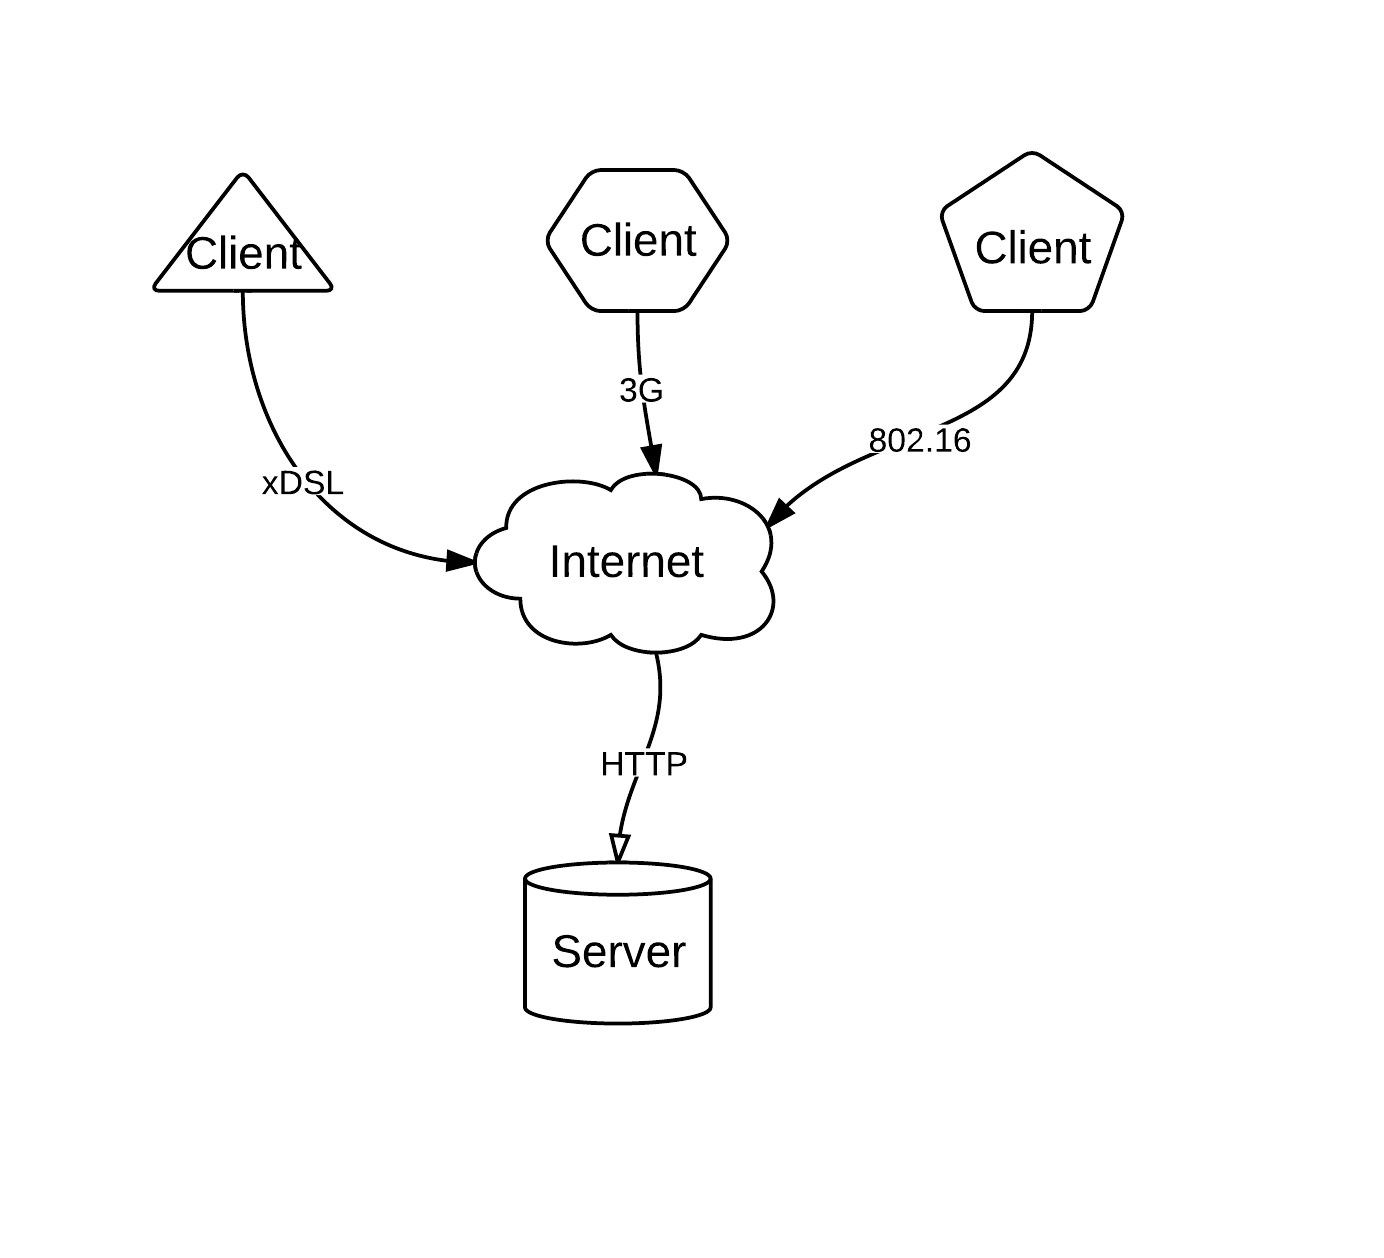
\includegraphics[scale=0.55]{images/cap2/Client-server.png}
\caption{Rappresentazione astratta architettura Client-Server}
\end{figure}
\end{center}

Il nucleo di Woty, dove viene gestita tutta la logica e vengono mantenuti i dati, risiede su un server centrale. Il server ospita il DBMS contentente i dati persistiti e l'applicazione web che tramite tali dati permette l'interazione con il sistema.\\
Woty è progettata per essere indipendente dal tipo di client che si interfaccerà con il server. Questo è garantito da un approccio orientato alla risorsa e da delle reference API standard. In questo modo la futura estensibilità di Woty verso nuovi tipi di client è non solo possibile, ma soprattutto semplice e realizzabile tramite un minimo costo implementativo.\\


\subsection{Woty: orientato alla risorsa}
Ogni ''elemento'' interno di woty (e.g. una quest, un utente, un achievement, etc) è offerto all'esterno come \emph{risorsa}. Questo permette la realizzazione di un approccio standard al webservice e garantisce massima estendibilità. \\
Ogni risorsa è disponibile all'esterno secondo precise regole di business (autorizzazioni, gestione della visibilità, etc.) in modo da aver sì un approccio standard, ma allo stesso tempo di avere un elevato grado di sicurezza, di incapsulamento delle informazioni e una personalizzazione ad-hoc per ogni risorsa senza limiti prestabiliti.


\subsection{Approccio RESTful}

Representational State Transfer, di seguito REST, è uno stile architetturale che permette la modellazione dei \emph{business models} tramite \emph{resources} (risorse). Le risorse sono rese accessibili tramite protocollo HTTP sotto forma di web services, e disponibili in varie \emph{representations}. Ogni risorsa espone metodi CRUD (\emph{create}, \emph{read}, \emph{update}, \emph{delete}) che vengono mappati su get, put, post, delete del protocollo HTTP. Il software che adotta questo tipo di struttura è definito come ''orientato alla risorsa''.\\

La tipologia di rappresentazione della risorsa richiesta è identificata sull'estensione del file identificato all'interno dell'uri. Ad esempio, una delle rappresentazioni disponibili è quella che incapsula le informazioni in sorgenti interpretabili da un web browser.\\ 

Un'altra caratteristica di questo approccio è la mancanza di necessità di tenere traccia dello stato. Ogni metodo è sempre disponibile o nascosto, senza dipendenze dallo stato del processo in esecuzione.\\ 
Tramite questa architettura si ottengono:

\begin{itemize}
			
\item Possibilità di comporre semplici richieste relazionali direttamente da uri.

\item API pubblica e autenticata, senza necessità di duplicazione di codice

\item Interfaccia di comunicazione tra i gli strati presentation e logic

\item Stretto legame con le risorse effettivamente presenti su database

\item State-less design (anche le sessioni sono modellate su risorse)

\item Sicurezza concentrata su singolo componente (HTTPS)
			
\item Disaccoppiamento tra i due strati comunicanti
\end{itemize}

Questo tipo di approccio aumenta l'estensibilità e la scalabilità del software. Rende inoltre il codice uniformato per risorse, facilmente comprensibile quindi meno dipendente dalle competenze del programmatore. \\
L'effettiva implementazione del webservice mappa tramite uri non solamente i metodi CRUD ma anche le operazioni (azioni index, show, edit) utili alla effettiva esecuzione dei metodi.\\
I seguenti metodi sono esplicitati maggiormente nel paragrafo \ref{resource}.
		
\begin{longtable}{|p{3cm}|p{5,0cm}|p{3cm}|}
\caption{HTTP/URI/CRUD}\\
\hline
\endfirsthead
\multicolumn{3}{r}{\textit{(Continua alla pagina successiva)}}
\endfoot
\multicolumn{3}{l}{\textit{(Continua dalla pagina precedente)}}
\endhead
\hline
\endlastfoot
\textbf{HTTP Verb} & \textbf{URI}& \textbf{Action}\\
\hline
POST & /resource & CREATE (C)\\
\hline
GET & /resource/id & SHOW (R)\\
\hline
PUT & /resource/id & UPDATE (U)\\
\hline
DELETE & /resource/id & DELETE (D)\\
\hline
GET & /resource & INDEX\\
\hline
GET & /resource/new & NEW\\
\hline
GET & /resource/id/edit & EDIT\\
\hline
\end{longtable}

\section{Woty - Standard di sviluppo}

\subsection{Webservice}
\subsubsection{Applicazione Web}
La scelta del team Sevenfold, per la realizzazione dell'applicazione web, è ricaduta su Ruby on Rails (RoR).\\
Ruby on Rails, di seguito RoR, è un framework opensource relativamente giovane sviluppato sul linguaggio interpretato Ruby. La caratteristica principale che lo differenzia rispetto alla concorrenza consta nella community di contributors che direttamente o indirettamente rendono disponibili librerie facilmente installabili tramite RubyGems. Il framework rende estremamente astratta la modellazione della realtà sollevando il programmatore dalla progettazione di buona parte della struttura architetturale di un software basato sul web. 
\\Per il suo utilizzo cosciente quindi è necessaria la conoscenza del dietro le quinte, che a sua volta ha bisogno di competenze acquisite in precedenza riguardo paradigmi, design pattern e best practice di programmazione.
\subsubsection{DBMS}
IL DBMS utilizzato è MySql. Le caratteristiche del framework RoR, tuttavia, permettono di portare l'applicazione su svariati altri DBMS con il minimo sforzo, essendo RoR \emph{DBMS-agnostic} e le modifiche alla struttura del DB basate su migrazioni (oggetti logici, senza nessun tipo di sintassi SQL che potrebbe essere non supportata in tutti i DBMS).

\subsection{Client Desktop}
Il client desktop (un piccolo tool di che permette la notifica di quest assegnatae all'utente e l'accesso rapido alla web application di Woty) è stato realizzato in C++ mediante il framework Qt.\\
Questa scelta è dovuta al fatto che si è voluto garantire la massima compatibilità con i diversi sistemi operativi (il client funziona correttamente su Windows, Linux e OsX). Lo stesso risultato si sarebbe potuto ottenere con Java, ma l'overhead prestazionale della JVM è stato valutato negativo, soprattutto considerando che il client si carica all'avvio dell'OS e resta resident nella toolbar fino alla chiusura. 

\subsection{Client Android}
Nel nostro ambito Java viene utilizzato per la creazione di un'applicazione interfacciabile su dispositivi mobile con sistema operativo Android. La versione utilizzata è Android SDK 2.2, al fine di permettere alla quasi totalità dei dispositivi di ricevere notifiche push. Questo tipo di notifiche è reso possibile attraverso C2DM (Android Cloud to Device Messaging Framework). Le librerie grafiche utilizzate sono quelle fornite da Android, mentre per l'interfacciamento al Cloud è stato fatto riuso di codice messo a disposizione direttamente dal team di Google. 


\section{Architettura soluzione}

In figura \ref{StrutturaGeneraleSistema} viene riportata l'architettura generale della soluzione. Le componenti sono denominate: lato server, sistema di notifica, client web e client mobile. 

\begin{figure}[H]
\centering
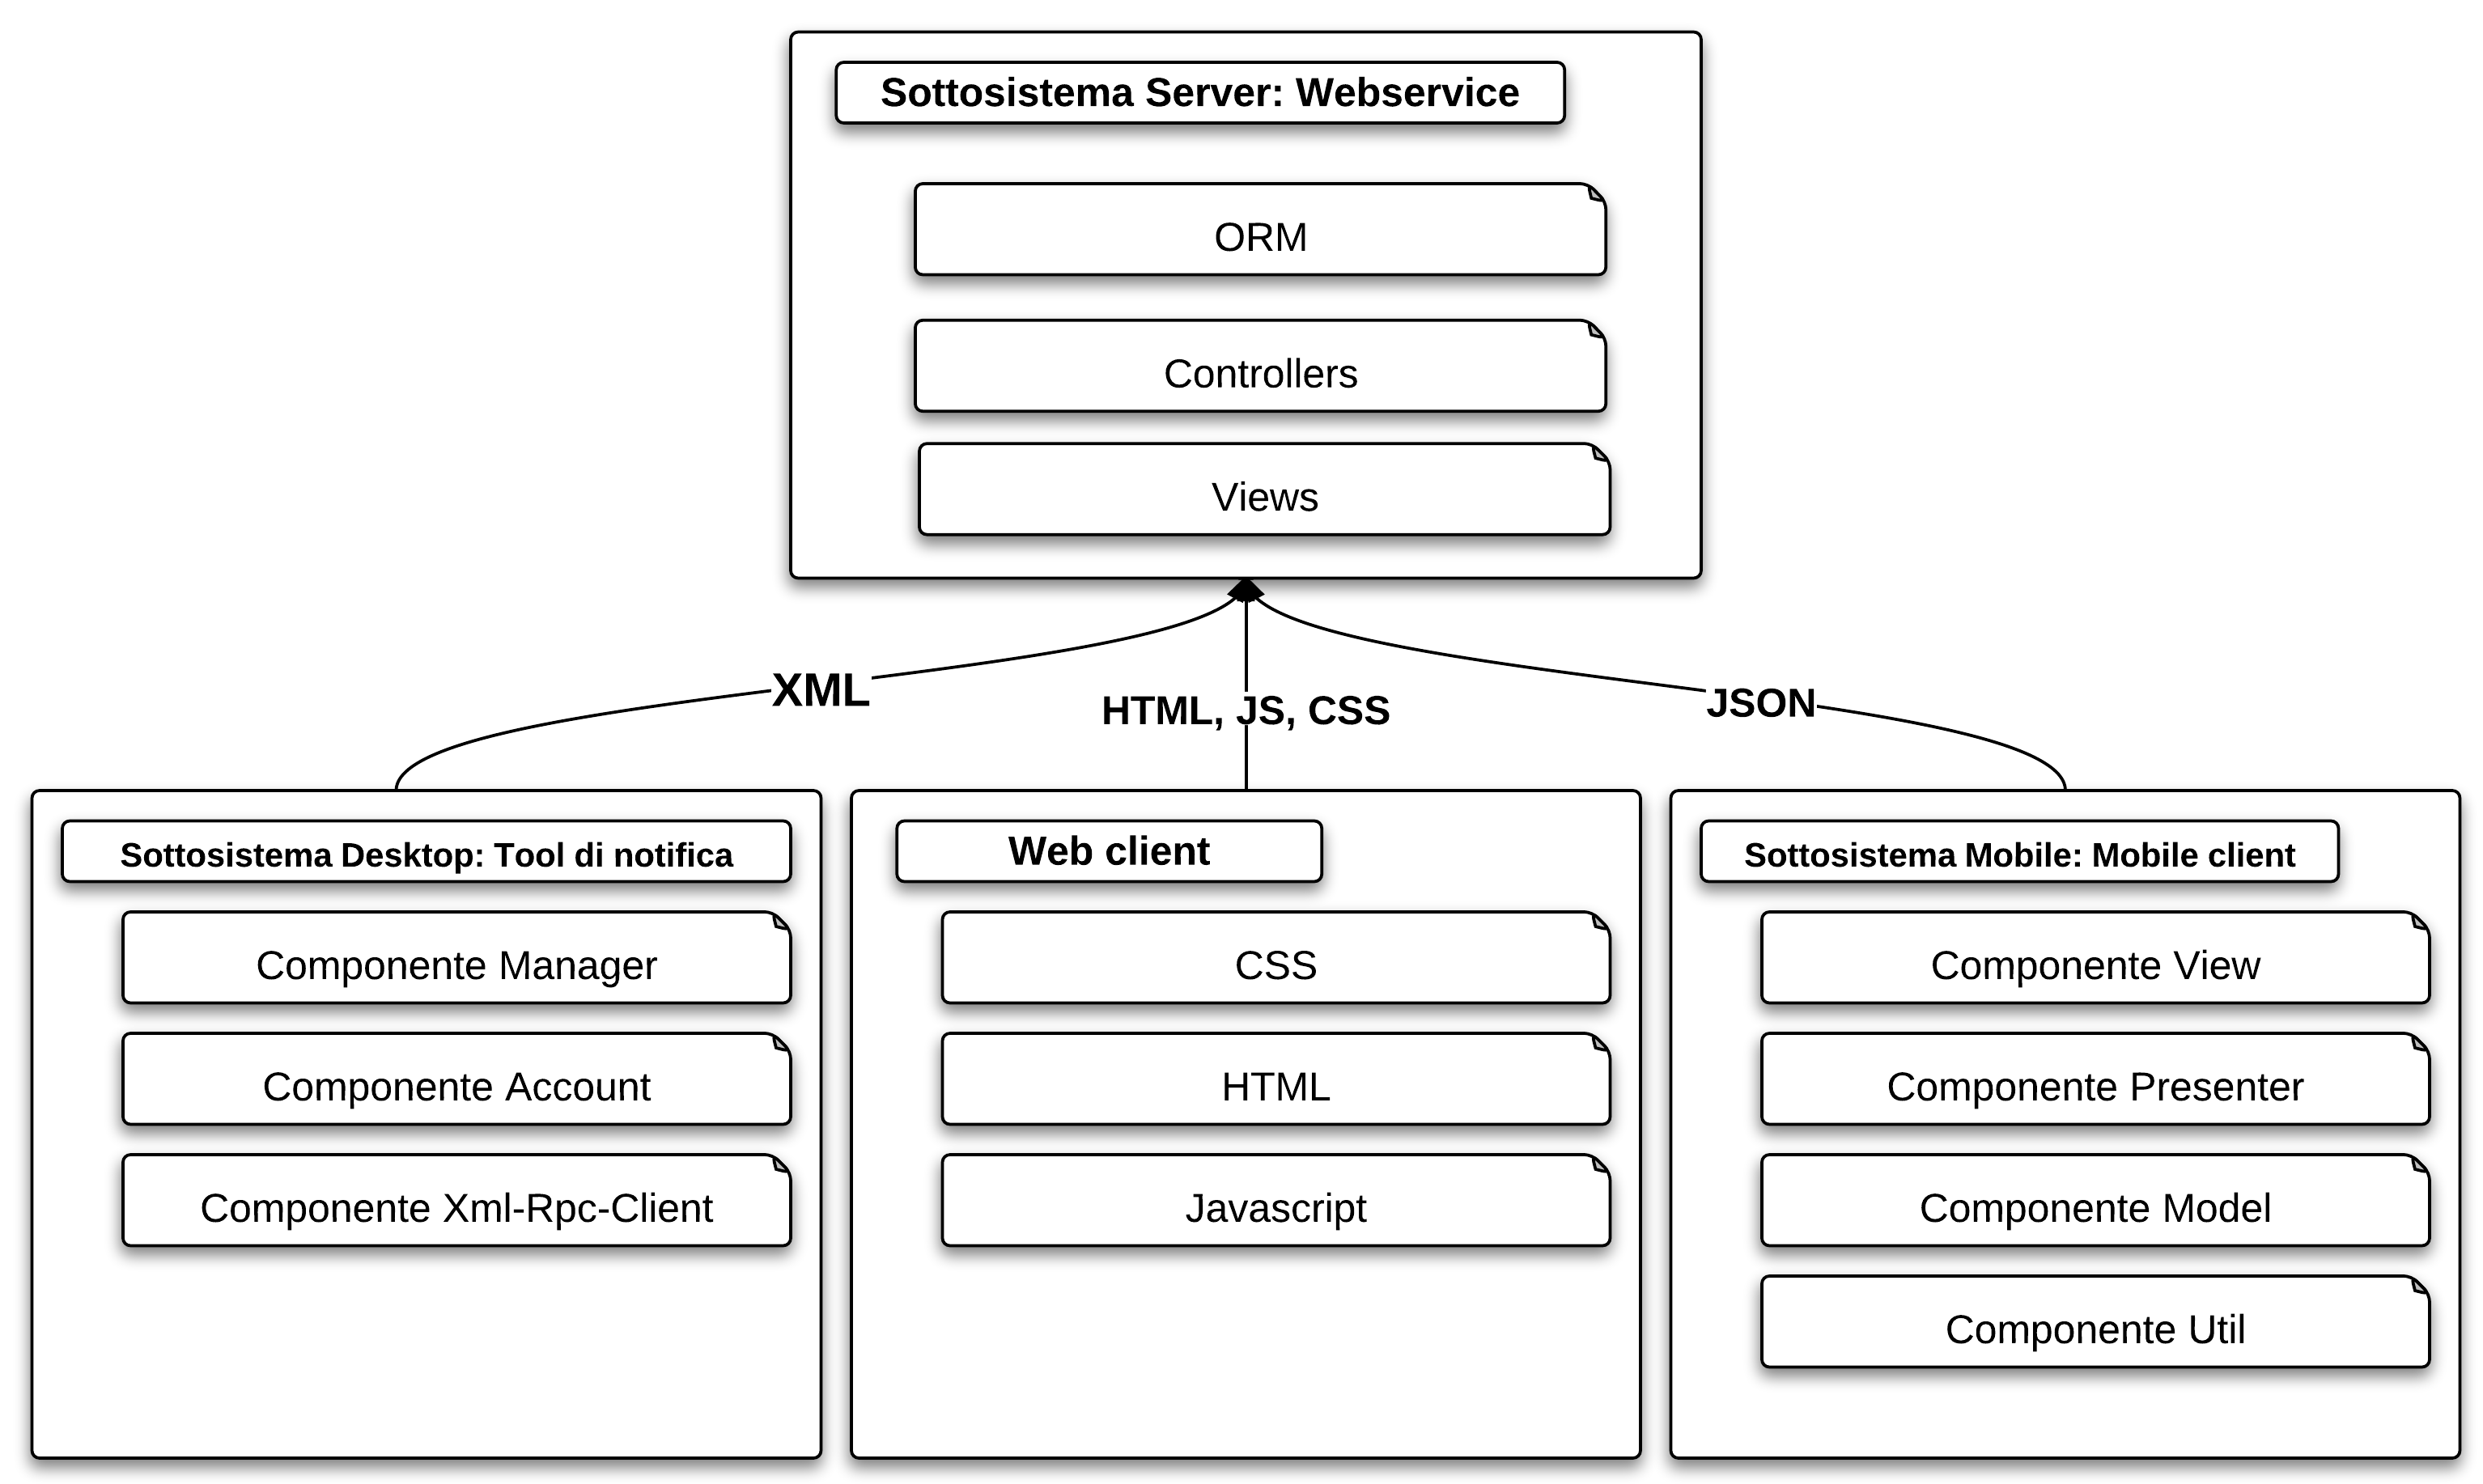
\includegraphics[scale=0.6]{images/cap2/sistema.png} % vedi Lateximpazienye pg67
\caption{Struttura generale del sistema}
\label{StrutturaGeneraleSistema}
\end{figure}



\subsection{Sottosistema Server: Webservice}
Il sottosistema server è responsabile della gestione di tutte le risorse di PMAC. Si occupa di interagire con i client, della conservazione e elaborazione dei dati. L'interazione con i web client è permessa attraverso la visualizzazione di pagine HTML, coadiuvate da fogli di stile CSS e di linguaggio lato client Javascript. L'interazione con i client mobile e i tool di notifica desktop è realizzata attraverso comunicazione di messaggi XML e JSON.

% inserire una figura
\begin{figure}[H]
\centering
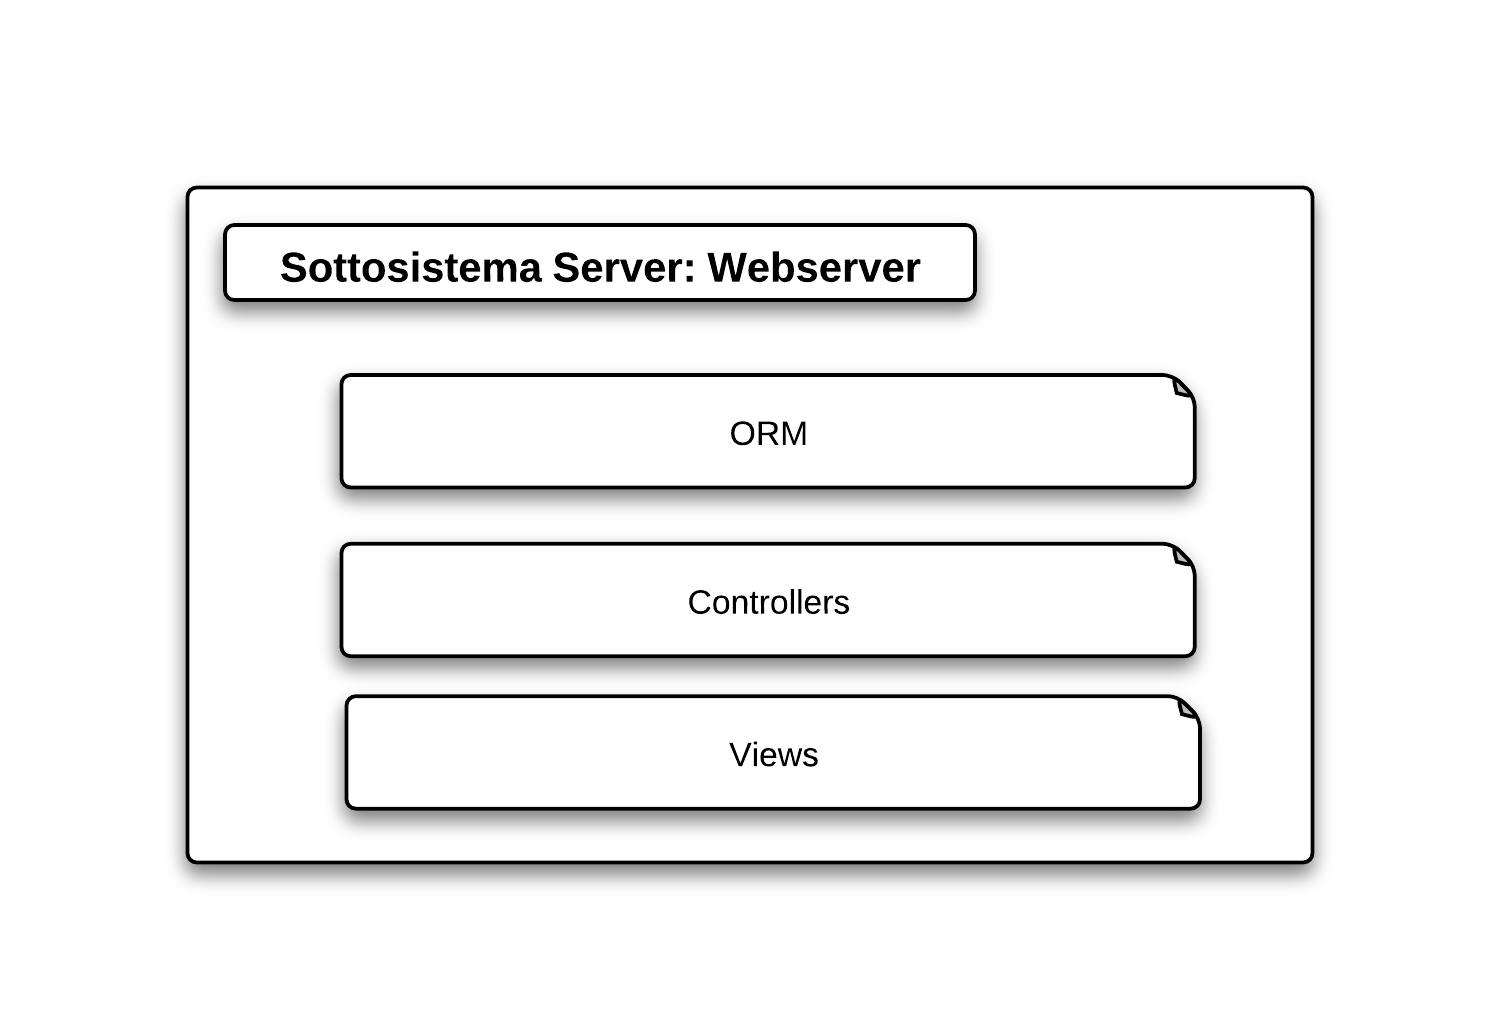
\includegraphics[scale=0.7]{images/cap2/Server/sottosistemaServer.png} % vedi Lateximpazienye pg67
\caption{Sottosistema Server}
\end{figure}

Nel presente documento è presente anche una descrizione più in dettaglio dell'architettura del sottosistema server, in modo da poter comprendere l'interfaccia che il webservice offre all'esterno, oltre che alle logiche interne.


\subsection{Sottosistema Desktop: Tool di notifica}

Il sottosistema Desktop si occupa di gestire la ricezione delle notifiche lato desktop per un utente del tipo Desktop-user, e consiste in una applicazione di tipo Tray Icon semplice ed intuitiva.\\
Una volta installata l'applicazione nell'apposito computer, il Desktop-user potrà effettuare il login al server PMAC attraverso le proprie credenziali. In questo modo l'applicazione potrà controllare periodicamente la presenza di nuove quest da svolgere assegnate allo specifico utente, o in caso contrario, l'utente potrà richiederne di nuove.\\
Il sottosistema sarà implementato con l'utilizzo del linguaggio di programmazione object oriented C++, e il framework Qt correlato.\\
Tale sottosistema è stato suddiviso in tre componenti logici come illustrato nella figura \ref{Sottosistema Desktop}.


% inserire una figura
\begin{figure}[H]
\centering
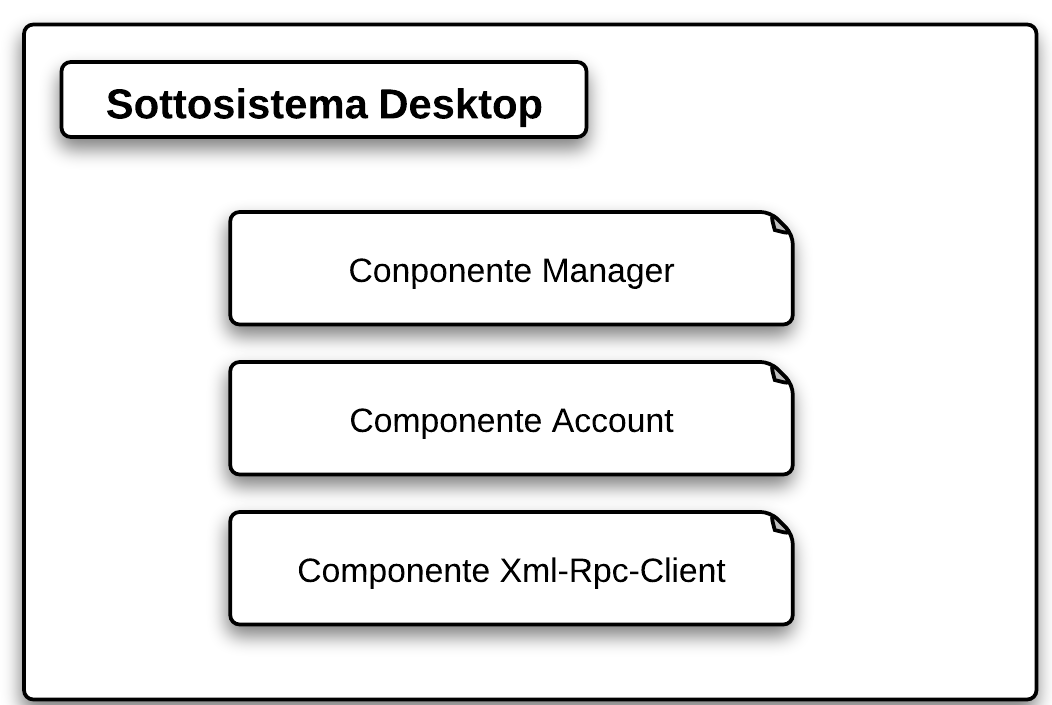
\includegraphics[scale=0.7]{images/cap2/Desktop/sottosistemaDesktop.png} % vedi Lateximpazienye pg67
\caption{Sottosistema Desktop}
\label{Sottosistema Desktop}
\end{figure}



\subsection{Sottosistema Mobile: Mobile client}
Il sottosistema mobile prevede lo sviluppo di un applicazione dedicata per il sistema operativo Android che offra all'utente un esperienza di navigazione alla pari, o più simile possibile, a quella offerta da una postazione fissa.\\
Questo sottosistema prevede l'interazione con il server per il recupero di tutte le informazioni necessarie e offre un servizio di notifiche push per la segnalazione della presenza di nuove Quest disponibili all'utente autenticato dal dispositivo mobile.\\
Per lo sviluppo architetturale abbiamo scelto di seguire il design pattern MVP, per una massima separazione ed estendibilità del codice.\\
Sono quindi stati previsti i seguenti componenti principali:
\begin{itemize}
\item Componente Model, che rappresenta i dati gestiti dall'applicazione.
\item Componente View, che consiste nelle classi che gestiscono l'interfaccia grafica proposta all'utente.
\item Componente Presenter che è incaricato di gestire le interazioni tra View e Model, in particolare riceve le notifiche generate dell'interazione dell'utente con l'interfaccia grafica e porta a termine le dovute funzioni tramite l'interazione con il Model.
\end{itemize}
Prevediamo poi l'utilizzo di package di supporto come util ed exceptions che forniscono funzionalità come quelle necessarie al parser e alla gestione delle eccezioni. Abbiamo ritenuto di separare questi componenti dal resto della struttura perché non appartengono al design pattern MVP.

% inserire una figura
\begin{figure}[H]
\centering
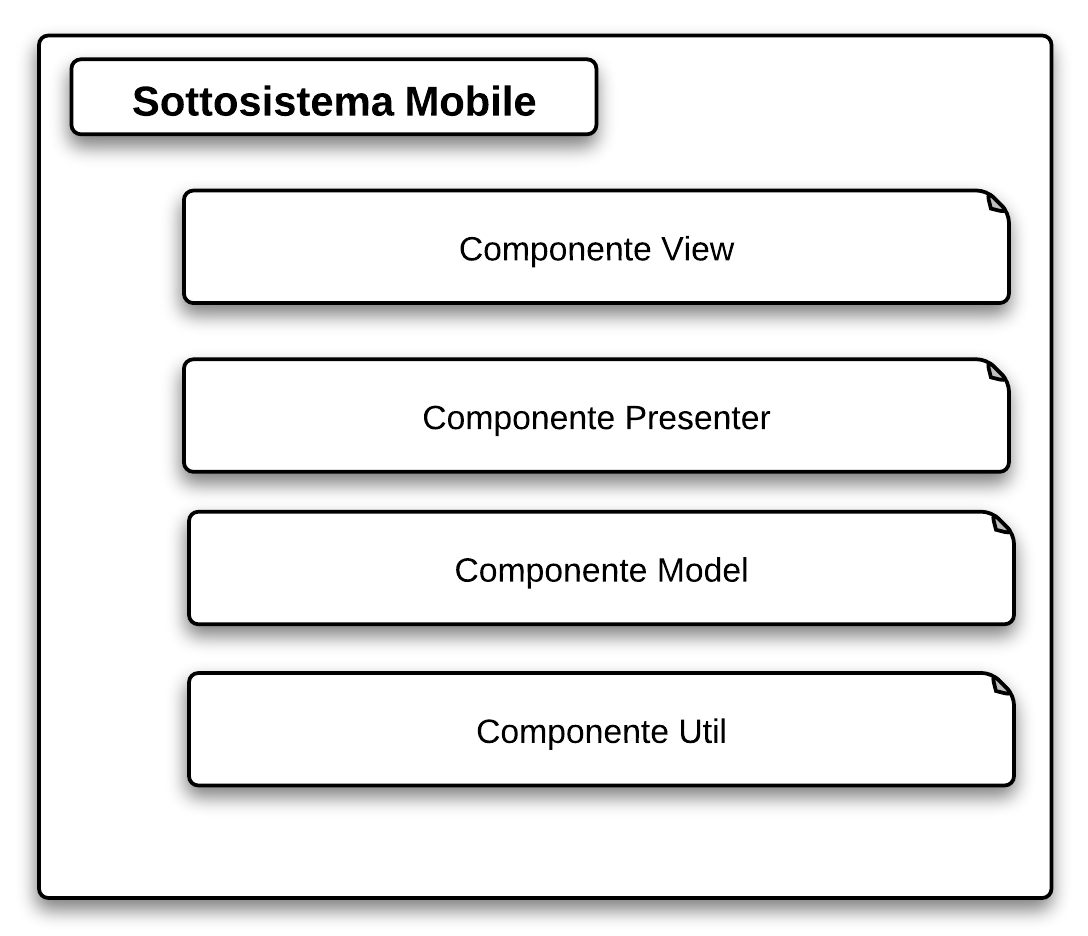
\includegraphics[scale=0.7]{images/cap2/Mobile/sottosistemaMobile.png} % vedi Lateximpazienye pg67
\caption{Sottosistema Mobile}
\end{figure}


\subsection{Web client}
Il web client è un'interfaccia modulare per l'accesso e la modifica dei contenuti utente. Abbiamo identificato due tipologie di pagine web:

\begin{itemize}
\item Pagine di accesso alle risorse, derivate dalle necessità CRUD
\item Pagine statiche, derivate da altri requisiti (es. informazioni del software)
\end{itemize}

Le prime saranno uniformate rispetto ad ogni tipo di risorsa. Le seconde invece avranno layout e contenuti diversi. Riteniamo molto importante la fluidità e l'esperienza d'uso utente. Perciò ci avvaliamo di librerie esterne sicure per fogli di stile e javascript per il buon funzionamento cross-browser e il gusto visivo. Per le stesse ragioni in particolare Ajax ed elementi dinamici saranno utilizzati per simulare la responsività di una vera applicazione locale.

\section{Architettura sottosistema Server}

\subsection{Modalità di descrizione}
Nella presente sezione non verrà descritta ogni classe nel dettaglio, ma verrà utilizzato un approccio più ad alto livello, orientato alle funzionalità che il webservice offre verso l'esterno.
Le richieste esterne verranno effettuate attraverso l'interfaccia REST precedentemente specificata. Le richieste, quindi, saranno tutte verso risorse disponibili nel webservice. \\
Per questo motivo i diagrammi che seguono saranno orientati alla \emph{risorsa}, le varie classi rappresenteranno una classe logica per le risorse e per le risposte che il webservice può dare ad un generico client.

\subsection{Diagramma delle classi}

\subsubsection{HttpResponse}

\begin{figure}[H]
\centering
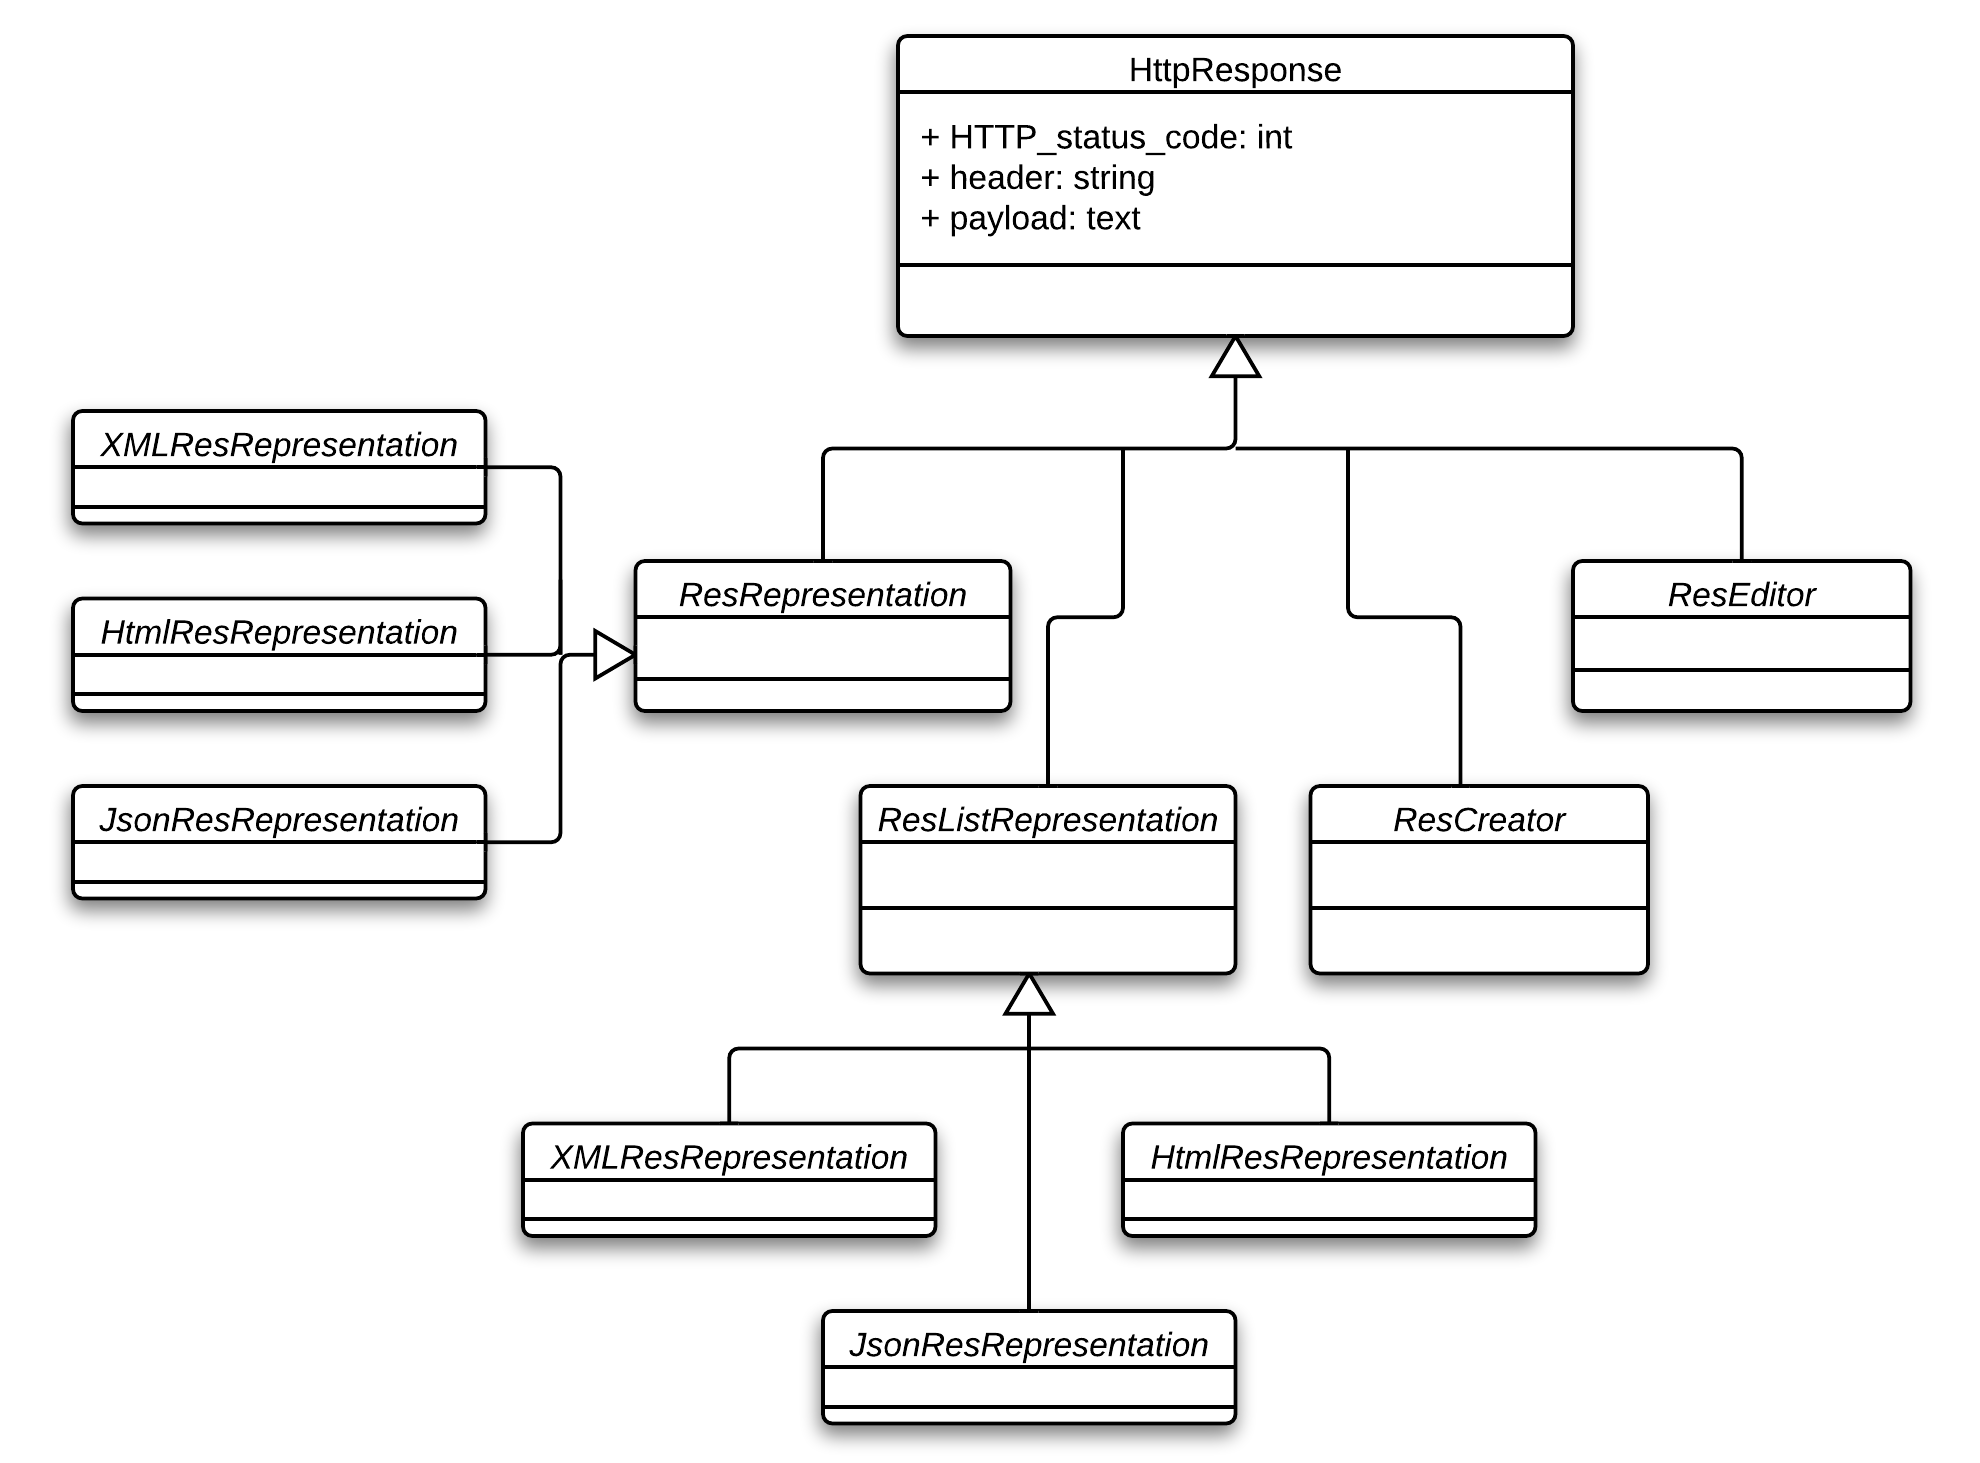
\includegraphics[scale=0.55]{images/cap2/Server/HttpResponse.png}
\caption{Server - HttpResponse}
\end{figure}

Lo scopo del diagramma è il presentare le risposte che il webservice può dare ad un generico client. Di seguito la descrizione delle classi:

\begin{itemize}
\item Classe HttpResponse: rappresenta la risposta HTTP che il webservice restituisce in seguito ad una richiesta REST. E' idealmente caratterizzata da 3 attributi:
\begin{itemize}
\item HTTP\_status\_code: è un intero che rappresenta l'esito della richiesta (e.g. 201 = Created, 401 = Unauthorized)
\item header: contiene meta-informazioni sul contenuto del payload
\item payload: è l'effettivo messaggio trasmesso tramite HTTP 
\end{itemize}
\item Classe ResEditor: è una HttpResponse contenente una vista HTML con la quale è possibile modificare i campi di una risorsa. Genericamente, una form.
\item Classe ResCreator: è una HttpResponse contenete una vista HTML con la quale è possibile creare una risorsa. Anche in questo caso, genericamente è una form.
\item Classe ResListRepresentation:  è una HttpResponse contente lista di istanze di una generica risorsa. Da essa ereditano le classe XMLResListRepresentation, HtmlResListRepresentation, JsonResListRepresentation le quali incapsulano la lista in, rispettivamente, XML, HTML, JSON.
\item Classe ResRepresentation: è una HttpResponse contenete una vista HTML che visualizza una risorsa.Da essa ereditano le classe XMLResRepresentation, HtmlResRepresentation, JsonResRepresentation le quali incapsulano la risorsa in, rispettivamente, XML, HTML, JSON.
\end{itemize}

\subsubsection{Resource}
\label{resource}

\begin{figure}[H]
\centering
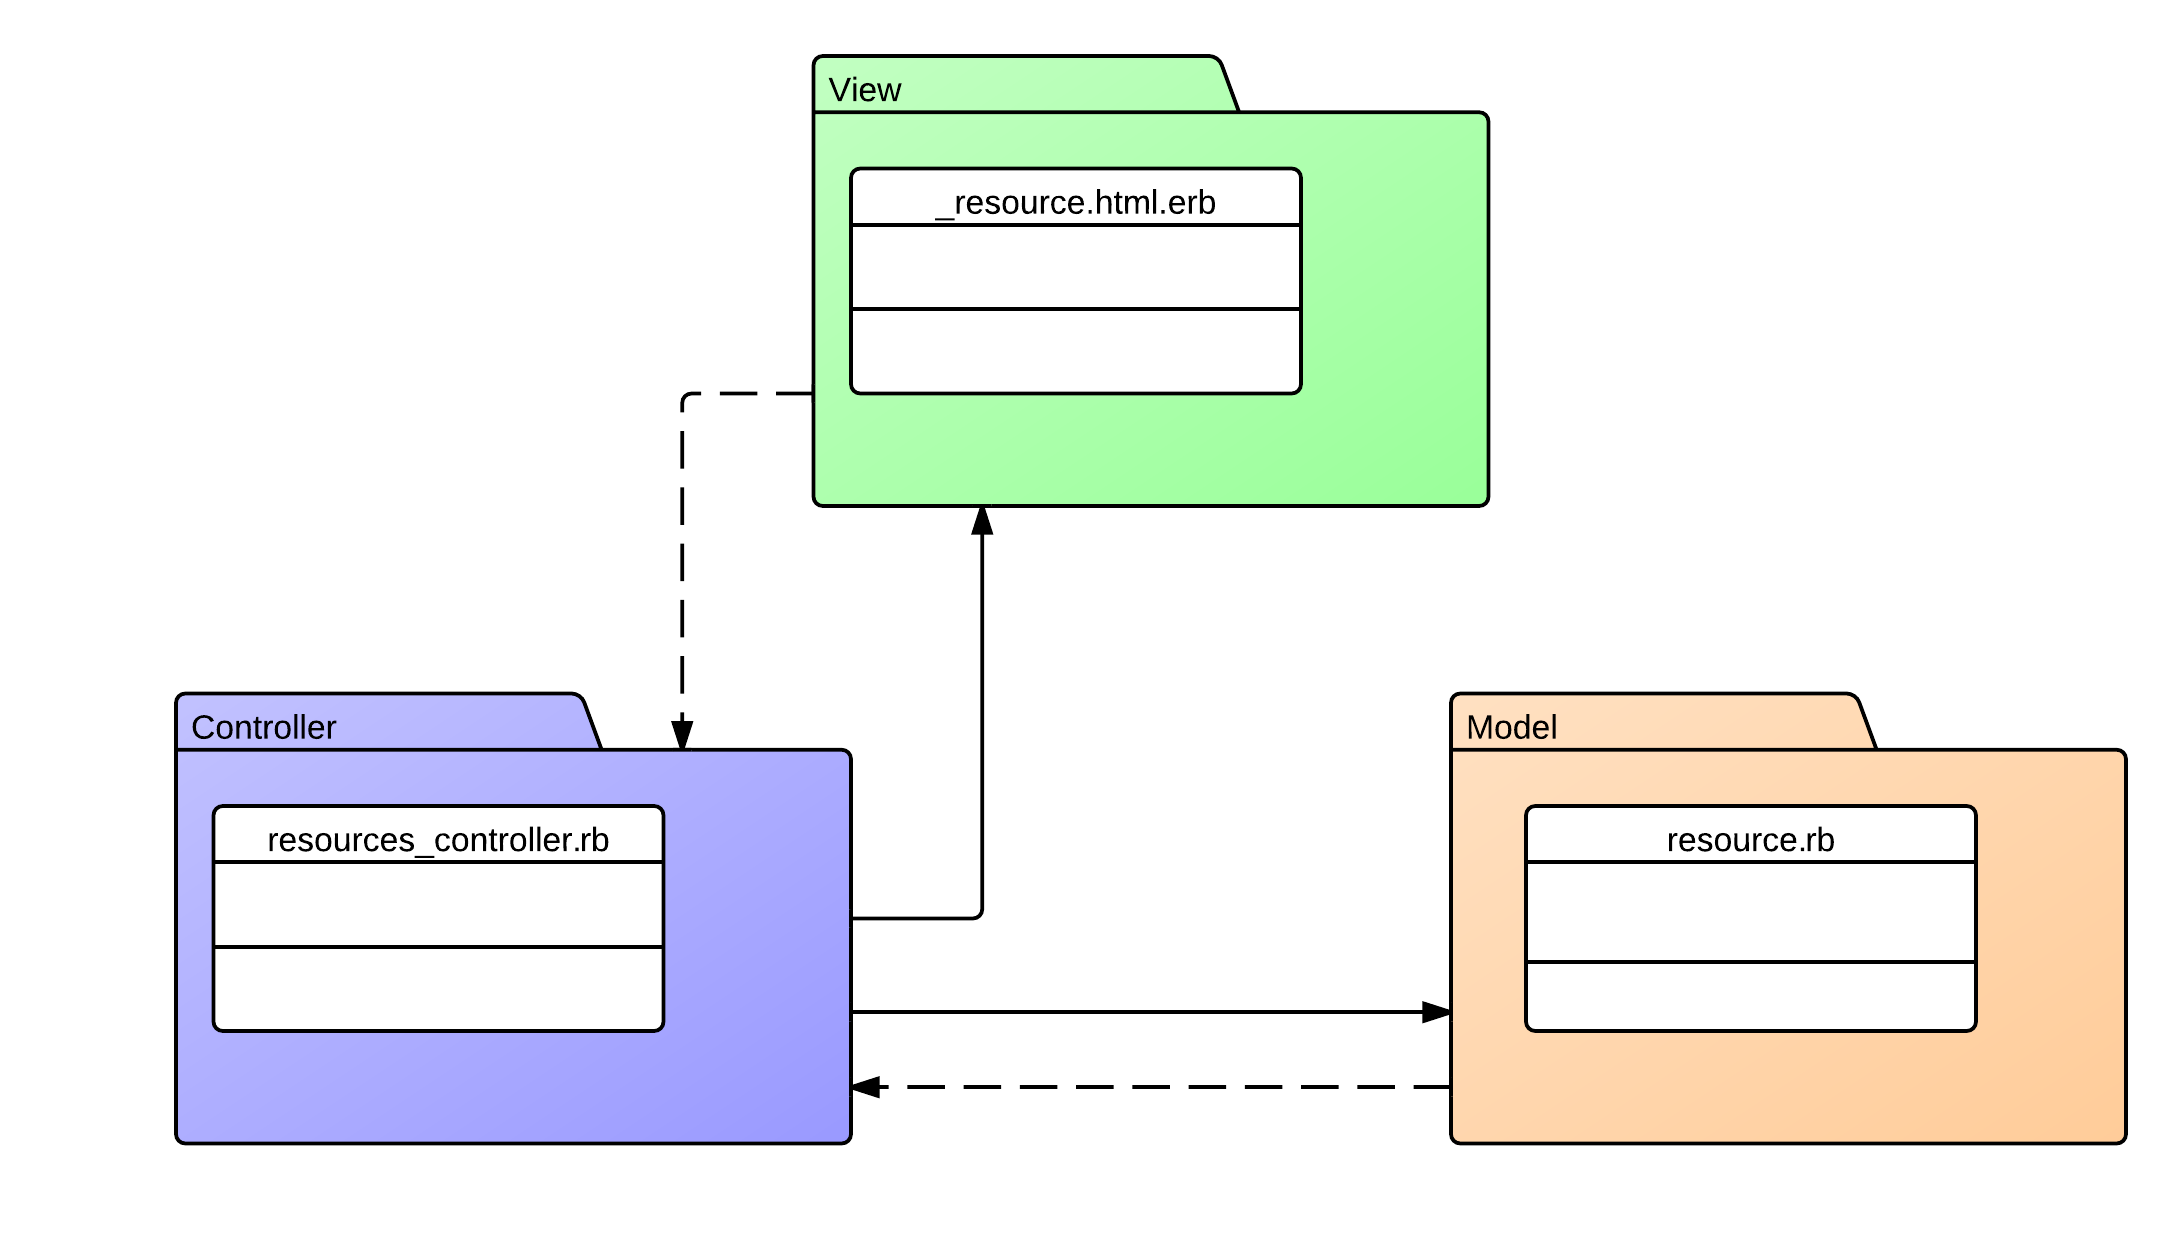
\includegraphics[scale=0.70]{images/cap2/Server/MvcResource.png}
\caption{Server - Resource generica}
\end{figure}

Nel diagramma è rappresentato come è mappata una resource generica secondo il modello model-view-controller del framework RoR.

\begin{figure}[H]
\centering
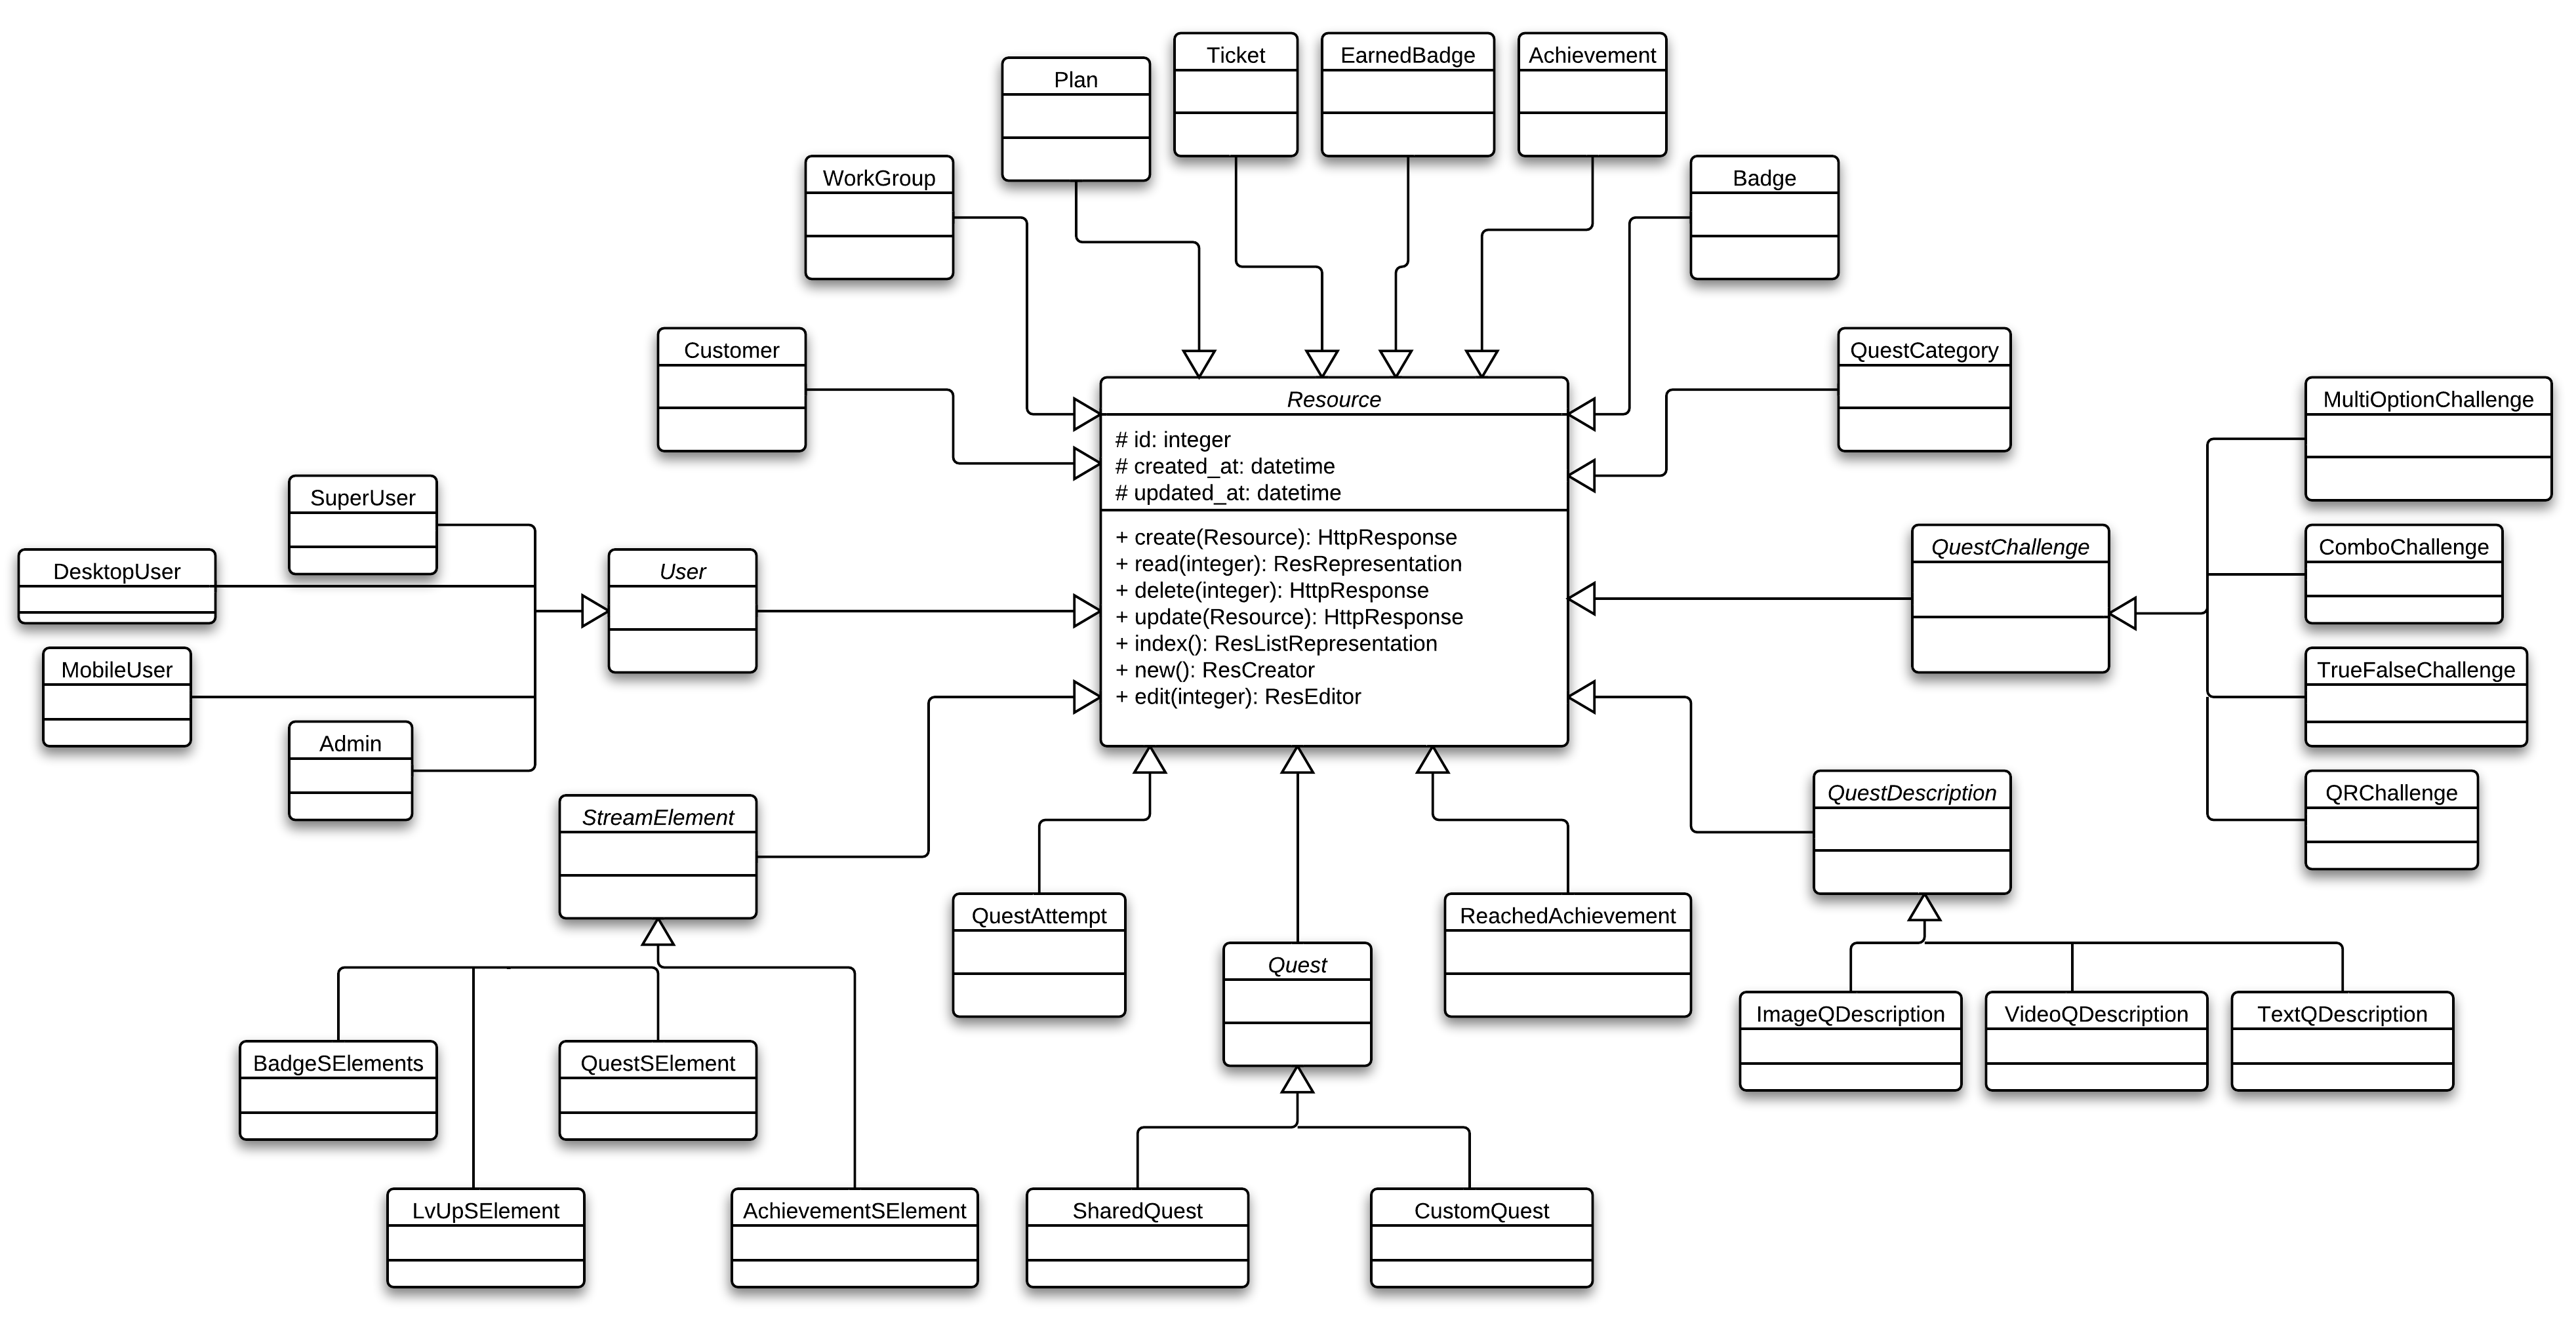
\includegraphics[scale=0.50]{images/cap2/Server/Resource.png}
\caption{Server - Resource}
\end{figure}

Questo diagramma vuole mostrare come ogni classe logica disponibile nel webservice sia in realtà una risorsa. Le relazioni e le dipendenze più dettagliate tra le classi saranno visibili in seguito nel diagramma degli oggetti in figura \ref{S-do}.\\


\subsubsection{Diagramma ad oggetti}
Il seguente diagramma ad oggetti vuole mettere in evidenza come una risorsa sia effettivamente una tabella nel DB, e le relazioni tra le varie risorse.

\begin{figure}[h]
\centering
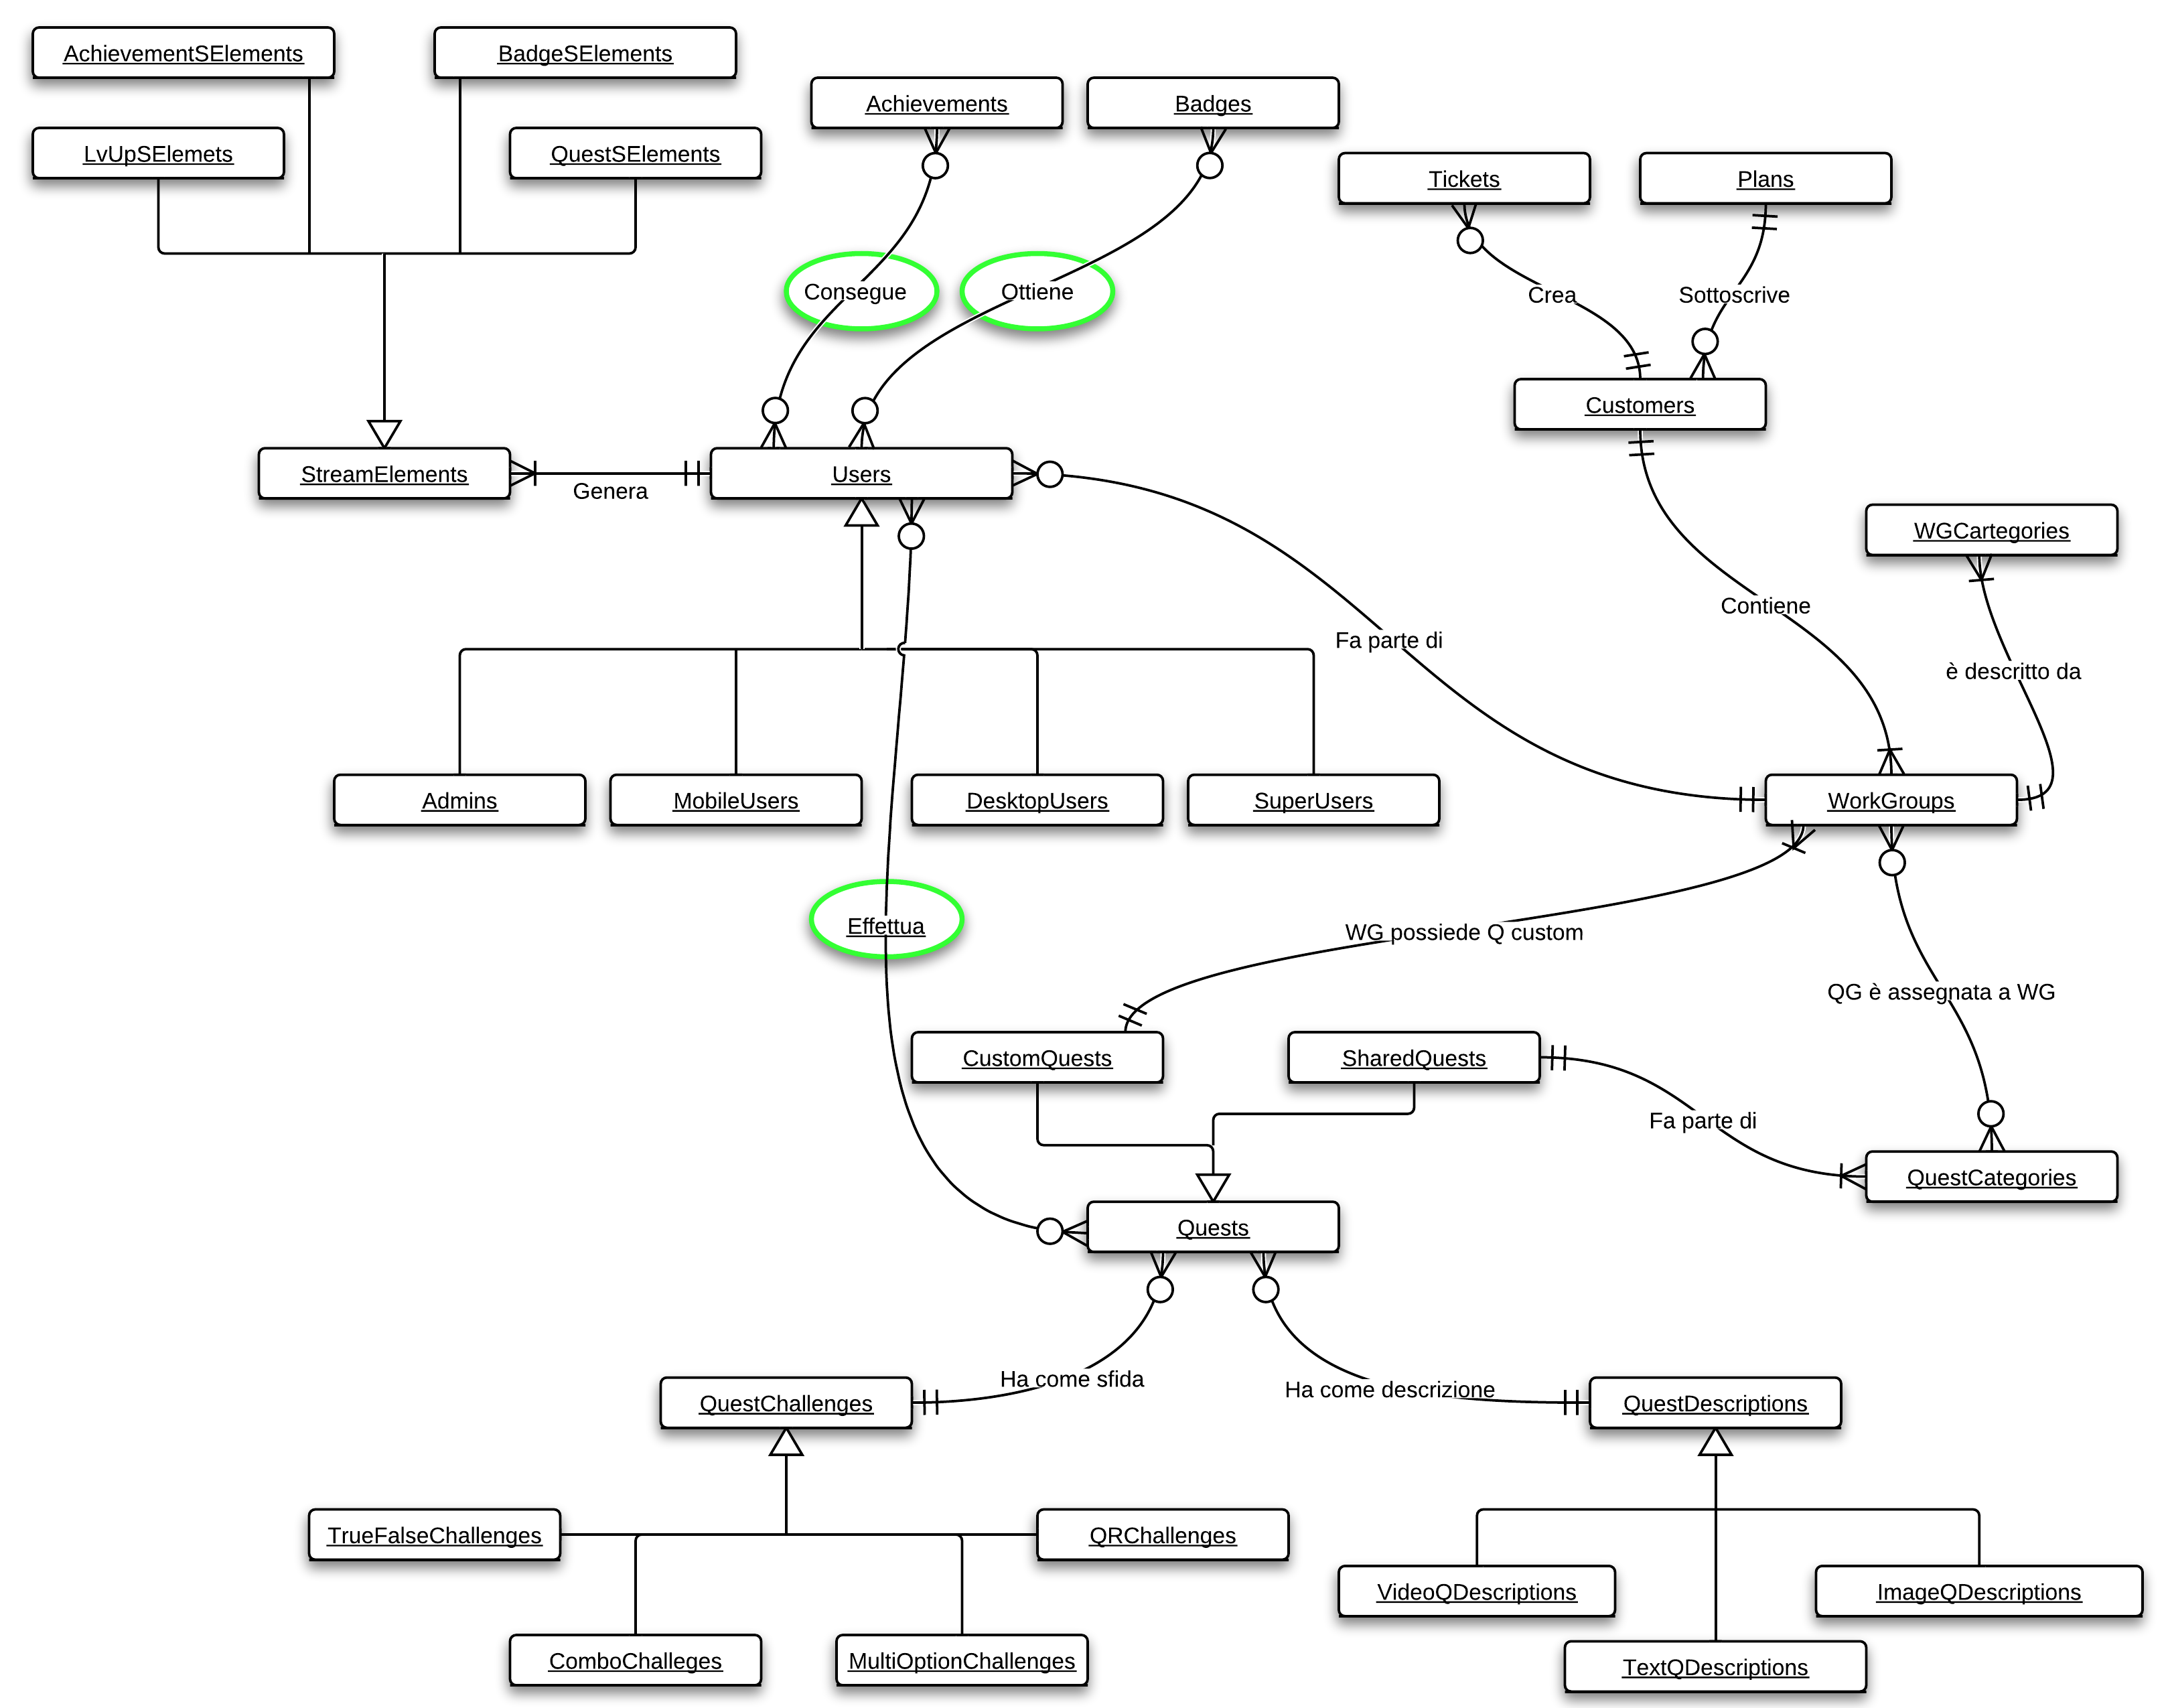
\includegraphics[scale=0.55]{images/cap2/Server/Oggetti.png}
\caption{Server - Diagramma ad oggetti}
\label{S-do}  % S-do = Server - diagramma oggetti
\end{figure}

Da notare il fatto che dalle relazioni N:M nascano delle risorse:

\begin{itemize}
	\item Dalla relazione Users <-> Quests nasce la risorsa QuestAttempt.
	\item Dalla relazione Users <-> Achievements nasce la risorsa ReachedAchievent.
	\item Dalla relazione Users <-> Badge nasce la risorsa EarnedBadge.
\end{itemize}

Altri punti che meritano una spiegazione:

\begin{itemize}
	\item Dalla relazione N:M WorkGroups <-> QuestCategories è stato deciso di non far emergere una risorsa, seppur una tabella debba necessariamente essere creata.
	\item L'entità WGCategories è una tabella nata per evitare ridondanze nella denominazione dei WorkGroup, non è stato quindi ritenuto necessario mapparla come risorsa.
\end{itemize}

\subsection{Descrizione risorse}
Verrà di seguito riportata una descrizione delle risorse di Woty, in modo da poter meglio comprendere cosa rappresentano e quali relazioni presentano tra di esse

\subsubsection{User} Utente base registrato al sistema. Classe base della gerarchia di utenti.
\subsubsection{SuperUser} Utente con priviliegi di SuperUser
\subsubsection{DesktopUser} Utente Desktop
\subsubsection{MobileUser} Utente Mobile
\subsubsection{Admin} Amministratore di Woty
\subsubsection{Customer} Risorsa che modella i clienti del fornitore del servizio. Ogni customer ha vari workgroup che a loro volta contengono una serie di user. Ogni customer inoltre sottoscrive un plan, che definisce il livello di servizio per il customer.\\
I costi quindi, sono calcolati tra questa classe e la classe Plan. Nel sistema è un'entità molto importante in quanto tutti gli utenti fruiscono dei contenuti all’interno del loro customer.\\
\subsubsection{WorkGroup} Classe che rappresenta un reparto di un’azienda cliente, che sono composti dagli utenti facenti parte dello stesso.\\
Gli utenti in reparti lavorano anche in team, e sono disponibili classifiche di reparto. Sono inoltre utilizzati per l’assegnazione delle quest, in quanto il reparto è una delle caratteristiche per le quali sono influenzate le categorie di rischio.
\subsubsection{Plan}Risorsa che modella le formule d’acquisto del prodotto. Il paradigma Software as a Service uniforma nel miglior modo possibile il maggior numero di clienti.\\
Per il nostro caso possono essere sottoscritti vari piani di acquisto e nel caso in cui il cliente necessiti di caratteristiche personali è possibile assegnare dei plan privati.\\
All’interno del plan sono definite alcune abilità che possono o meno essere utilizzate a seconda del prezzo pagato.
\subsubsection{Quest} La classe modella le quest e la loro composizione. Di fatto le quest sono composte di una descrizione e una sfida: entrambe possono essere di vario tipo e sono rappresentate tramite gerarchie.
Le quest inoltre hanno una categoria che può essere inclusa in un workgroup: gli utenti facenti parte sono in grado di svolgere le quest con le categorie associate.
\subsubsection{QuestDescription}Classe base della gerarchia inerente le tipologie di descrizione di una quest. La gerarchia è utilizzata per la composizione di una quest.
\subsubsection{TextDescription} Rappresenta una QuestDescription che contiene solo testo.
\subsubsection{ImageDescription} Rappresenta una QuestDescription che contiene un'immagine.
\subsubsection{VideoDescription} Rappresenta una QuestDescription che contiene un video.
\subsubsection{QuestChallenge} Classe base per le sfide delle quest. Rappresenta il componente sfida delle quest che può essere di varie tipologie, definite tramite le sottoclassi.
\subsubsection{ComboChallenge} Classe che rappresenta un quesito a risposta multipla con una ed una sola risposta corretta.
\subsubsection{TrueFalseChallenge} La classe modella una tipologia particolare di QuestChallenge contenente più affermazioni, ognuna delle quale può essere vera o falsa.
\subsubsection{MultiOptionChallenge} La classe modella una tipologia particolare di QuestChallenge contenente più affermazioni, ognuna delle quale può essere valida o meno. Si differenzia da TrueFalseChallenge a livello logico, in quanto più che possibili affermazioni che possono essere vere e false, modella possibili opzioni che possono essere valide o meno.
\subsubsection{Achievement} Gli achievement sono modellati tramite una serie di condizioni legate dall’operatore logico AND. Per semplicità di implementazione non si è ritenuta necessaria l’implementazione di altri operatori logici. La validità di un achievement è calcolata per uno user e valida tutte le condizioni associate.
\subsubsection{Like} Like è la risorsa che modella i like effettuati dagli utenti. Attualmente
è possibile effettuare i like solo su elementi membri della gerarchia StreamElement.
\subsubsection{StreamElemet}StreamElement è la classe base per gli elementi di attività visibili nel pannello utente. Le attività possono essere di vario genere, permettono l’interazione tramite like e commenti, e costituiscono il principale elemento social del sistema.
\subsubsection{QuestHistory} Una QuestHistory relaziona uno User con una Quest. Viene creata
quando uno User svolge una Quest oppure quando il sistema assegna ad uno User una Quest.
\subsubsection{Ticket}Rappresenta un Ticket creato da un SuperUser e rivolto al/agli Admin del sistema.
\subsubsection{CompletedAchievement}Rappresenta un achievement ottenuto da un utente.
\subsubsection{CompletedAchievementElement}Specializzazione della classe StreamElement che rappresenta l’ottenimento di un achievement da parte di un utente.
\subsubsection{Condition}La classe modella una condizione necessaria al completamento di un achievement. Le condizioni sono composte da un operatore, uno dei valori definiti in Achievable, e un valore fissato dal creatore. Abbiamo deciso di limitare la libertà di creazione delle condizioni, in quanto altre soluzioni sarebbero state troppo complesse da implementare. Il sistema le rende comunque generabili dinamicamente.
\subsubsection{CustomQuest}Modella una Quest personalizzata, disponibile solo ad un determinato Workgroup
\subsubsection{QuestCategory}Identifica una categoria di rischio al quale una SharedQuest è associata
\subsubsection{SharedQuest}Rappresenta una Quest condivisa tra più Workgroup





\end{document}
